\documentclass[12pt]{article}
\usepackage[colorlinks,citecolor=blue,urlcolor=blue]{hyperref}
\usepackage{amsmath}
\usepackage{amsfonts}
\usepackage{amssymb}
\usepackage{graphicx}
\usepackage{enumerate}
\usepackage{natbib}
\usepackage{url} % not crucial - just used below for the URL 
\usepackage{xcolor}
\usepackage{array}
\usepackage{bm}
\usepackage{multirow}
\usepackage{booktabs} 
\usepackage{adjustbox}
\usepackage{caption}
\usepackage{subcaption}
\usepackage{sectsty}
\usepackage{adjustbox}
\usepackage{longtable}
\usepackage[figuresright]{rotating}
\usepackage{multicol}
\usepackage{wrapfig}
\usepackage[plain,noend]{algorithm2e}
\usepackage{bbm}
\usepackage{newtxtext}
\usepackage{ulem}
\usepackage{amsthm}
\usepackage[subscriptcorrection]{newtxmath}
\usepackage[margin=1in]{geometry}

\newcommand{\blind}{0}
\graphicspath{{./figures/}}

% LaTeX macros

% Last modified: 24/2/2008


%----------------------------------------------
%  A. C. Davison, Institute of Mathematics,
%  EPFL, 1015 Lausanne, Switzerland
%  00 41 21 693 5502
%----------------------------------------------

% mathematical symbols, etc.
\usepackage{environ}
\usepackage{xcolor}

\definecolor{myorange}{HTML}{E24100}
\def\Rev#1{{\textcolor{myorange}{#1}}}
\def\Rem#1{{\iffalse #1 \fi}}
\def\Rep#1#2{{\textcolor{myorange} {#2}}}
\def\r{\color {red}}
\def\rr{\bf\color {red}}
\def\b{\color {blue}}

\NewEnviron{Res}{%
\noindent\textbf{Response: }\textcolor{myorange}{\BODY}
}

\NewEnviron{Comments}{%
\noindent\textsl{\BODY}
}

\newtheorem{lemma}{Lemma}
\newtheorem{theorem}{Theorem}
\newtheorem{proposition}{Proposition}
\newtheorem{corollary}{Corollary}
\newtheorem{definition}{Definition}

\def\dashfill{\cleaders\hbox{-}\hfill}
\def\dashline{\noindent\makebox[\linewidth]{\dashfill}}
\def\r{\color {red}}
\def\rr{\bf\color {red}}
\def\b{\color {blue}}

\def\half{{\textstyle{1\over 2}}}
\def\third{{\textstyle{1\over 3}}}
\def\quarter{{\textstyle{1\over 4}}}
\def\sixth{{\textstyle{1\over 6}}}
\def\frac#1#2{{\textstyle{#1\over#2}}}
\def\Beta{{\rm B}}

\def\argmin{{\rm argmin}}  
\def\diag{{\rm diag}}  
\def\mod{{\rm mod}}  
\def\tr{{\rm tr}}
\def\sign{{\rm sign}}
\def\ow{{\rm otherwise}}  
\def\obs{{\rm obs}}  
\def\endex{{\hfill{\color{red}$\bullet$}\medskip}}
\def\Endex{{\hfill{$\bullet$}\medskip}}
\def\redbf#1{{\color{red}\bf #1}}%
\def\red#1{{\color{red} #1}}%
\def\white#1{{\color{black} #1}}%

\DeclareSymbolFont{AMSb}{U}{msb}{m}{n}
\DeclareMathSymbol{\Natural}{\mathbin}{AMSb}{"4E}
\DeclareMathSymbol{\Integer}{\mathbin}{AMSb}{"5A}
\DeclareMathSymbol{\Real}{\mathbin}{AMSb}{"52}
\DeclareMathSymbol{\Rational}{\mathbin}{AMSb}{"51}
\DeclareMathSymbol{\Imaginary}{\mathbin}{AMSb}{"49}
\DeclareMathSymbol{\Complex}{\mathbin}{AMSb}{"43} 
\DeclareMathSymbol{\Disk}{\mathbin}{AMSb}{"44} 
\def\bi{\begin{itemize}}
\def\ei{\end{itemize}}
\def\bd{\begin{description}}
\def\ed{\end{description}}
\def\ben{\begin{enumerate}}
\def\een{\end{enumerate}}
\def\bv{\begin{verbatim}}
\def\ev{\end{verbatim}}

\def\bth{{$b{\rm th}$ }}
\def\cth{{$c{\rm th}$ }}
\def\dth{{$d{\rm th}$ }}
\def\fth{{$f{\rm th}$ }}
\def\gth{{$g{\rm th}$ }}
\def\hth{{$h{\rm th}$ }}
\def\ith{{$i{\rm th}$ }}
\def\jth{{$j{\rm th}$ }}
\def\kth{{$k{\rm th}$ }}
\def\lth{{$l{\rm th}$ }}
\def\mth{{$m{\rm th}$ }}
\def\nth{{$n{\rm th}$ }}
\def\pth{{$p{\rm th}$ }}
\def\rth{{$r{\rm th}$ }}
\def\sth{{$s{\rm th}$ }}
\def\tth{{$t{\rm th}$ }}
\def\uth{{$u{\rm th}$ }}
\def\vth{{$v{\rm th}$ }}
\def\wth{{$w{\rm th}$ }}

\def\calA{{\mathcal A}}
\def\calB{{\mathcal B}}
\def\calC{{\mathcal C}}
\def\calD{{\mathcal D}}
\def\calE{{\mathcal E}}
\def\F{{\mathcal F}}
\def\G{{\mathcal G}}
\def\H{{\mathcal H}}
\def\calH{{\mathcal H}}
\def\IG{{\mathcal IG}}
\def\cI{{\mathcal I}}
\def\cP{{\mathcal P}}
\def\calJ{{\mathcal J}}
\def\calL{{\mathcal L}}
\def\calK{{\mathcal K}}
\def\calM{{\mathcal M}}
\def\calN{{\mathcal N}}
\def\N{{\calN}}
\def\calP{{\mathcal{P}}}
\def\calQ{{\mathcal{Q}}}
\def\calO{{\mathcal{O}}}
\def\calS{{\mathcal{S}}}
\def\calI{{\mathcal{I}}}
\def\calR{{\mathcal R}}
\def\calT{{\mathcal T}}
\def\calU{{\mathcal U}}
\def\calV{{\mathcal V}}
\def\calW{{\mathcal W}}
\def\calX{{\mathcal X}}
\def\calY{{\mathcal Y}}
\def\calZ{{\mathcal Z}}
\def\W{{\mathcal W}}
\def\U{{\Upsilon}}
\def\f{\frac}
\def\l{{\lambda}}
\def\d{{\delta}}
\def\bX{{\bar X}}
\def\s{{\sigma}}
\def\p{{\partial}}
\def\p{{d}}
\def\v{{\varepsilon}}
\def\dis{{\displaystyle}}
\def\a{{\alpha}}
\def\b{{\beta}}
\def\hash{{\#}}
\def\bar#1{{\overline{#1}}}
\def\hat#1{{\widehat{#1}}}
\def\barY{{\overline{Y}}}
\def\barX{{\overline{X}}}
\def\barZ{{\overline{Z}}}
\def\barx{{\overline{x}}}
\def\bary{{\overline{y}}}
\def\barz{{\overline{z}}}
\def\T{{ \mathrm{\scriptscriptstyle T} }}
\def\mT{{ -\mathrm{\scriptscriptstyle T} }}
\newcommand{\indep}{\perp\!\!\!\perp}
\newcommand{\nindep}{\perp\!\!\!\perp\!\!\!\!\!\!/\;\;}

\newcommand{\med}{{\rm med}}
\newcommand{\card}{{\rm card}}
\newcommand{\bs}{\boldsymbol}
% \newcommand{\do}{{\rm do}}
\newcommand{\Splus}{\textsc{S-Plus}\ }
%\newcommand{\R}{\texttt{R} }

% Bold notation
\def\bR{{\boldsymbol{R}}}
\def\bS{{\boldsymbol{S}}}
\def\bZ{{\boldsymbol{Z}}}
\def\bQ{{\boldsymbol{Q}}}
\def\bN{{\boldsymbol{N}}}
\def\bP{{\boldsymbol{P}}}
\def\bX{{\boldsymbol{X}}}
\def\ba{{\boldsymbol{a}}}
\def\bb{{\boldsymbol{b}}}
\def\bx{{\boldsymbol{x}}}
\def\by{{\boldsymbol{y}}}
\def\bw{{\boldsymbol{w}}}
\def\bs{{\boldsymbol{s}}}
\def\bt{{\boldsymbol{t}}}
\def\bv{{\boldsymbol{v}}}
\def\bu{{\boldsymbol{u}}}
\def\bz{{\boldsymbol{z}}}

\def\real{{\mathbb R}}
%\def\reald{{\mathbb R}^d}

% statistical notation

\def\rmi{{\rm i}}
\def\pr{{\rm Pr}}
\def\Pr{\pr}
\def\E{{\rm E}}
\def\Ev{{\rm Ev}}
\def\var{{\rm var}}
\def\avar{{\rm avar}}
\def\cov{{\rm cov}}  
\def\corr{{\rm corr}}  
\def\Estar{{\rm E^*\thinspace}}
\def\varstar{{\rm var^*\thinspace}}
\def\covstar{{\rm cov^*\thinspace}}  
\def\median{{\rm median}}  
\def\cum{{\rm cum}}
\def\IMSE{{\rm IMSE}}  
\def\AIC{{\rm AIC}}  
\def\BIC{{\rm BIC}}  
\def\NIC{{\rm NIC}}  
\def\AICc{{\rm AIC_c}}  
\def\CV{{\rm CV}}  
\def\GCV{{\rm GCV}}  
\def\IQR{{\rm IQR}}  
\def\MAD{{\rm MAD}}  
\def\Lik{{L}}
\def\logL{{\ell}}
\def\RLik{{RL}}
\def\logLp{{\ell_{\rm p}}}
\def\eqd{{\stackrel{\mathrm{d}}{=}}}
\def\Dto{{\ {\buildrel D\over \longrightarrow}\ }}
\def\dto{{\ {\buildrel d\over \longrightarrow}\ }}
\def\Pto{{\ {\buildrel P\over \longrightarrow}\ }}
\def\rto{{\ {\buildrel r\over \longrightarrow}\ }}
\def\2to{{\ {\buildrel 2\over \longrightarrow}\ }}
\def\Wto{{\ {\buildrel W\over \longrightarrow}\ }}
\def\psto{{\ {\buildrel \rm{p.s.}\over \longrightarrow}\ }}
\def\asto{{\ {\buildrel \rm{a.s.}\over \longrightarrow}\ }}
\def\iid{{\ {\buildrel \rm{iid}\over \sim}\ }}
\def\ind{{\ {\buildrel \rm{ind}\over \sim}\ }}
\def\dotsim{{\ {\buildrel \cdot\over \sim}\ }}
%\def\sim{{\ {\sim}\ }}
%\def\to{{\longrightarrow}}
\def\Deq{{\ {\buildrel D\over =}\ }}
\def\Eoneton{{$E_1,\ldots,E_n$}}
%\def\T1ton{{$T_1,\ldots,T_n$}}
\def\I1ton{{$I_1,\ldots,I_n$}}
%\def\U1ton{{$U_1,\ldots,U_n$}}
\def\X1ton{{$X_1,\ldots,X_n$}}
\def\Y1ton{{$Y_1,\ldots,Y_n$}}
\def\Z1ton{{$Z_1,\ldots,Z_n$}}
\def\R1ton{{$R_1,\ldots,R_n$}}
\def\e1ton{{$e_1,\ldots,e_n$}}
\def\t1ton{{$t_1,\ldots,t_n$}}
\def\x1ton{{$x_1,\ldots,x_n$}}
\def\y1ton{{$y_1,\ldots,y_n$}}
\def\z1ton{{$z_1,\ldots,z_n$}}
%\def\r1ton{{$r_1,\ldots,r_n$}}

% Journal abbreviations

\def\AAP{\emph{Advances in Applied Probability}}
\def\AnnProbab{\emph{Annals of Probability}}
\def\AISM{\emph{Annals of the Institute of Statistical Mathematics}}
\def\AMS{\emph{Annals of Mathematical Statistics}}
\def\ApplStatist{\emph{Applied Statistics}}
\def\AS{\emph{Annals of Statistics}}
\def\B{\emph{Bernoulli}}
\def\Bka{\emph{Biometrika}}
\def\CJS{\emph{Canadian Journal of Statistics}}
\def\CSDA{\emph{Computational Statistics \& Data Analysis}}
\def\Eca{\emph{Econometrica}}
\def\ISI{\emph{International Statistical Review}}
\def\ISR{\emph{International Statistical Review}}
\def\JAMA{\emph{Journal of the American Medical Association}}
\def\JAP{\emph{Journal of Applied Probability}}
\def\JASA{\emph{Journal of the American Statistical Association}}
\def\JBES{\emph{Journal of Business \& Economic Statistics}}
\def\JCGS{\emph{Journal of Computational and Graphical Statistics}}
\def\JSCS{\emph{Journal of Statistical Computation and Simulation}}
\def\JRSSA{\emph{Journal of the Royal Statistical Society series A}}
\def\JRSSB{\emph{Journal of the Royal Statistical Society series B}}
\def\JRSSD{\emph{The Statistician}}
\def\SJS{\emph{Scandinavian Journal of Statistics}}
\def\SPA{\emph{Stochastic Processes and their Applications}}
\def\SM{\emph{Survey Methodology}}
\def\SS{\emph{Statistical Science}}
\def\TAS{\emph{The American Statistician}}
\def\Tech{\emph{Technometrics}}
\def\ZW{\emph{Z. Wahrsch. v. geb.}}
\def\JC{\emph{Journal of Classification}}
\def\PNAS{\emph{Proceedings of the National Academy of Science}}

% utility macros

\def\np{{\newpage}}
\def\gap{{\vskip 0.3in}}
\def\etal{{\sl et al.}} 
\def\pound{{\it \$}}
\def\apriori{{\sl a priori }}
\def\examfoot{{\vfill\hfill{\bf Turn over}\eject}}
\def\newtransparency{{\newpage}}
\def\Section{{Section~}}
\def\Sections{{Sections~}}
\def\Pvalue{{P-value}}
\def\Pvalues{{P-values}}

\def\report#1{{\newpage\centerline{\bf #1}\smallskip}}

% odds and ends

\def\redbf#1{{\color{red}\bf #1}}%
\def\Defn{\redbf{Definition:\ }}%
\def\Thm#1{\redbf{Theorem #1:\ }}%
\def\Ex#1{\redbf{Example #1:\ }}%
\def\Note{\redbf{Note:\ }}%
\def\Exercise#1{\redbf{Exercise #1:\ }}%
\def\Ill{\redbf{Illustration:\ }}%
\def\endex{{\hfill\redbf{$\bullet$}\smallskip}}
\def\calP{{\mathcal{P}}}
\def\calS{{\mathcal{S}}}
\def\calI{{\mathcal{I}}}
\def\eme{{\`eme}}
\def\ere{{\`ere}}
%\def\picbox#1#2{{\centerline{\psfig{figure=#1,height=#2pc}}}}%
\def\picbox#1#2#3{{\centerline{\psfig{figure=#1,height=#2pc,angle=#3}}}}%
\def\tt#1{{\texttt{#1}}}
\def\Der#1{\textbf{D#1}}


\newcommand{\PZ}{\textcolor{orange}}

% Per-author symbol footnotes (no number superscripts)
% \symfoot{counter}{text} : places symbol marker + footnote text
\newcommand{\symfoot}[2]{%
  \begingroup
  \renewcommand{\thefootnote}{\fnsymbol{footnote}}%
  \setcounter{footnote}{#1}%
  \footnote{#2}%
  \endgroup
}
% \symfootmark{counter} : places symbol marker only, no footnote text
\newcommand{\symfootmark}[1]{%
  \begingroup
  \renewcommand{\thefootnote}{\fnsymbol{footnote}}%
  \setcounter{footnote}{#1}%
  \footnotemark%
  \endgroup
}

\begin{document}

%%%%%%%%%%%%%%%%%%%%%%%%%%%%%%%%%%%%%%%%%%%%%%%%%%%%%%%%%%%%%%%%%%%%%%%%%%%%%%
%\title{\bf Fast and efficient inference for flexible spatial extremes models}
% \title{ \bf Fast and flexible inference for spatial extremes}
\title{\bf \PZ{Fast spectral inference for max-stable and $r$-Pareto processes with a continuous exponent function}}
\if0\blind{
  \author{Peng Zhong\symfoot{1}{\PZ{School of Mathematics and Physics, University of Wollongong, Australia. Email: pzhong@uow.edu.au}}
  \and Scott A.~Sisson\symfootmark{2}
  \and Boris B\'{e}ranger\symfoot{2}{School of Mathematics and Statistics, UNSW Sydney, Australia. Email: \{scott.sisson, b.beranger\}@unsw.edu.au}}
  \maketitle
} \fi

\vspace{-8mm}
\baselineskip=25pt
\begin{abstract}
    Statistical modelling of spatial extreme events has gained increasing attention over the last few decades with max-stable processes, and more recently $r$-Pareto processes, becoming the reference tools for the statistical analysis of asymptotically dependent data. Although inference for $r$-Pareto processes is easier than for max-stable processes, there remain major hurdles for their application to high dimensional datasets within a reasonable timeframe. In addition, both approaches have almost exclusively focused on the Brown-Resnick model, for its Gaussian foundations, and for the continuity of its exponent measure. In this paper, we derive a class of models for which this continuity property holds and present the \emph{skewed Brown-Resnick} model, an extension of the Brown-Resnick that allows for non-stationarity in the dependence structure, and the \emph{\PZ{multivariate} truncated extremal-$t$} model, \PZ{defined for a finite number of locations}.
    % a refinement of the well-known extremal-$t$ model. 
    We use an inference methodology based on the intensity function of the process which is derived from the exponent measure, and demonstrate the statistical and computational efficiency of this approach. Applications to two real-world problems illustrate valuable gains in modelling flexibility as well as appealing computational gains over reference methodologies. 
\end{abstract}

\noindent{\it Keywords:}  Spatial extremes, $r$-Pareto process, max-stable process, spectral likelihood.
% \vfill

\baselineskip=25pt

%%%%%%%%%%%%%%%%%%%%%%%%%%%%%%%%%%%%%%%
%%%%%%%%%%%%%%%%%%%%%%%%%%%%%%%%%%%%%%%
%%%%%%%%%%%%%%%%%%%%%%%%%%%%%%%%%%%%%%%
\section{Introduction}
%%%%%%%%%%%%%%%%%%%%%%%%%%%%%%%%%%%%%%%
%%%%%%%%%%%%%%%%%%%%%%%%%%%%%%%%%%%%%%%
%%%%%%%%%%%%%%%%%%%%%%%%%%%%%%%%%%%%%%%

Statistical modelling of spatial extremes is of major importance for the management and assessment of risks inherent to spatial processes. Modelling the dependence structure in spatial extremes is an active field of research where parametric approaches for asymptotic models face major inferential hurdles and are mostly based on the Brown-Resnick model \citep{Brown.Resnick:1977, Kabluchko.etal:2009}, inhibiting realistic applications in high dimensions, $D$. For example, environmental processes are often observed over large spatial regions and/or with fine resolution, and having $D$ in the order of thousands is not uncommon. In this paper, we demonstrate that these inferential issues can be greatly reduced by using the intensity function as long as the exponent measure is continuous. We establish conditions for this property to hold and leverage it to construct new flexible models. 

When extreme events are defined as the maxima recorded over a long period of time, max-stable processes \citep{deHaan:1984, Schlather:2002} provide a wide class of models for asymptotically dependent data. However, the likelihood function of such models is intractable in high dimensions unless low-dimensional approximations are used, such as the composite likelihood \citep{Padoan.etal:2010,Davison.etal:2012, Whitaker.etal:2020} and the Vecchia approximation \citep{Huser.Zhong:2023}, which are suitable for dimension up to 1000. A relatively recent alternative spatial modelling framework defines extreme events as the realisations of a process for which a risk functional exceeds some high threshold. The corresponding limiting $r$-Pareto processes \citep{Ferreira.deHaan:2014, Dombry.Ribatet:2015, deFondeville.Davison:2018, deFondeville.Davison:2022} share the same theoretical foundations as max-stable processes. The likelihood for $r$-Pareto processes is more tractable than for max-stable processes but still requires evaluation of an intractable normalising constant, which can be avoided through e.g.~score matching \citep{deFondeville.Davison:2018,Lederer.Oesting:2023} or choosing the $L_1$-norm as the risk functional. However, methods based on low-dimensional approximations do not provide reasonable estimates for data with complex dependence structures (nonstationarity, anisotropy) due to their loss of higher-order dependence information, and score matching for $r$-Pareto processes is computationally unstable and might not converge when dependence is weak. 
Spectral likelihoods are an alternative likelihood-based method that use the likelihood function of a limiting multivariate Poisson point process of the max-stable process \citep{Coles.Tawn:1991,Engelke.etal:2015,Wadsworth.Tawn:2014}. The same likelihood can also be adopted for the corresponding $r$-Pareto process by choosing the $L_1$-norm as the risk functional. The spectral likelihood is computationally efficient and provides consistent estimates for high-dimensional data with complex dependence structures. However, its computational efficiency needs the assumption that the exponent measure is continuous, which is not always the case for existing models. Likelihood-free alternatives using neural networks \citep{Lenzi.etal:2023} and neural Bayes estimators \citep{Sainsbury.Zammit.Huser:2024, Richards.etal:2024} scale well with large $D$, but they involve a computationally heavy training phase, require fine model tuning, and do not provide any statistical guarantees. Almost all $r$-Pareto process models
%of the above references 
focus on the counterpart of the max-stable Brown-Resnick process, which we call the Brown-Resnick $r$-Pareto process, 
%for simplicity, 
due to its simple intensity function and its greater flexibility over other models \citep[see, e.g.,][]{deFondeville.Davison:2018, Richards.etal:2024, Hector.Reich:2024}.          


% \citet{Wadsworth.Tawn:2014} proposed a censoring approach that is more robust but computationally demanding (examples with $D=16$ but can reach $D\approx 30$), motivating the scoring rules based approach of \citet{deFondeville.Davison:2018} that is applicable to scenarios where $D$ is a few thousands. Nevertheless, this gradient scoring approach still requires significant computing power ($\approx$1-6 hours using 16 cores for $D=3,600$ spatial locations) and might not converge when the dependence is too weak. 

Both max-stable and $r$-Pareto processes exhibit asymptotic dependence, meaning they have persisting tail dependence as events become more extreme. \PZ{One can argue that many environmental applications display asymptotic independence \citep[e.g.,][]{Bopp.etal:2021, Huser.Wadsworth:2019} or weakening dependence, however, the empirical evidence is only demonstrated by showing the empirical estimates of joint tail exceedance probability with an increasing threshold, which results in great uncertainty in the empirical estimates. Therefore, it is not always clear whether the process is indeed asymptotically independent or if the spatial dependence has simply weakened to some low but relatively positive level. This justifies the needs of more flexible asymptotically dependent models, which remains the backbone of the spatial extreme value analysis and opens doors for further extension into other areas, such as graphical models.}

The overarching aim of this paper is to define a framework for modelling spatial extremes that allows for a broad class of dependence structures, as well as fast and efficient inference. The contributions of this manuscript are multi-fold: we (a) establish theoretical conditions for max-stable and $r$-Pareto models to have a continuous exponent measure; (b) derive new max-stable and $r$-Pareto models which offer greater flexibility than Brown-Resnick models in describing anisotropic dependence structures; %where composite 
%likelihood 
%and Vecchia likelihoods
%\citet{Huser.Zhong:2023} 
%fail to capture the local anisotropic dependence structure; 
(c) provide a fast inference methodology using spectral likelihoods that relies on continuity of the exponent measure and is applicable to both \PZ{max-stable and $r$-Pareto models}; and (d) improve the efficiency of state-of-the-art simulation algorithms for $r$-Pareto processes.    

The remainder of this paper is organised as follows: Section~\ref{sec:modelling} provides some background on 
%how to 
modelling the dependence structure between spatial extremes using max-stable and $r$-Pareto processes, while Section~\ref{sec:inference} summarises different strategies to fit parametric models. After these foundations,
%are established, 
we provide our theoretical contributions in Section~\ref{sec:theory}, which includes the construction of the skewed Brown-Resnick and truncated extremal-$t$ models. Experiments are conducted on synthetic data in Section~\ref{sec:sim} to showcase the efficiency of the proposed inference methodology. Finally, two real data analyses involving fitting both max-stable and $r$ -Pareto models are presented in Section~\ref{sec:real} to illustrate the computational superiority of the proposed methodology over state-of-the-art approaches, and to highlight the gains in flexibility of the dependence structure from the skewed Brown-Resnick model over the Brown-Resnick model.  

% high dimensional for logistic and nested (Vettori)
% mostly BR
% not definiing existing events, Davison et al 2012 provide some advice, time to move away from max-stable processes

%%%%%%%%%%%%%%%%%%%%%%%%%%%%%%%%%%%%%%%
%%%%%%%%%%%%%%%%%%%%%%%%%%%%%%%%%%%%%%%
%%%%%%%%%%%%%%%%%%%%%%%%%%%%%%%%%%%%%%%
\section{Modelling approaches for spatial extremes}
\label{sec:modelling}
%%%%%%%%%%%%%%%%%%%%%%%%%%%%%%%%%%%%%%%
%%%%%%%%%%%%%%%%%%%%%%%%%%%%%%%%%%%%%%%
%%%%%%%%%%%%%%%%%%%%%%%%%%%%%%%%%%%%%%%

% Let $X_i(\bs), i=1,2,\ldots$, be independent and identically distributed copies of a real-valued stochastic process $\{X(\bs),\bs\in\calS\}$ with continuous sample paths on the space $\calS \subset \real^2$, and for any finite set of spatial locations $\{\bs_1,\dots,\bs_D\}\subseteq\calS$, let $\bX=(X(\bs_1),\dots,X(\bs_D))^\top$ be the corresponding finite-dimensional random vector.
% % , and $\bm X=(X(s_1),\dots,X(s_D))^\top$ be a $D$-dimensional random vector at , with joint distribution $F$. 
% Note that throughout bold fonts are used to represent vectors unless otherwise stated. 

%%%%%%%%%%%%%%%%%%%%%%%%%%%%%%%%%%%%%%%
%%%%%%%%%%%%%%%%%%%%%%%%%%%%%%%%%%%%%%%
% \subsection{Max-stable processes}
%%%%%%%%%%%%%%%%%%%%%%%%%%%%%%%%%%%%%%%
%%%%%%%%%%%%%%%%%%%%%%%%%%%%%%%%%%%%%%%

% If there exist continuous functions $a_n(\bs)>0$ and $b_n(\bs)\in\real$ such that the limiting process
% %
% \begin{align}
% \label{eq:msp}
% Z(\bs) = \lim_{n \rightarrow \infty} \max_{i=1, \ldots, n} \frac{X_i(\bs) - b_n(\bs)}{a_n(\bs)},
% \end{align}
% has non-degenerate marginals, then $Z(\bs)$ is a max-stable process \citep[][Ch.~9]{deHaan.Ferreira:2006}. The finite-dimensional distribution of $Z(\bs)$, denoted by $G$, is max-stable and therefore its marginals follow the generalized extreme value distribution. 
A max-stable process, $Z$,  with unit Fr\'{e}chet margins can be characterized as
\begin{equation}
\label{eq:spectralrepresentation}
	Z(\bs) = \sup_{i=1}^\infty R_iW_i(\bs),\ \bs\in\calS, 
%    \ R_i \sim \text{PPP}(1/r),\ \text{for}\  r > 0,
\end{equation}
%
where $R_1, R_2, \ldots$, are the points of a Poisson Point Process (PPP) on $(0, \infty)$ 
%with mean measure $\upkappa(\cdot)$ 
and $W_1(\bs), W_2(\bs), \ldots$, are independent copies of a stochastic processes $W(\bs)$ on $\calS$ with unit mean \citep{deHaan.Ferreira:2006, Schlather:2002}.
%
The exponent measure restricted onto $\mathbb R^D_+$, denoted by $\upkappa$, is given by
%
\begin{equation}
\label{eq:exponentmeasure}
\upkappa \left([\bm 0,\bm x]^c\right)
= \mathbb E\left[\max_{i=1, \ldots, D} \left\{\frac{W(\bs_i)}{x_i}\right\} \right] 
= \int_0^\infty 1 - \Pr(\bm W \in [\bm 0,\bm xr ])\text dr,	
\quad \bx \in \Omega,
\end{equation}
%
where $c$ denotes the complement, $\bm W=(W(\bs_1),\dots,W(\bs_D))^\top$, $\Omega = \mathbb R^{D}_+ \setminus \{\bm 0\}$, \PZ{$\bm x=(x_1,\dots,x_D)^\top$, and $[\bm 0,\bm x] \equiv [0,x_1]\times \cdots \times [0,x_D]$}. As such, the distribution function $G$ can be expressed as
\begin{equation}
\label{eq:ppp}
G(\bm x) = \exp\left\{-\upkappa([0,\bm x]^c)\right\} = \exp\left\{-V(\bm x)\right\},
\end{equation}
%
where $V(\bm x)$ is a homogeneous function of order $-1$, called the exponent function. The distribution function $G(\bm x)$ can be also viewed as the probability that no points of the PPP with mean measure $\upkappa \left([\bm 0,\bm x]^c\right)$ are greater than $\bm x$ at locations $\bs_i,i=1,\dots,D$.     

Let $B_D = \left\{ 1, \ldots, D \right\}$ and $B_k = \left\{ b_1, \ldots, b_k\right\} \subset B_D$, where $b_1 < \cdots < b_k$ such that $\bm x_{B_D} \equiv \bm x$ and $\bm x_{B_k} = \left( x_{b_1}, \ldots, x_{b_k}\right)$. Let $\Omega_{B_k} = \left\{ \bm x \in \Omega: x_j=0\ \text{if}\  j \notin B_k \right\}$
%, be the subspace of $\Omega$ associated with the components indexed by $B_k$ and 
such that $\partial\Omega = \left\{ \Omega_{B_k}, \forall B_k \ \text{and}\ k=1, \ldots, D-1 \right\}$ represents the boundaries of $\Omega$, i.e.~the set of all subspaces of $\Omega$. The interior of $\Omega$ is denoted by $\Omega^\circ = \{\bm x\in \Omega: x_i>0,\forall\ i \in B_D\}$, i.e.~$\Omega^\circ = \Omega \setminus \partial \Omega$. Depending on the choice of $W$ in \eqref{eq:spectralrepresentation}, the exponent measure $\upkappa$ can put mass on both $\partial\Omega$ and $\Omega^\circ$ with the intensity function on each subspace $\Omega_{B_k}$ given by 
\begin{equation}
    \label{eq:angular_density}
        \lim_{x_i\to 0, i\notin B_k} - V_{B_k}(\bm x),
\end{equation}
where $V_{B_k} = \frac{\partial^k V}{\partial x_{b_1}\dots\partial x_{b_k}}$. On $\Omega^\circ$, it can be expressed as 
$\kappa(\bm x)= - V_{B_D}(\bm x)$,
where the function $\kappa$ is referred to as the intensity function of the max-stable process.
%as the max-stable process are positive almost surely.

%%%%%%%%%%%%%%%%%%%%%%%%%%%%%%%%%%%%%%%
%%%%%%%%%%%%%%%%%%%%%%%%%%%%%%%%%%%%%%%
% \subsection{$r$-Pareto processes}
% \label{ssec:rpp}
%%%%%%%%%%%%%%%%%%%%%%%%%%%%%%%%%%%%%%%
%%%%%%%%%%%%%%%%%%%%%%%%%%%%%%%%%%%%%%%

The theory of $r$-Pareto processes \citep{Dombry.Ribatet:2015, deFondeville.Davison:2022}, focuses on the limit distribution of stochastic processes deemed extreme according to some risk functional $r(\cdot)$.
\PZ{Assuming the process $X$ with unit Pareto margins, i.e., $\Pr(X(\bs)>u)=1/u,u>1$, satisfies the regular varying condition \citep[see][]{Dombry.Ribatet:2015}, i.e., $\lim_{u\to\infty}u\Pr(X/u \in \cdot)=\upkappa(\cdot)$,
% for all measurable sets $B\subset C^+(\calS)$, where $C^+(\calS)$ is the space of non-negative functions on $\calS$, 
then the limiting process}
\begin{align}
\label{eq:rpp}    
\tilde{Z}(\bs) = \lim_{u\rightarrow \infty} \frac{X(\bs)}{u}  \vert r\left(\{X(\bs),\bs\in\calS\} \right) >u,
\end{align}
%
defines a simple $r$-Pareto process on $\calA_r = \left\{ f \in C^+(\calS): r(f) > 1\right\}$ with probability measure $\upkappa(\cdot \cap \calA_r)/ \upkappa(\calA_r)$. 
%The finite dimensional density of the simple $r$-Pareto process 
Its finite dimensional density is therefore
%
% \begin{align}
% \label{eq:rpp_pdf}
$\frac{\kappa(\bx)}{\upkappa(\calA_r^D)}$, for $\bx \in \calA_r^D$,
% \end{align}
%
where $\kappa$ is the intensity function previously defined and $\calA_r^D$ is the set $\calA_r$ restricted to $D$ dimensions. 

When in the presence of discontinuities in the exponent measure $\upkappa$ (i.e., the presence of mass on the boundaries of the set $\calA_r^D$, denoted by $\partial\calA_r^D$), it means $\tilde Z$ can take values on $\partial\Omega \cap \partial\calA_r^D$. Inference for $\tilde Z$ is therefore challenging since it requires the evaluation of the partial derivatives, $-V_{B_k}(\bm x)$. 
However, the max-stable process $Z$ does not take values on $\partial\Omega$ almost surely since it is defined as pointwise maxima as in \eqref{eq:spectralrepresentation}. If $X$ is in the maximum domain of attraction of $Z$, then as $n\to\infty$, $\{X_i/n,i=1,\dots,n\}$ converges to a Poisson point process on $\Omega$ with mean measure $\upkappa$ \citep[Ch.~6]{Resnick:2006}, allowing for modelling the extremes of $X$ via the Poisson points $\{X_i\}$. This approach for modelling $Z$ relies on the convergence of $X$ to the Poisson point process and the convergence of $X$ to the max-stable process by taking pointwise maxima. The fact that $\upkappa$ can put mass on $\partial\Omega$ hinders the convergence of $X$, introducing large bias in estimation. In this paper, we provide conditions ensuring the continuity of $\upkappa$, and introduce two new models that satisfy them.

%%%%%%%%%%%%%%%%%%%%%%%%%%%%%%%%%%%%%%%
%%%%%%%%%%%%%%%%%%%%%%%%%%%%%%%%%%%%%%%
% \subsection{Parametric models}
% \label{ssec:models}
%%%%%%%%%%%%%%%%%%%%%%%%%%%%%%%%%%%%%%%
%%%%%%%%%%%%%%%%%%%%%%%%%%%%%%%%%%%%%%%

Most spatial extremes models are initially constructed as max-stable processes from the spectral representation \eqref{eq:spectralrepresentation} and their $r$-Pareto equivalent is then derived.
%
For example, letting $W(\bs)=\exp \left(Y(\bs) - \sigma^2/2\right)$ in \eqref{eq:spectralrepresentation}, where $Y(\bs)$ is a Gaussian random process with zero mean and variance $\sigma^2>0$, yields the popular Brown-Resnick model \citep{Brown.Resnick:1977, Kabluchko.etal:2009}. The corresponding distribution function $G$ is given in \citet{Huser.Davison:2013a}, while \cite{Wadsworth.Tawn:2014} provide a closed form expression for $V_{B_k}$ as
%
$$
V_{B_k}(\bx) = \Phi_{D-k}\left(\log(\bx_{\bar{B}_k}) - \mu(\bx_{B_k});\Gamma \right) \times f(\bx_{B_k}), \quad \bx \in \real_+^D,
$$
%
where $\Phi_d(\cdot; \Gamma)$ represents the cumulative distribution function (cdf) of the $d$-dimensional centred Gaussian distribution with positive definite covariance matrix $\Gamma$, $\bar{B}_k = B_D \backslash B_k$, $\mu(\bm x_{B_k})$ is a linear function of $\log(\bm x_{B_k})$, 
% $\Gamma$ is a positive definite matrix, 
and $f$ is a function of $\bm x_{B_k}$. When $\bm x_{\bar{B}_k}\to \bm 0$, the value of $V_{B_k}$ goes to zero $\forall B_k\neq B_D$, implying the density of the Brown-Resnick model only places mass on $\Omega^\circ$ 
% (see Corollary~\ref{cor:BR} for its analytical expression) 
and consequently that there are no discontinuities in the exponent measure ($\upkappa\left( \partial \calA_r\right)=0$).

\PZ{Another construction is to let $W(\bs)= \tilde{W}_+(\bs)^\nu / a(\bs)$}, where $\tilde{W}_+(\bs) = \max(\tilde W(\bs),0)$, $\tilde W(\bs)$ is a skew-normal process, $a(\bs) = \mathbb{E} \left[ \tilde{W}_+(\bs)^\nu \right]$ and $\nu>0$ is the degrees of freedom, yielding the skew extremal-$t$ model \citep{Beranger.etal:2017} which includes the extremal-$t$ model \citep{Opitz:2013} as a special case. \citet{Beranger.etal:2017} derive the analytical expression for the distribution function $G$ and demonstrate the presence of mass in $\partial\Omega$ when $D=3$.
\cite{Beranger.etal:2021} provide the general expression for $V_{B_k}$ \citep[see][for results specific to the extremal-$t$]{Thibaud.Opitz:2015}, indicating the presence of mass on all subspaces of 
%the simplex 
$\Omega$.

%%%%%%%%%%%%%%%%%%%%%%%%%%%%%%%%%%%%%%%
%%%%%%%%%%%%%%%%%%%%%%%%%%%%%%%%%%%%%%%
%%%%%%%%%%%%%%%%%%%%%%%%%%%%%%%%%%%%%%%
\section{Inference}
\label{sec:inference}
%%%%%%%%%%%%%%%%%%%%%%%%%%%%%%%%%%%%%%%
%%%%%%%%%%%%%%%%%%%%%%%%%%%%%%%%%%%%%%%
%%%%%%%%%%%%%%%%%%%%%%%%%%%%%%%%%%%%%%%

%%%%%%%%%%%%%%%%%%%%%%%%%%%%%%%%%%%%%%%
%%%%%%%%%%%%%%%%%%%%%%%%%%%%%%%%%%%%%%%
% \subsection{Inference methods for max-stable processes}\label{ssec:inf_msp}
%%%%%%%%%%%%%%%%%%%%%%%%%%%%%%%%%%%%%%%
%%%%%%%%%%%%%%%%%%%%%%%%%%%%%%%%%%%%%%%

The density function $g(\cdot;\bm \theta)$ of most parametric models, with 
%parameter vector 
$\bm \theta \in \Theta$, is derived through $D$-fold differentiation of the distribution function \eqref{eq:ppp}, 
%which results 
resulting
in a combinatorial explosion of terms and computational intractability of the likelihood. The most popular solution relies on composite likelihoods \citep{Padoan.etal:2010, Sang.Genton:2014}, with $k$-th order log-likelihood function 
%defined as
%
\begin{equation}
\label{eq:composite}
\ell_{C;k}(\bm \theta;\bm x_1,\dots,\bm x_n)
=\sum_{B_k} \zeta_{B_k} \sum_{i=1}^n\log g(\bm x_{i,B_k};\bm \theta), \quad k< D,
\end{equation}
%
where the first summation is over all subsets of $k$ locations indexed by $B_k$, $\bm x_{i,B_k}$ extracts the $B_k$ components of $\bm x_i$, and $\zeta_{B_k} \geq 0$ are weights often set as binary values based on a fixed cut-off distance between sites. 
%Feasible attempts 
Practical implementations have mostly focused on pairs or triples \citep{Padoan.etal:2010, Huser.Davison:2013a} while \citet{Castruccio.etal:2016} considered higher orders up to $k=11$. The above works conclude that the pairwise likelihood (i.e, $k=2$) offers the best compromise between statistical and computational efficiency.
Alternatives include the Stephenson-Tawn likelihood, which makes use of the knowledge of occurrence times of maxima 
\citep{Stephenson.Tawn:2005, Wadsworth.Tawn:2014}, and which can be combined with the composite likelihood \citep{Beranger.etal:2021}. The methodology of \citet{Wadsworth:2015} reduces the potentially large bias of the resulting estimators, for moderate dimension $D$. Overall, these approaches require additional information, are limited to moderate dimensions, and/or exhibit bias.

Inference for max-stable processes can also be performed via the spectral likelihood introduced by \citet{Coles.Tawn:1991} where the data $\{\bm X_i,i=1,\dots,n\}$ that are in the domain of attraction of $\bm Z$ can be approximately treated as points of a PPP with measure $\upkappa(\cdot)$. Assuming the approximation valid for $A_{u} = \left\{ \bx \in \real^D_+: \| \bx \|_1 > u\right\}$, $u>0$, the spectral likelihood is given by
%
\begin{equation}
\label{eq:angular_likelihood_1}
L(\bm x_1,\dots,\bm x_{n_{A}}) 
= \exp\left\{-\upkappa_D(A_{u})\right\} \prod_{i=1}^{n_{A}}\kappa(\bm x_i), 
\end{equation}
%
where $n_{A_u}$ is the number of points in $A_{u}$. 
%and the proportionality is due to $\upkappa(A_{u}) = 1/u$ \citep[see also][]{Coles.Tawn:1994}. 
For parametric models,
%with parameter $\bm \theta \in \Theta$, 
the spectral log-likelihood is 
%therefore
%
\begin{equation}
\label{eq:angular_likelihood_2}
\ell_{A_u}(\bm \theta;\bx_1,\dots,\bx_n) \propto 
\sum_{i \in \{m: \|\bx_m\|_1 > u\}} 
\log \kappa\left( \bm x_i;\bm \theta\right). 
\end{equation} 
%
for some high enough threshold $u$. This approach has been applied to several multivariate extreme value models \citep[see, e.g.,][]{Cooley.etal:2010,Engelke.etal:2015, Beranger.Padoan:2015, Sabourin.etal2013} and in the spatial context to the Brown-Resnick model \citep{Engelke.etal:2015}.
%
Unlike composite likelihood estimates which are asymptotically unbiased and normally distributed, spectral likelihood estimates are biased since the likelihood function is not the likelihood of the max-stable process itself but of a limiting Poisson point process. 
%This issue 
Bias occurs when events with very small components fall into the region $A_{u}$, which can be reduced by introducing censoring \citep[see][]{Wadsworth.Tawn:2014, Thibaud.Opitz:2015}, and when the approximation is poor due to non-zero mass for $\upkappa$ on the boundaries. In Section~\ref{ssec:par_est}, simulation experiments for models with continuous $\upkappa$ indicate that the bias can be controlled to an acceptable level by appropriately selecting a threshold $u$, and is balanced out by significant computational gains. 
%As indicated in \citet{Thibaud.Opitz:2015}, 
The likelihood \eqref{eq:angular_likelihood_2} requires the exponent measure to place all its mass in the interior of its domain \citep{Thibaud.Opitz:2015}, like the Brown-Resnick model but not the skew extremal-$t$.
% , restricting the range of models that can benefit from this inferential method. 
We establish general conditions ensuring this property holds in Section \ref{sec:theory}, and construct new models that satisfy them. 

%%%%%%%%%%%%%%%%%%%%%%%%%%%%%%%%%%%%%%%
%%%%%%%%%%%%%%%%%%%%%%%%%%%%%%%%%%%%%%%
% \subsection{Inference methods for $r$-Pareto processes}
%%%%%%%%%%%%%%%%%%%%%%%%%%%%%%%%%%%%%%%
%%%%%%%%%%%%%%%%%%%%%%%%%%%%%%%%%%%%%%%

For $r$-Pareto processes with extremeness defined through $r(\bx_i)>u, i=1, \ldots,n$, the log-likelihood is written as
%
\begin{equation}\label{eq:angular_likelihood_3}
\ell_{rP}\left( \bm \theta; \bx_1, \ldots, \bx_n \right) = \sum_{i \in \left\{ m: r(\bx_m) > u \right\}} \log \left( \frac{\upkappa \left(\bz_i; \bm \theta \right)}{\kappa\left( \calA_r; \bm \theta \right)} \right),    
\end{equation}
% $$
% \ell_{rP}\left( \bm \theta; \bx_1, \ldots, \bx_n \right) = \sum_{i \in \left\{ m: r(\bx_m) > u \right\}} \log \left( \frac{\upkappa \left(\bz_i; \bm \theta \right)}{\kappa\left( \calA_r; \bm \theta \right)} \right),
% $$
%
where we recall that $\calA_r = \left\{ f \in C_+(\calS): r(f) \geq 1 \right\}$, and $\bz_{i} = \bx_{i}/u$ represent the realisations of the $r$-Pareto process. The normalising constant, $\kappa\left( \calA_r; \bm \theta \right)$, involves the evaluation of integrals in $\real_+^D$, leading to intractability of the likelihood as the dimension $D$ increases. Simplifications occur when $r(\bx) = x(\bs)$ or $r(\bx) = \sum_{j=1}^D x(\bs_j)/D$ since the constant does not then depend on the model parameters
% , or when $r(\bx) = \max(\bx)$ 
\citep[see][]{deFondeville.Davison:2018, Dombry.etal:2024}. 
%In fact, t
The spectral likelihood \eqref{eq:angular_likelihood_1} can be seen as a special case of a $r$-Pareto model with risk function $r(\bx) = \| \bx \|_1$. 
%
To circumvent the difficulties of computing the likelihood of a $r$-Pareto model, \citet{deFondeville.Davison:2018} propose a score matching approach that 
avoids
%no longer requires the 
evaluation of $\kappa(\calA_r;\bm \theta)$. 
% Weight functions are incorporated to down-weight contributions whose risk is close to the threshold value. 
Although this approach has mainly been applied to the Brown-Resnick model, it can be potentially used for any model with discontinuities in the exponent measure (such as the skew extremal-$t$), given a careful selection of a weight function to downweight the partial derivative terms in \eqref{eq:angular_density} evaluated on the boundaries.


As suggested by \citet[Proposition 2]{Dombry.etal:2024} and Theorem~\ref{thm:r_pareto_simulation}, using rejection sampling, one can generate samples of a $r$-Pareto process with risk functional $r_2$ from samples of a $r$-Pareto process associated with  risk functional $r_1$ as long as \PZ{$r_2(\cdot) \leq Mr_1(\cdot) $, $M>0$}. \PZ{This particularly applies to $L_p$ norms, $p>1$, since $L_{p}$ bounds $L_1$ for finite $p$. Indeed, from H\"older's inequality for $L_p$ norms we have $r_0(\cdot)=\|\cdot\|_1 \leq D^{1-1/p}\|\cdot\|_p,\ p>1$, and therefore we can choose $u>D^{1-1/p}, p>1$, to generate samples in $\{\bx: r_0(\bx) > u \}$ from samples in $\{\bx:r_p(\bx) > 1\}$. Moreover, for data in the domain of attraction of a max-stable process, its convergence to the $r$-Pareto process defined via different risk functionals will have the same spectral measure \citep[Theorem 1]{Dombry.Ribatet:2015}. This might suggest that inference for $r$-Pareto process associated with risk functional $r_p$ can be translated into inference for $r$-Pareto process with $r_0$ using \eqref{eq:angular_likelihood_2}, which can produce unbiased parameter estimates. However, in practice, sample size of extreme data associated with $r_p$ in $\{\bx: r_p(\bx) > 1\}$ are already small, the sample size in $\{\bx: r_p(\bx)>1, r_0(\bx)>u\}$ is much smaller or even zero. Therefore, inference for $r$-Pareto model with different risk functionals cannot be translated from one to the other. In this paper, we only consider $r_0$-Pareto process for the inference using the spectral likelihood in \eqref{eq:angular_likelihood_2}.} 

% We propose to use the likelihood of the $r_0$-Pareto process to make inference about any $r$-Pareto process with a different risk functional by choosing a high threshold $u>M$ in \eqref{eq:angular_likelihood_3} \PZ{if $r_0(\cdot)\leq Mr(\cdot)$}. 

% This approach to fitting $r$-Pareto processes with different risk functionals than the $L_1$ norm considerably reduces the computational complexity of evaluating $\ell_{rP}$ since it avoids computation of the normalising constant and, to our knowledge, has not previously been considered in the literature. 

As previously mentioned, in the case of model misspecification and where the data only falls into the max-domain of attraction of the model, a censored likelihood approach can help mitigate bias \citep{Wadsworth.Tawn:2014, Huser.etal:2016} but is limited to $D\leq 30$. When the censored likelihood is not practical and model misspecification is a significant concern, \citet{Huser.etal:2016} suggest that a block maxima approach is preferred since it will artificially increase the tail dependence strength between locations and push the data further towards the fitted dependence model. 
% 
As such, the simulation experiments of Section~\ref{sec:sim} focus on comparing the performance of the composite and the spectral likelihood for max-stable processes, while for $r$-Pareto processes, the performance of the spectral likelihood will be compared against the score matching method.

%%%%%%%%%%%%%%%%%%%%%%%%%%%%%%%%%%%%%%%
%%%%%%%%%%%%%%%%%%%%%%%%%%%%%%%%%%%%%%%
%%%%%%%%%%%%%%%%%%%%%%%%%%%%%%%%%%%%%%%
\section{Theoretical results}
\label{sec:theory}
%%%%%%%%%%%%%%%%%%%%%%%%%%%%%%%%%%%%%%%
%%%%%%%%%%%%%%%%%%%%%%%%%%%%%%%%%%%%%%%
%%%%%%%%%%%%%%%%%%%%%%%%%%%%%%%%%%%%%%%

%%%%%%%%%%%%%%%%%%%%%%%%%%%%%%%%%%%%%%%
%%%%%%%%%%%%%%%%%%%%%%%%%%%%%%%%%%%%%%%
\subsection{Restricting spatial extreme models to $\Omega^\circ$}
%%%%%%%%%%%%%%%%%%%%%%%%%%%%%%%%%%%%%%%
%%%%%%%%%%%%%%%%%%%%%%%%%%%%%%%%%%%%%%%

To capitalise on the computational potential of the spectral likelihood \eqref{eq:angular_likelihood_1}, we establish general conditions for any max-stable and $r$-Pareto model to concentrate their mass on $\Omega^\circ$. As 
%the intricate 
%relationship between max-stable and $r$-Pareto processes was established in Section~\ref{sec:modelling} and 
$r$-Pareto models are most often derived from their max-stable counterpart (Section~\ref{sec:modelling}), our approach follows a max-stable model perspective.

% First, note that \eqref{eq:exponentmeasure} can be re-written as
% \begin{equation}\label{eq:expfunc1}
% %\upkappa \left([\bm 0,\bm x]^c\right) = 
% V(\bm x) = 
% \sum_{j=1}^D \frac{1}{x_j} \mathbb E\left[W(\bs_j)\mathbbm{1}\left\{ \frac{W(\bs_j)}{W(\bs_i)} \geq \frac{x_j}{x_i},i\neq j \right\} \right] = \int_0^\infty 1 - \Pr(\bm W \in [\bm 0,\bm xr ])\text dr,
% \end{equation}
% where the first equality is most often used to derive the formula of the exponent function \citep{Wadsworth.Tawn:2014, Huser.Davison:2013a} since integrating over the density function of $W$ is much easier than integrating over its probability function as given in the second equality.
%
From the exponent function \eqref{eq:exponentmeasure}, the max-stable process intensity function can be expressed as 
\begin{equation}\label{eq:intensity}
	\kappa(\bm x) = -V_{B_D}(\bm x) = \int_0^\infty r^D f_{\bm W}(\bm xr)\text dr,
\end{equation} 
where $f_{\bm W}$ is the joint density function of $\bm W$ and, without loss of generality, the partial derivatives of $V(\bm x)$ with respect to the components in $B_k$ can be obtained through
%
\begin{equation}
\label{eq:partialV_1}
 -V_{B_k}(\bm x) = \int_0^\infty \frac{\partial^k}{\partial x_1\partial x_2\dots \partial x_k}\Pr(\bm W \in [\bm 0,\bm xr ])\text dr. 
\end{equation}
%
By decomposing the joint probability function $\Pr(W\in [\bm 0,\bm xr])$ into a conditional and a marginal component, and assuming its partial derivatives do exist, \eqref{eq:partialV_1} can be re-written as
%
\begin{equation}
\label{eq:partialV_2}
 -V_{B_k}(\bm x) = \int_0^\infty r^k f_{\bm W_{B_k}}(r \bm x_{B_k})  \Pr(\bm W_{\bar{B}_k} \in [\bm 0_{D-k},r \bm x_{\bar{B}_k} ]\ |\ \bm W_{B_k} = r \bm x_{B_k} )\text dr,
\end{equation}
%
where $\bm 0_{D-k}$ is the $D-k$ sub-vector of the zero vector $\bm 0$.
From \eqref{eq:partialV_2}, note that if the conditional probability $\Pr(\bm W_{\bar{B}_k} =\bm 0_{D-k}\ |\ W_{B_k} = \bm x_{B_k} )=0$\ for all $k, 1 \leq k \leq D-1$ and any $\bm x_{B_k} > \bm 0_k$, then the intensity function in \eqref{eq:angular_density} has no mass on $\partial\Omega$. The following theorem formalises this condition. 
%
\begin{theorem}
\label{thm:augular_density}
Let a max-stable process $\{Z(\bs), \bs\in \calS\}$ be defined as in \eqref{eq:spectralrepresentation} with a smooth exponent function $V$ at any finite set of $D$ locations such that the partial derivatives of the function $V$ exist. 
The intensity function on $\partial\Omega$, as defined in \eqref{eq:angular_density}, is zero almost everywhere if and only if the conditional probability of $\bm W$ satisfies
%the following condition, 
%
\begin{equation}
\label{eq:thm_angular_density}
\Pr(\bm W_{\bar{B}_k}=\bm 0_{D-k} \ |\ \bm W_{B_k} = \bm x_{B_k} )=0,\ \forall\ k \in \{1,\ldots,D-1\},\ \bm x_{B_k}>\bm 0_k \ \text{almost everywhere. }
\end{equation}
%
%then the intensity function on $\partial\Omega$, as defined in \eqref{eq:angular_density}, is zero almost everywhere.  
\end{theorem}
%	
The proof 
%of the above theorem 
can be found in Section~A of the Supplemental Material. This result indicates that the behavior of $V_{B_k}$ on $\partial\Omega$ is determined by the behavior of the process $W$ on its lower-end boundary at zero. Section~\ref{sec:modelling} states that for the Brown-Resnick model, 
%we have 
$W=\exp \left(\tilde{W} - \sigma^2/2\right)$ with $\tilde W$ a centered Gaussian random process. The event $\left\{ \bm W_{\bar{B}_k}=\bm 0_{D-k} \ |\ \bm W_{B_k} = \bm x_{B_k} \right\}$ is  equivalent to the event $\left\{ \tilde{\bm W}_{\bar{B}_k} = -\bm\infty_{D-k} | \tilde{\bm W}_{B_k} = \log(\bx_{B_k}) + \sigma^2/2 \right\}$, and since the conditional distribution of $ \tilde{\bm W}_{\bar{B}_k} | \tilde{\bm W}_{B_k}$ is Gaussian, then \eqref{eq:thm_angular_density} holds, Theorem~\ref{thm:augular_density} confirms 
%the claims 
that the Brown-Resnick model does not put mass on $\partial\Omega$. Section~\ref{sec:modelling} also states that for the skewed extremal-$t$ model, we have $W=\max(\tilde W^\nu,0)$ with $\tilde W$ a skew-normal process and $\nu>0$. The event $\{\bm W_{\bar{B}_k} = \bm 0_{D-k} | \bm W_{B_k} = r \bm x_{B_k} \}$ is equivalent to the event $\left\{\tilde{\bm W}_{\bar{B}_k} \leq \bm 0_{D-k} | \tilde{\bm W}_{B_k} = (r \bm x_{B_k})^{1/\nu} \right\}$, which is not a null event and so the skewed extremal-$t$ model does indeed put mass on $\partial\Omega$.

%%%%%%%%%%%%%%%%%%%%%%%%%%%%%%%%%%%%%%%
%%%%%%%%%%%%%%%%%%%%%%%%%%%%%%%%%%%%%%%
\subsection{Extending current classes of max-stable and $r$-Pareto models}
\label{ssec:new_models}
%%%%%%%%%%%%%%%%%%%%%%%%%%%%%%%%%%%%%%%
%%%%%%%%%%%%%%%%%%%%%%%%%%%%%%%%%%%%%%%

We now take advantage of Theorem~\ref{thm:augular_density} to construct spatial models that only put mass on $\Omega^\circ$, and which can thereby produce tractable likelihood functions. 

%%%%%%%%%%%%%%%%%%%%%%%%%%%%%%%%%%%%%%%
%%%%%%%%%%%%%%%%%%%%%%%%%%%%%%%%%%%%%%%
%%%%%%%%%%%%%%%%%%%%%%%%%%%%%%%%%%%%%%%
\subsubsection{The skewed Brown-Resnick process}
%%%%%%%%%%%%%%%%%%%%%%%%%%%%%%%%%%%%%%%
%%%%%%%%%%%%%%%%%%%%%%%%%%%%%%%%%%%%%%%
%%%%%%%%%%%%%%%%%%%%%%%%%%%%%%%%%%%%%%%

Following the Brown-Resnick construction, to develop max-stable processes with no mass on $\partial\Omega$, one can take the exponential marginal transformation of a process with a light marginal tail that places zero mass on the infimum of its 
marginal 
%marginal 
space. 
%such that the transformed space will have support $[0, \infty]$. 
The following theorem extends the Brown-Resnick process by 
%considering 
using the skew-normal distribution for $Y(\bs)$.

\begin{theorem}
\label{thm:skewBR}
Let $W(\bs) = \exp \left\{ Y(\bs) - a(\bs)\right\}$ where $Y(\bs)$ is a centred skew-normal process with scale matrix $\Sigma$ and slant parameter $\bm \alpha$, and $a(\bs) = \log \mathbb{E} \left[ \exp\left\{ Y(\bs) \right\}\right]$.
The corresponding max-stable process defined via \eqref{eq:spectralrepresentation} is called the skewed Brown-Resnick process and is characterized by the following exponent function:
%
\begin{equation}
\label{eq:V_skBR}
V(\bm x) =\sum_{k=1}^D \frac{1}{x_k} 
\Psi \left(\log \left( \frac{\bm x^*_{-k}}{x^*_k} \right) + \frac{A_k\bm\omega}{2} ; \tilde{\bm\mu}_k, \tilde\Sigma_k, \tilde{\bm \alpha}_k, \tau_k \right),
\end{equation}
%
where $\Psi$ denotes the cdf of the extended skew-normal distribution (see Definition~1 in Section~B of the Supplemental Material),
\PZ{$\bm x^* = \left( x^*_1, \ldots, x^*_D\right)$, 
$x^*_k = 2x_k \Phi\left( \tau_k; 0, 1 \right), k=1, \ldots, D$,
$\tau_k = \sqrt{\Sigma_{kk}}\delta_k$, $\bm\omega = \left( \omega_1=\Sigma_{1;1}, \ldots,  \omega_D=\Sigma_{D;D}\right)^\top$, $H = \sqrt{\diag(\Sigma)}$ is a diagonal matrix, 
% $\omega_{[k]}$ is the diagonal element of $\omega$ with index $k$, 
$\bm \delta = \left( 1 + \bm \alpha^\top \bar{\Sigma} \bm \alpha\right)^{-1/2}\bar{\Sigma} \bm \alpha$, 
$\bar{\Sigma} = H^{-1} \Sigma H$,
$\tilde{\bm\mu}_k = A_k \tilde\Sigma_{\cdot k}$, 
$A_k = (\bm e_1, \ldots,\bm e_{k-1}, -\bm 1,\bm e_{k},$ $\ldots,\bm e_{D-1})$, }
\PZ{$e_k$ are standard basis vectors of dimension $D-1$ with the $k$-th element being 1 and the rest being zero, $\bm 1$ is the vector of ones, 
% $a_k = \log(2) + \omega_k^2/2 + \log \Phi(\xi_k;0,1)$, $\bm\xi = \frac{\Sigma\bm\eta}{\sqrt{1+\bm\eta^\top\Sigma\bm\eta}}$, 
$\tilde\Sigma_k = A_k \Sigma A_k^\top$, 
$\tilde{\bm\alpha}_k = \left(1-\bm\delta^\top H A_k^\top\tilde\Sigma_k^{-1} A_k H\bm\delta \right)^{-1/2} \tilde{H}_k\tilde\Sigma_k^{-1}A_k H\bm\delta$, 
% $\bm \delta = \frac{\bar{\Sigma}\bm\alpha}{\sqrt{1+\bm\alpha^\top\bar{\Sigma}\bm\alpha}}$, 
and $\tilde{H}_k = \sqrt{\diag(\tilde\Sigma_k)}$.}
\end{theorem}

\PZ{\begin{proposition}
\label{prop:AngDesn_skBR}
The skewed Brown-Resnick model defined in Theorem~\ref{thm:skewBR} has zero mass on $\partial\Omega$ and its density on $\Omega^\circ$ is given by
%
\begin{multline}
\label{eq:h_skBR}
\kappa(\bm x) =\frac{2\Phi(\tilde{\tau};0,1)| \Sigma |^{-1/2} \left( \bm 1^\top \bm q\right)^{-1/2}}{\left( 2\pi \right)^{(D-1)/2}\prod_{k=1}^D x_k}\exp \left\{ -\frac{1}{2} \left[ \log \bm x^{*\top} \calM \log \bm x^* + \log \bm x^{*\top} \left( \frac{2 \bm q}{\bm 1^\top \bm q} + \calM{\bm\omega}\right) + \right.\right. \\ 
\left.\left. \frac{\bm q^\top{\bm \omega} - 1}{\bm 1 ^\top \bm q} + \frac{1}{4}\bm\omega^\top\calM\bm\omega \right]\right\},
\end{multline}%
where $\bm q = \Sigma^{-1} \bm 1$, $\calM = \Sigma^{-1} - \bm q \bm q^\top / \bm 1^\top \bm q$ and  
$$\tilde{\tau}=\left(1 + \frac{\left(\alpha^\top H^{-1}\bm 1\right)^2}{\bm 1^\top \bm q} \right)^{-1/2} \bm\alpha^\top H^{-1}\left[\left(\mathbb{I} - \frac{\bm 1\bm q^\top}{\bm 1^\top \bm q}\right)\left(\log \bm x^* + \frac{{\bm\omega}}{2}\right) +  \frac{\bm 1}{{\bm 1}^\top\bm q}  \right].$$
where $\mathbb{I}$ is the identity matrix. 
\end{proposition}
}

Setting $\bm \alpha = 0$ implies $\tilde{\bm \alpha}_k = \bm 0$, $\tau_k=0$ and therefore $\bm x^* = \bm x$, recovering the Brown-Resnick model. Furthermore, as argued by \citet[][Section~5.2]{Azzalini:2013}, inference involving the extended skew-normal distribution can be improved through the re-parametrisation $\bm \eta = H^{-1} \bm \alpha$. As such, we have $\bm \xi \equiv H \bm \delta = \Sigma \bm \eta \left( 1+\bm \eta^\top \Sigma \bm \eta\right)^{-1/2} $, and in \eqref{eq:V_skBR} and \eqref{eq:h_skBR} 
\PZ{we get $\tau_k = \xi_k$, $\tilde{\bm\alpha}_k = \left(1-\bm\xi^\top A_k^\top\tilde\Sigma_k^{-1} A_k \bm\xi \right)^{-1/2} \tilde H_k\tilde\Sigma_k^{-1}A_k \bm\xi$, and $$\tilde{\tau}=\left(1 + \frac{\left(\bm\eta^\top\bm 1\right)^2}{\bm 1^\top \bm q} \right)^{-1/2} \left[\bm\eta^\top\left(\mathbb I - \frac{\bm 1\bm q^\top}{\bm 1^\top \bm q}\right)\left(\log \bm x^* + \frac{{\bm\omega}}{2}\right) +  \frac{\bm\eta^\top\bm 1}{{\bm 1}^\top\bm q}  \right].$$ 
}

\PZ{The effect of $\bm\eta$ on the intensity function is via $\tilde\tau$ and $\bm\xi$, but mainly through $\bm\xi$. However, when $\bm\eta^\top\Sigma\bm\eta$ is large, $\partial\bm\xi/\partial\bm\eta^\top$ will be close to zero. This leads to large uncertainty in estimating the parameter $\bm\eta$. In addition, note that the matrix $\mathbb{I} - \frac{\bm 1\bm q^\top}{\bm 1^\top \bm q}$ in the expression for $\tilde\tau$ is singular with null space $\{c\bm 1:c\in\mathbb R\}$, which reduces identifiability of the parameter $\bm \eta$. Common strategies to improve the estimation of the skewness parameter is adding a penalty term to penalise large values of $\bm\eta$, but here we restrict the sum of $\bm\eta$ to be zero,i.e., $\bm\eta^\top\bm 1 = 0$, which performs well in our simulation studies. With the condition, $\eta^\top\bm 1 = 0$, we have $\tilde\tau = \bm\eta^\top(\log \bm x^* + \frac{{\bm\omega}}{2})$.}   
% We therefore impose the condition $\bm \eta^\top \bm 1 = \bm 0$ to improve the identifiability of the skewed Brown-Resnick process. 
Similar conditions were also applied by \citet{Padoan:2011} and \citet{Beranger.etal:2019} when considering skewed versions of the H\"{u}sler-Reiss model, the multivariate equivalent of the Brown-Resnick model. 

The proofs of Theorem~\ref{thm:skewBR} and Proposition~\ref{prop:AngDesn_skBR} are relegated to Section~C.1 and C.2 of the Supplemental material, where the above re-parametrisation is also introduced to highlight the reduction in computational complexity of evaluating \eqref{eq:V_skBR}. Section~C.3 provides the partial derivatives of the exponent function, required to compute the density of the corresponding $r$-Pareto process. 

% \begin{corollary}
% \label{cor:BR}
% Setting $\bm \alpha = 0$ (or equivalently $\bm \xi=0$), implies $\hat{\bm \alpha}_k = \bm 0$, $\tau_k=0$ and therefore $\bm x^* = \bm x$, recovering the Brown-Resnick model, where \eqref{eq:V_skBR} and \eqref{eq:h_skBR} reduce to the expressions respectively given in \citet{Huser.Davison:2013a}
% % , and from \eqref{eq:h_skBR} the corresponding intensity function on $\Omega^\circ$ is given by
% % %
% % \begin{multline}
% % \label{eq:h_BR}
% % h(\bm w) =\frac{| \Sigma |^{-1/2} \left( \bm 1^\top \bm q\right)^{-1/2}}{\left( 2\pi \right)^{(D-1)/2}\prod_{k=1}^D w_k}\exp \left\{ -\frac{1}{2} \left[ \log \bm w^{\top} \mathcal{A} \log \bm w + \log \bm w^{\top} \left( \frac{2 \bm q}{\bm 1^\top \bm q} + \calA\tilde{\bm\omega}^2\right) + \right.\right. \\ \left.\left. \frac{\bm q^\top\tilde{\bm \omega}^2 - 1}{\bm 1 ^\top \bm q} + \frac{1}{4}\tilde{\bm\omega}^{2,\top}\calA\tilde{\bm\omega}^2 \right]\right\},
% % \end{multline}%
% % %
% % which is identical to the result from 
%  and \citet{Wadsworth.Tawn:2014} without assuming constant variance.
% \end{corollary}

%%%%%%%%%%%%%%%%%%%%%%%%%%%%%%%%%%%%%%%
%%%%%%%%%%%%%%%%%%%%%%%%%%%%%%%%%%%%%%%
%%%%%%%%%%%%%%%%%%%%%%%%%%%%%%%%%%%%%%%
\subsubsection{The truncated extremal-$t$ process}
%%%%%%%%%%%%%%%%%%%%%%%%%%%%%%%%%%%%%%%
%%%%%%%%%%%%%%%%%%%%%%%%%%%%%%%%%%%%%%%
%%%%%%%%%%%%%%%%%%%%%%%%%%%%%%%%%%%%%%%

This section introduces a modification of the  extremal-$t$ to remove its density mass on $\partial\Omega$. Similar results can be derived for the skewed extremal-$t$. 
\PZ{However, this modification does not lead to a spatial process with trackable finite-dimensional likelihood, instead, it leads to a multivariate model with only.}      
\begin{theorem}
\label{thm:truncated_extremal_t}   
\PZ{Let $W_k = \tilde{Y_k}^\nu / a_k$, where $\tilde{Y_k} = Y_k|Y_k >0$, $\bm Y = (Y_1,\dots,Y_D)$ is a centred Gaussian random vector with unit variances and correlation matrix $\Sigma$, and $a_k = \mathbb{E}\left[ \tilde{Y_k}^\nu\right]$, $\nu>0$.
The corresponding max-stable model defined via \eqref{eq:spectralrepresentation} is called the truncated extremal-$t$ model and is characterized by the following exponent function:
%
\begin{equation}
\label{eq:V_tet}
V(\bx) = \sum_{k=1}^D \frac{T_{\nu+1}^\circ\left( \left(\frac{\bm x_{-k}^\circ}{\bm x_{k}^\circ}\right)^{1/\nu} ;\Sigma_{-k,k},\frac{\mathbb{I}-\Sigma_{-k,k}\Sigma_{k,-k} }{\nu+1}\right)}{\bm x_k T_{\nu+1}^\circ\left(\bm \infty_{D-1};\Sigma_{-k,k}, \frac{\mathbb{I}-\Sigma_{-k,k} \Sigma_{k,-k}}{\nu+1}\right)},
\end{equation}
%
and, $\bm x^\circ = \bm x \bm a$ with
\begin{equation*}
a_k = \frac{2^{(\nu-2)/2}\Gamma((\nu+1)/2)}{\Phi^\circ(\bm \infty;\bm 0, \Sigma) \sqrt{\pi}} T_{\nu+1}^\circ\left(
% \left(\frac{\bm x_{-k}^\circ}{\bm x_k^\circ} \right)^{1/\nu}
\bm \infty_{D-1};
\Sigma_{-k,k}, \frac{\mathbb{I} -\Sigma_{-k,k} \Sigma_{k,-k}}{\nu+1} \right), \quad k=1,\dots,D,	    
\end{equation*}
where $T_{\nu}^\circ(\cdot; \mu, \Sigma)$ and $\Phi^\circ(\cdot; \mu, \Sigma)$ denotes the probablity of the multivariate student-$t$ with degrees of freedom $\nu$ and multivariate normal distribution over the region $[\bm 0,\cdot]$ (see Definition~4 in Section~B of the Supplemental Material), and the index $-k$ represents the set $B_D \backslash \left\{ k\right\}$.}
%
\end{theorem}
%
% Note that the first term in $a_k$ is a constant and can be omitted when evaluating \eqref{eq:V_tet}.
%
\begin{proposition}
\label{prop:AngDesn_eT}
The truncated extremal-$t$ model defined in Theorem~\ref{thm:truncated_extremal_t} has zero mass on $\partial\Omega$ and its density on $\Omega^\circ$ is given by
%
\begin{equation}
\label{eq:h_eT}
\kappa(\bm x) = \frac{\prod_{k=1}^D \left(a_k x_k^{1-\nu}\right)^{1/\nu}}{\Phi^\circ(\bm \infty;\bm 0, \Sigma) \nu^{D-1}|\Sigma|^{1/2}\pi^{D/2}2^{(2-\nu)/2}} \left\{\left[(\bm x^\circ)^{1/\nu}\right]^\top \Sigma^{-1}\left[(\bm x^\circ)^{1/\nu}\right]\right\}^{-(\nu+D)/2} \Gamma\left(\frac{\nu+D}{2}\right).
\end{equation}%
\end{proposition}

Proofs of Theorem~\ref{thm:truncated_extremal_t}  and Proposition~\ref{prop:AngDesn_eT} are given in Section~D.1 and D.2 of the Supplemental Material, while the partial derivatives of the exponent function, required to compute the density of the corresponding $r$-Pareto process, are given in Section~D.3.
The main computational bottleneck in computing \eqref{eq:h_eT} resides in evaluating the normalizing constants $\bm a$ which involves the multivariate truncated Gaussian and Student-$t$ distribution functions, but solutions of up to $D=1000$ dimensions are offered by the \texttt{R} package \texttt{TruncatedNormal} \citep{Botev.Belzile:2021}.   

%%%%%%%%%%%%%%%%%%%%%%%%%%%%%%%%%%%%%%%
%%%%%%%%%%%%%%%%%%%%%%%%%%%%%%%%%%%%%%%
\subsection{Dependence structure flexibility}
\label{ssec:flex_dep}
%%%%%%%%%%%%%%%%%%%%%%%%%%%%%%%%%%%%%%%
%%%%%%%%%%%%%%%%%%%%%%%%%%%%%%%%%%%%%%%
To measure the strength of the extremal dependence of a max-stable model, one choice relies on the probability that all $D$ components of $\bZ$ are less than some value $z>0$, 
%which can be 
written as
%
\begin{align*}
G(\bz) 
= \Pr \left( Z(\bs_1) < z, \ldots, Z(\bs_D)< z \right)
= \exp \left\{ - z^{-1} V(\bm 1)\right\}
= \exp \left\{ - z^{-1} \theta_{D}\right\}, \bz = (z, \ldots, z),
\end{align*}
%
where $\theta_{D} \in [1,D]$ is called the extremal coefficient,
% A convenient measure of the dependence structure of a max-stable process is the extremal coefficient \citep{Smith:1990b}, which is defined as
% %
% \begin{equation*}
% \theta_D =\lim_{u\to\infty} \mathbb E \left[ \max \left\{ \bm W \right\}\right]= V( \bm 1),
% \end{equation*}
% %
% taking values in $[1,D]$, 
with the lower and upper bounds respectively indicating full dependence and independence \citep[see][]{Smith:1990b, Davison.etal:2012}.
%representing the effective number of independent components of $\bm Z$. 
For spatial locations $(\bs_1, \bs_2)$, the extremal coefficient can be formulated using the limiting conditional probability of exceedance, i.e., $\theta_{2}= 2-\lim_{z\to\infty}\Pr\left(Z(\bs_1)>z|Z(\bs_2)>z\right)$. 
%
For $r$-Pareto processes, \citet{deFondeville.Davison:2018} define the bivariate extremal coefficient of $\bm{\tilde Z}$, defined in \eqref{eq:rpp}, as 
\begin{equation*}
% \lim_{u\to\infty}
\tilde{\theta}_{2} = 
\Pr\left(\tilde{Z}(\bs_1)>u|\tilde{Z}(\bs_2)>u, r(\tilde{\bZ})>1\right), \quad \forall (i,j) \in B_D, 
% = 2 - \frac{\upkappa_D\left(\left\{\bm x:\ x_{1:2}\in (0,1]^2 \right\}^c\right)}{\upkappa_D\left(\left\{\bm x:\ x_2\leq 1\right\}^C\right)} = 2-\theta_2
\end{equation*}
%
and when $\left\{ \tilde{\bZ}: r(\tilde{\bZ}) \geq 1 \right\} \subseteq \left\{ \tilde{\bZ}: Z(\bs_1) >u, Z(\bs_2) >u \right\}$ (occurring as $u\rightarrow \infty$), then $\tilde{\theta}_{2} = 2 - \theta_{2}$. 
%
% Expressions for the extremal coefficient of the Brown-Resnick and skew extremal-$t$ models are respectively given by \citet{Engelke.etal:2015} and \citet{Beranger.etal:2017} with the latter showcasing the ability to display non-stationarity. 

% The (bivariate) extremal coefficient is a measure that be used to represent the dependence structure of both max-stable and $r$-Pareto models.
%
For a skewed Brown-Resnick model observed at two locations ($\bs_1$ and $\bs_2$), with covariance matrix $\Sigma = \left[ \sigma_{ij}\right]_{i,j=1,2}$, the extremal coefficient is 
%
\begin{align}
\label{eq:bi_extcoef_skewed_BR}
\theta_{2}^{\textrm{sBR}} = \sum_{i,j=1,2,i\neq j}\Phi^{-1}(\xi_i)
\Phi\left(
\begin{bmatrix} 
\log\left(\frac{\Phi(\xi_j;0,1)}{\Phi(\xi_i;0,1)}\right) + \gamma_{12} \\ 
\xi_i 
\end{bmatrix};
\begin{bmatrix}
0 \\ 0
\end{bmatrix},
\begin{bmatrix}
2\gamma_{12} & \xi_i - \xi_j \\ \xi_i - \xi_j & 1,
\end{bmatrix}\right), 
\end{align}
%
where $\gamma_{12} = (\sigma_{11} + \sigma_{22} -2\sigma_{12})/2$. In addition to $\Sigma$, \eqref{eq:bi_extcoef_skewed_BR} is also controlled by $\bm\xi$ which has a one-to-one relationship with $\bm\eta$ via $\bm\eta = (1-\bm \xi \Sigma^{-1} \bm\xi)^{-1/2}\Sigma^{-1}\bm\xi$.
When $\bm \xi = 0$, \eqref{eq:bi_extcoef_skewed_BR} becomes $\theta_{2}^{\textrm{BR}} = 2 \Phi(\sqrt{\gamma_{12}/2}; 0, 1)$, the extremal coefficient of the Brown-Resnick model.
Similarly, the bivariate extremal coefficient for the truncated extremal-$t$ with correlation $\rho \in [-1,1]$, is
%
\begin{equation}
\label{eq:bi_extcoef_trunc_ET}  
\theta_2^{\textrm{tET}} = 2 \frac{T_{\nu+1}\left( (1-\rho) \sqrt{\frac{\nu+1}{1-\rho^2}} \right) - T_{\nu+1}\left( -\rho \sqrt{\frac{\nu+1}{1-\rho^2}} \right)}{1-T_{\nu+1}\left( -\rho \sqrt{\frac{\nu+1}{1-\rho^2}} \right)}, 
\end{equation}
%
which can also be deduced from \citet{Beranger.Podoan.Sisson:2021} and from which we recognize the extremal coefficient of the extremal-$t$ model $\theta_2^{\textrm{ET}} = 2 T_{\nu+1}\left( (1-\rho) \sqrt{\frac{\nu+1}{1-\rho^2}} \right)$. 
%
Figure~\ref{fig:skewed_BR_extcoef} illustrates the range of extremal dependence structures obtained from the skewed Brown-Resnick model, by displaying $\theta_2^{\textrm{sBR}}$, with $\bm\eta = (\eta_1,-\eta_1)^\top$ and $\Sigma = ((\sigma_{22},\sigma_{12})^\top,(\sigma_{12},\sigma_{22})^\top)$. 
% The figure demonstrates that 
For fixed $\Sigma$, the $\eta$ parameter, which essentially controls the skewness, can increase the level of dependence compared to the Brown-Resnick case ($\bm\eta=\bm 0$). A similar observation is made from Figure~\ref{fig:truncated_extcoef} where the truncated extremal-$t$ process (blue) exhibits stronger dependence between components than the extremal-$t$ process (red), although the gap decreases with increasing degree of freedom, $\nu$. This increase in the dependence strength 
% between components of the process 
is 
%in fact 
a direct consequence of the removal of the mass on $\partial\Omega$. In addition, Figure~\ref{fig:skewed_BR_extcoef} also showcases flexibility gains with increasing $\sigma_{22}$ (left to right panel).
%
%Since the semivariogram $\gamma_{12}$ directly controls the overall level of extremal dependence strength in \eqref{eq:bi_extcoef_skewed_BR}, it is desirable to have large values on the diagonal of the matrix $\Sigma$ to allow weak extremal dependence between two locations with long distance, i.e., $\gamma_{12}$ is large \citep{Wadsworth.Tawn:2014}.  
%% Since it is common practice to fix the variances in $\Sigma$ when fitting the (skewed) Brown-Resnick model with a covariance function \citep{Engelke.etal:2015}, their value should be large enough to allow for a flexible enough model. % OLD VERSION (WRONG)
%
\begin{figure}[!ht]
    \centering
    \begin{subfigure}{1\textwidth}
        \centering
        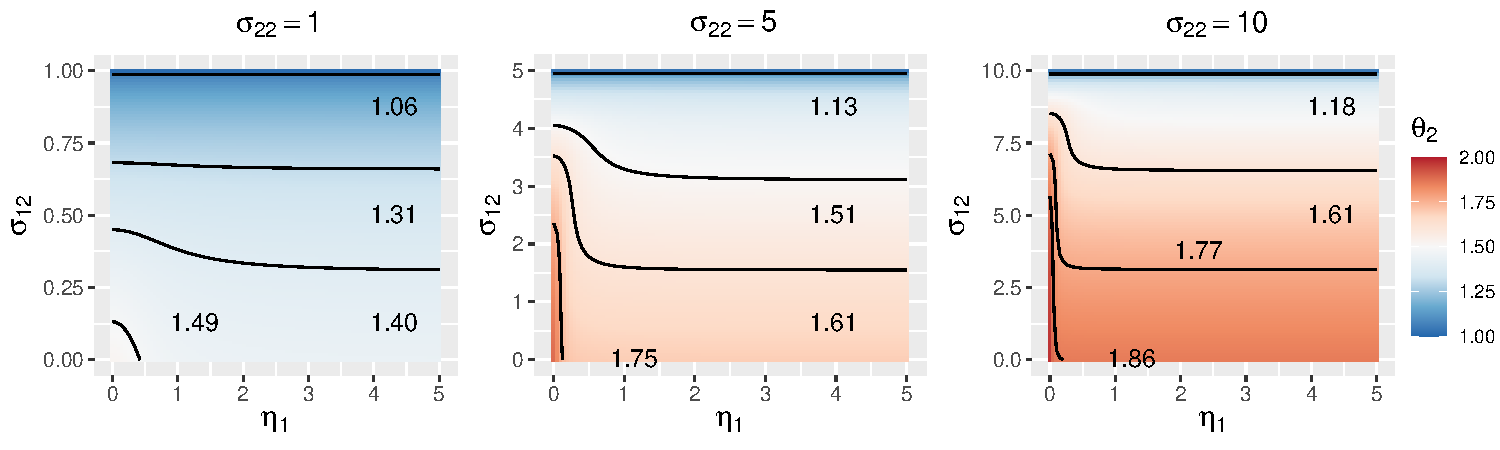
\includegraphics[width=0.95\linewidth]{bivariate_extcoef_rho_alpha.pdf}     
        \caption{}
        \label{fig:skewed_BR_extcoef}
    \end{subfigure}
    \begin{subfigure}{1\textwidth}
        \centering
        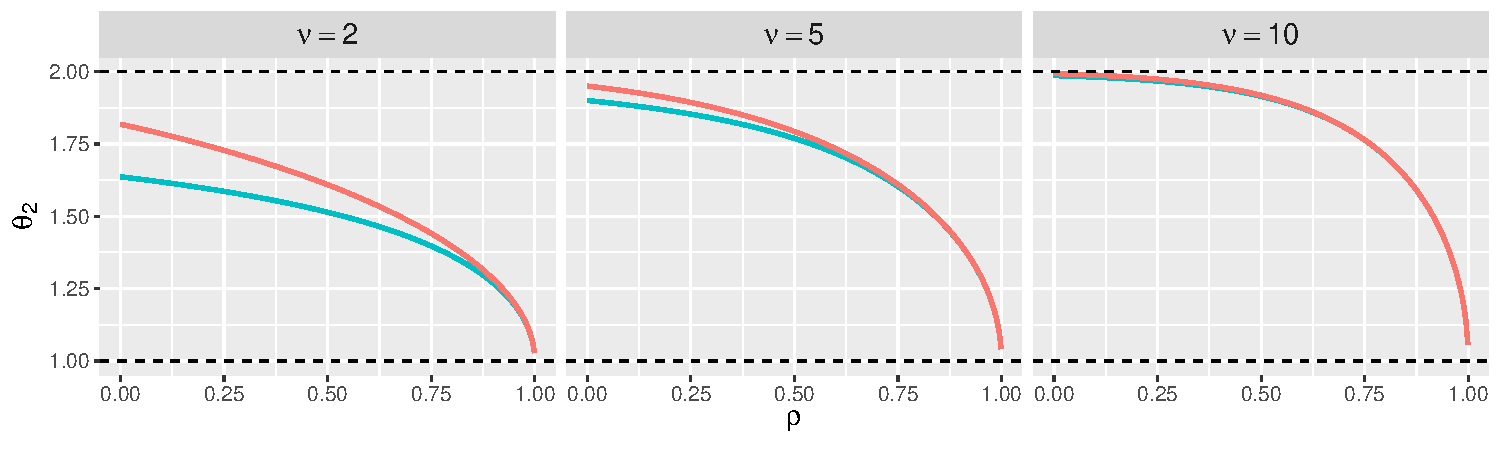
\includegraphics[width=0.95\linewidth]{bivariate_extcoef_truncT.pdf}    
        \caption{}
        \label{fig:truncated_extcoef}
    \end{subfigure}
    \caption{\small(a): Bivariate extremal coefficient of the skewed Brown-Resnick model ($\theta_2^{\textrm{sBR}}$) with $\bm\eta = (\eta_1,-\eta_1)^\top$ and $\Sigma = ((\sigma_{22},\sigma_{12})^\top,(\sigma_{12},\sigma_{22})^\top)$ where $\sigma_{22} = 1,5$ and $10$ (left to right), as function of $\eta_1$ and $\sigma_{12}$. (b): Bivariate extremal coefficient of the truncated extremal-t process ($\theta_2^{\textrm{tET}}$,blue) and the extremal-t process ($\theta_2^{\textrm{ET}}$, red) with $\nu=2,5$ and $10$ (left to right), as a function of the correlation parameter $\rho$.}
\end{figure}

% Unlike for the Brown-Resnick, t
The bivariate extremal coefficient of the skewed Brown-Resnick model only partly depends on $\Sigma$ through $\gamma_{12}$, the semivariogram of the process $Y(\bs)$ defined in Theorem~\ref{thm:skewBR}. 
%
Opting for a parametrisation based on semivariogram functions 
% over covariance functions leads to 
yields
greater interpretability of the model parameters and allows for asymptotic independence in the long range when considering an unbounded variogram. Indeed, for some spatial lag $h$, taking the power-law semivariogram with range $\lambda>0$ and  smoothness $\vartheta \in (0,2]$, i.e. $\gamma(h) = (h/\lambda)^\vartheta$,
implies that, as $h \rightarrow \infty$, $\bm \eta \equiv \bm \eta (h) \rightarrow \bm 0$ and therefore $\bm \xi = \bm \xi(h) \rightarrow \bm 0$, yielding $\theta_2 \rightarrow 2$ by \eqref{eq:bi_extcoef_skewed_BR}.
%

Estimating the $D$-dimensional parameter vector $\bm \eta$ under the constraint $\bm \eta^\top \bm 1=0$ is a 
%difficult 
task that we 
%propose to 
simplify by representing $\bm \eta$ through spline functions. Let $\eta_i = \sum_{j=1}^J b_{j}K_j(\bm s_i)$, $i=1, \ldots, D$, where $K_j(\bm s_i)$ is the $j$-th basis function evaluated at $\bm s_i = (s_{i,1}, s_{i,2})\in \calS$, and $b_j$ is the coefficient for the $j$-th basis. Imposing $\sum_{i=1}^D K_j(\bm s_i)=0$ automatically fulfills the sum-to-zero constraint for $\bm \eta$. 
%
In the remainder of this paper, $K_j(\cdot)$ denotes a Gaussian kernel centered at location $\bm s_j^\star, j=1,\dots,J$, i.e.,
\begin{equation}
\label{eq:Gaussian_splines}
    K_j(\bm s_i) = \frac{K_j^\star(\bm s_i)}{\sqrt{\sum_{k=1}^D K_j^\star(\bm s_k)^2}},    
    \quad \text{where}\quad
    K_j^\star(\bm s_i) = \phi\left(\frac{\|\bm s_i-\bm s_j^\star\|}{2\sigma_B}\right)-\frac{1}{D}\sum_{k=1}^{D}\phi\left(\frac{\|\bm s_k-\bm s_j^\star\|}{2\sigma_B}\right),
    \sigma_B>0.   
\end{equation}
%
Figure~\ref{fig:skewed_BR_extcoef_spatial} displays $\theta_2^{\textrm{sBR}}$ between locations over a $[0,32]\times[0,32]$ grid and a reference point shown as a red star, considering $\eta_i = \sum_{j=1}^2 b_{j}K_j(\bm s_i) + 0.1\text{sgn}(s_{2,i}\geq 16)$ with $J=2$ kernel centers (black dots in Figure~\ref{fig:skewed_BR_extcoef_spatial}), $\bm s_1^\star=(8,8)$ and $\bm s_2^\star=(24,24)$, and $\sigma_B = 64$. Note that $\text{sgn}(\cdot)$ denotes the sign function, which in the last term in $ \eta_i$ serves as background noise to ensure numerical identifiability of $\bm\xi = \frac{\Sigma\bm\eta}{\sqrt{1+\bm\eta^\top\Sigma\bm\eta}}$. This is because 
%when 
multiplying $\bm\eta$ by a positive constant $c$, 
%$\bm\xi=\frac{\Sigma\bm\eta}{\sqrt{1/c^2+\bm\eta^\top\Sigma\bm\eta}}$ 
will not have a numerically significant change on $\bm\xi$ as the $\bm\eta^\top\Sigma\bm\eta$ term will dominate the denominator.
\begin{figure}[!ht]
    \centering
    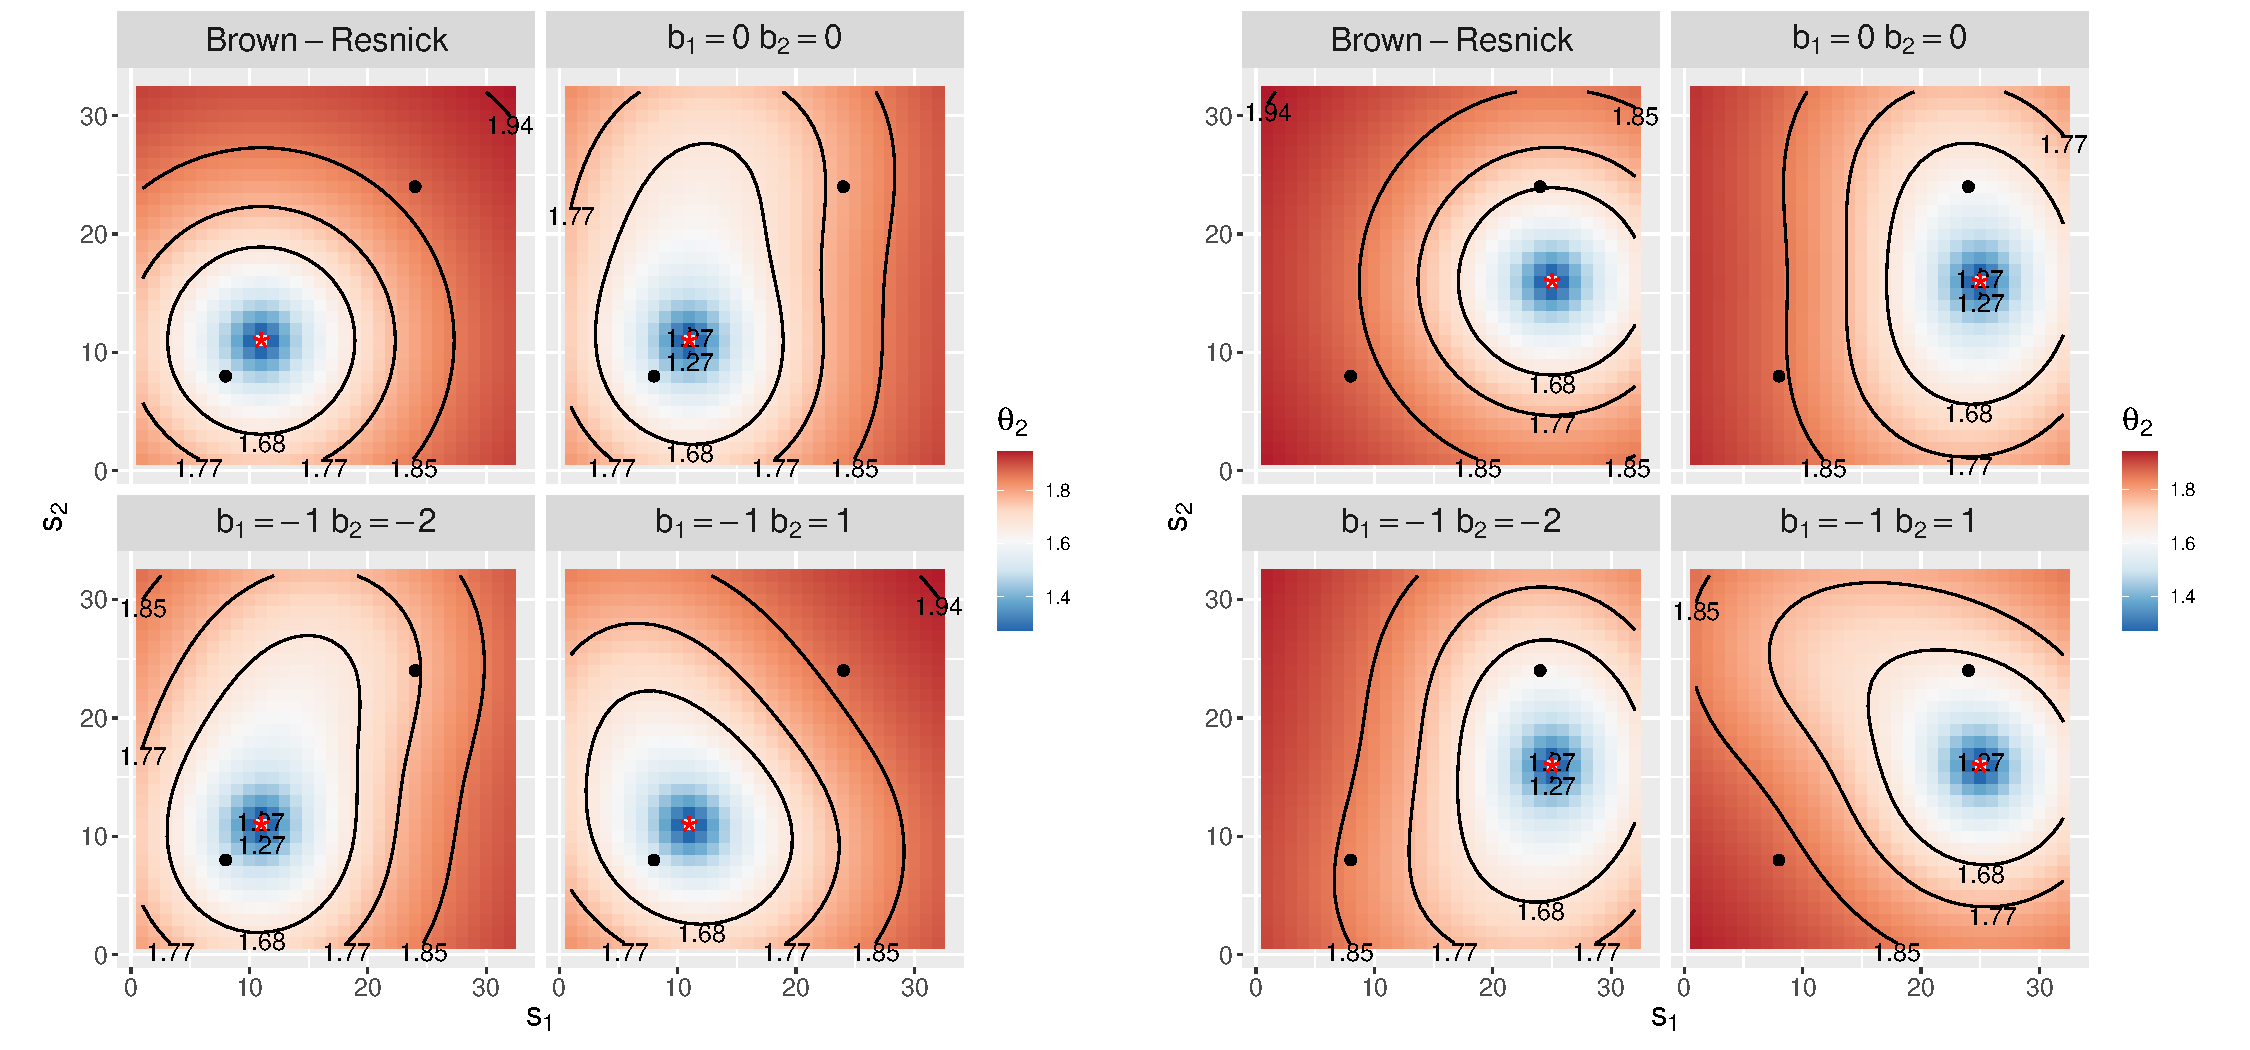
\includegraphics[width=1\textwidth]{extcoef_final_logskew.pdf}    
    \caption{\small Heatmaps and contour levels (solid black lines) of the bivariate extremal coefficient for the Brown-Resnick model ($\eta_i=0,i=1,\dots,D$) and skewed Brown-Resnick model where $\eta_i = \sum_{j=1}^2 b_{j}K_j(\bm s_i) + 0.1\text{sgn}(s_{2,i}\geq 16),i=1,\dots,D$ using $(b_1, b_2) = (0,0)$, $(-1,-2)$ and $(-1,-1)$. Black dots denote the kernel centres $\bm s_1^\star, \bm s_2^\star$. A red star indicates the reference point from which each bivariate extremal coefficient is taken with respect to.}
    \label{fig:skewed_BR_extcoef_spatial}
\end{figure}
Focusing on a single reference point (star), i.e.~on either the four left or right panels of Figure~\ref{fig:skewed_BR_extcoef_spatial}, we observe that varying the $\bm \eta$ vector through $(b_1, b_2)$ produces a broad range of dependence structures. Similarly, for fixed parameter values $(b_1,b_2)$, different dependence behaviours are observed depending on the reference point, 
%putting the spotlight on 
highlighting
an important feature of the skewed Brown-Resnick process: the ability to model non-stationarity and local anisotropy. This important property, exhibited by numerous real-world environmental extreme phenomena, is due to the fact that \eqref{eq:bi_extcoef_skewed_BR} not only depends on the spatial lag between two locations, but also on the corresponding components of the $\bm \xi$ parameter vector. A similar observation was made by \citet{Beranger.etal:2017} about the extremal skew-$t$ model.

%%%%%%%%%%%%%%%%%%%%%%%%%%%%%%%%%%%%%%%
%%%%%%%%%%%%%%%%%%%%%%%%%%%%%%%%%%%%%%%
%%%%%%%%%%%%%%%%%%%%%%%%%%%%%%%%%%%%%%%
\section{Simulation experiments}
\label{sec:sim}
%%%%%%%%%%%%%%%%%%%%%%%%%%%%%%%%%%%%%%%
%%%%%%%%%%%%%%%%%%%%%%%%%%%%%%%%%%%%%%%
%%%%%%%%%%%%%%%%%%%%%%%%%%%%%%%%%%%%%%%

%%%%%%%%%%%%%%%%%%%%%%%%%%%%%%%%%%%%%%%
%%%%%%%%%%%%%%%%%%%%%%%%%%%%%%%%%%%%%%%
\subsection{Simulation algorithms}
%%%%%%%%%%%%%%%%%%%%%%%%%%%%%%%%%%%%%%%
%%%%%%%%%%%%%%%%%%%%%%%%%%%%%%%%%%%%%%%

%Simulating from max-stable processes is a mature topic with algorithms developed for exact and conditional simulations. While the latter can be useful for predictions in the presence of constraints, we focus here on the former.
Following the approach of \citet{Dombry.Engelke.Oesting:2016},
% \citet{Dombry.Engelke.Oesting:2016} proposed an approach based on the simulation of extremal functions.
%  algorithms relying on simulation from the spectral measure \citep{Dieker.Mikosch:2015} and applied for the Brown-Resnick and extremal-$t$ models. Following this approach, \citet{Beranger.etal:2021} derives the simulation algorithm for the skewed extremal-$t$. 
% Following this approach, 
Algorithms~1 \& 2 (see Supplementary Material Sections~C.4 and D.4) describe how to randomly generate data from the skewed Brown-Resnick and truncated extremal-$t$ models. 
%
Simulating from a $r$-Pareto process 
%$\tilde{\bm Z}$ 
involves drawing from a random vector $\bm Y$ with distribution $P_{s_i}(\cdot) = \E_{\bm W}[\mathbbm 1_{\{\bm W/W(s_i)\in \cdot\}}W(s_i)]$ at a uniformly distributed random location $s_i$, where $\bm W$ is as in \eqref{eq:spectralrepresentation}, implying that
% , and such that $\bm Y/\|\bm Y\|_1$ follows the spectral distribution $\calH/D$ in \eqref{eq:decomposition} \citep[Theorem 2]{Dombry.Engelke.Oesting:2016}. 
%
%This means that simulation from $r$-Pareto models can be performed by leveraging the 
exact simulation algorithms for max-stable models can be leveraged \citep{Dombry.Engelke.Oesting:2016,Dombry.etal:2024}.  
%
%For the extremal-$t$ process, \citet[][Proposition~5]{Dombry.Engelke.Oesting:2016} shows that $\max(\bm T,0)^\nu$, where $\bm T$ follows the multivariate Student-$t$ distribution with $\nu+1$ degrees of freedom, follows the distribution $P_{s_i}$, confirming the presence of mass on the boundaries. 

When the risk functional is the $L_1$ norm, i.e., $r_0(\cdot)=\|\cdot\|_1$, $r$-Pareto samples can be simply obtained as $\tilde R\bm Y/\|\bm Y\|_1$, where $\tilde R$ follows a unit Pareto distribution.  
For another risk functional $r_1(\cdot)$, let $M$ be such that
%a constant bounding $r_1$ from above with the $L_1$ norm, i.e., 
$r_1 (\cdot) \leq Mr_0 (\cdot)$.
%
Samples for the $r$-Pareto process with risk functional $r_1(\cdot)$ can then be obtained by 
sampling $\bm{\tilde Z}$
%applying rejection sampling to the samples 
from the process with risk functional $r_0(\cdot)$, 
and accepting a sample 
%where a sample is accepted 
as $\bm{\tilde Z}/M$ when $r_1(\bm {\tilde Z})\geq M$ \citep[Proposition 2]{Dombry.etal:2024}.
% 
% \citet[Proposition 2]{Dombry.etal:2024} introducesa a constant $M$ bounding $r_1$ from above, with the $L_1$ norm, i.e., $r_1 (\cdot) \leq Mr_0 (\cdot)$.
 % , where $r_1$ is another risk functional than the $L_1$ norm . 
% The constant $M$ is used to bound the risk functional $r_1$ from above, with the $L_1$ norm. 
% Practically, simulation from the $r$-Pareto process with the $L_1$ norm as risk functional is first performed and rejection sampling is then applied to derive samples from the $r$-Pareto process with another risk functional, where a sample is accepted as $\bm{\tilde Z}/M$ when $r_1(\bm {\tilde Z})\geq M$. 
The constant $M=1$ when $r_1 =\|\cdot\|_\infty $ and $M=D^{p-2}$ when $r_1 = \|\cdot\|_p$, $p>1$.

Larger $M$ implies lower acceptance probabilities. 
%in the rejection sampling step and thus higher computational cost of the algorithm. 
However, note that for a convex risk functional $r(\cdot)$, e.g., $L_p$ norm, $p\geq 1$, the support space $\calA_r \in \mathbb R_+^D$ has complement $\calA_r^c=\{\bm x\in\mathbb R_+^D: r(\bm x)\leq 1\}$, which is a convex set. Hence $\calA_r\subset \calA_{r_0}$. Following from this, an efficient simulation algorithm for a $r$-Pareto process with any convex risk functional $r(\cdot)$ is given below (see Supplemental Material~E.1 for a proof). 
%    
\begin{theorem}\label{thm:r_pareto_simulation}
Let $\bm{\tilde Z}^{(r_0)}$ be a $r$-Pareto random vector at $D$ locations with risk functional $r_0(\cdot)=\|\cdot\|_1$. Let $r(\cdot)$ be any convex risk functional, homogeneous of order 1, such that $r(\bm 0)=0$ and $r(\bm e_i)=1/c_i>0, i=1,\dots,D$, where $\bm e_i$ are standard basis vectors of dimension $D$.
%
% Let $r(\cdot)$ be any risk functional that is convex, homogeneous of order 1, and such that $r(\bm 0)=0$. Suppose $r(\bm e_i)=1/c_i>0, i=1,\dots,D$, where $\bm e_i$ are the basis vectors of dimension $D$, and $\bm{\tilde Z}^{(r_0)}$ is the $r$-Pareto process at $D$ locations with risk functional $r_0(\cdot)=\|\cdot\|_1$. 
The r-Pareto process with risk functional $r(\cdot)$ can be simulated as $\bm{\tilde Z}^{(r)}\eqd c_0\bm{\tilde Z}^{(r_0)}\ | \ r\left(\bm{\tilde Z}^{(r_0)}\right) > 1/c_0$, where $c_0 = \min\{\min_{i=1}^D c_i,1\}$.
\end{theorem}
%
For example, considering $r(\cdot)=\|\cdot\|_p,\ p>1$ gives $1/c_0 = 1$ instead of $M=D^{p-2}$ in \citet{Dombry.etal:2024}, while $r(\bm x)=\sum_{i=1}^D m_ix_i, m_i\in [0,\infty],i=1\dots,D$, a linear convex combination, produces $c_0=\min\{\min_{i=1}^D 1/m_i,1\}$. This algorithm is simpler than the one proposed by \citet[Proposition 1]{Dombry.etal:2024} when $r(\cdot)$ is a linear convex combination. Table~\ref{tab:simu_exceedances_p_d} shows the acceptance rate of both algorithms, when generating samples for a Brown-Resnick $r$-Pareto process with a $L_p$ risk functional, $p=2,3,5,10$, for varying dimension $D$. 
%
As $p$ increases, the acceptance rate decreases quickly to zero using method in \citet{Dombry.etal:2024}, especially when $D$ is large. In contrast, our method achieves a comparable or higher acceptance rate
%, that is at least $10\%$ 
in all cases, particularly for $p>2$.   
%
However the approach of \citet{Dombry.etal:2024} is more general and can be used when $r(\cdot)$ is not convex, but homogeneous of order 1 (e.g., $r$ returns any order statistics excluding the maximum), once $M$ has been obtained. \PZ{Though we are not investigating inference for $r$-Pareto models with risk functionals other than $L_1$ norm, which is out of scope of this paper, it is also possible to construct tractable likelihood based inference for $r$-Pareto models with other risk functional. For example, for $r(\bm x) = x_0$, we have 
$$\bm{\tilde Z}^{(r)} - \bm{\tilde Z}^{(r)}_0 \bm 1\ |\ r(\bm{\tilde Z}^{(r)}) = \bm{\tilde Z}^{(r)}_0 > 1 \sim P_{s_0}(\cdot),$$ 
which can be used to conduct likelihood inference for extremes conditioning on a single site being extreme.}

% In the following simulations, Theorem \ref{thm:r_pareto_simulation} is used to randomly generate data, and is also leveraged in our proposed inference methodology (see Section~\ref{sec:inference}).

\begin{table}[ht]
    \centering
    \caption{\small Percentage of samples from $10^5$ Brown-Resnick $r$-Pareto processes replicates with $L_1$ risk functional that fall into the acceptance region for $r(\cdot)$ being $L_p,p=2,3,5,10$, using the methods in \citet{Dombry.etal:2024} (left number in each cell) and Theorem~\ref{thm:r_pareto_simulation} (right number). Dimension is $D=4,16,64,100$ and dependence structure is defined via a power-law semivariogram $\gamma(h)=h/\lambda$, $\lambda=2$, on the grid $[1,\sqrt{D}]^2$.}
    \begin{tabular}{lccccc}
    $L_p/D$ & \phantom{$>$}$D=4$ & \phantom{$>$}$D=16$ & $D=64$ & $D=100$ \\
    \hline
    $p=2$ & \phantom{$>$0.}59/59 & \phantom{$>$0.}37/37 & \phantom{0.}25/25 & \phantom{0.}22/22\\
    $p=3$ & \phantom{$>$0.}13/52 & \phantom{$>$}1.80/29 & 0.27/18 & 0.19/16\\
%    $p=5$ & \phantom{>}0.76/49 & 0.006/26 & 0/16 & 0/14\\
     $p=5$ & \phantom{$>$}0.76/49 & $>$0.01/26 & 0.00/16 & 0.00/14\\
%    $p=10$ & 0.001/47 & 0.000/25 & 0.0/15 & 0/13\\
    $p=10$ & $>$0.01/47 & \phantom{$>$}0.00/25 & 0.00/15 & 0.00/13\\
    \hline
\end{tabular}
    \label{tab:simu_exceedances_p_d}
\end{table}

%%%%%%%%%%%%%%%%%%%%%%%%%%%%%%%%%%%%%%%
%%%%%%%%%%%%%%%%%%%%%%%%%%%%%%%%%%%%%%%
\subsection{Parameter estimation}
\label{ssec:par_est}
%%%%%%%%%%%%%%%%%%%%%%%%%%%%%%%%%%%%%%%
%%%%%%%%%%%%%%%%%%%%%%%%%%%%%%%%%%%%%%%

%%%%%%%%%%%%%%%%%%%%%%%%%%%%%%%%%%%%%%%
\subsubsection{Spectral vs pairwise composite likelihoods}
%%%%%%%%%%%%%%%%%%%%%%%%%%%%%%%%%%%%%%%

An initial experiment on the Brown-Resnick model (Supplementary Material~F) 
% where $500$ samples are generated from the Brown-Resnick model in large dimension ($D=225$) 
indicates that, unlike the composite likelihood, the spectral likelihood produces biased estimates especially with weaker dependence, supporting the findings from \citet{Engelke.etal:2015, Huser.etal:2016}. 
However, the pairwise likelihood 
%outperforms the spectral likelihood for this model, it is computationally expensive and 
is around $476$ times slower to implement.
% Although the pairwise likelihood method is unbiased for Brown-Resnick processes, it is computationally expensive and, in this scenario, about $476$ times slower than the spectral likelihood. 
%

For our new models, composite likelihood is not directly applicable for truncated extremal-$t$ \PZ{models} as the marginal distribution of a multivariate truncated normal is not truncated normal, and the actual density requires a costly numerical integration for each composite likelihood term \citep{Horrace:2005}. 
% Moreover, for skewed Brown-Resnick processes, this approach yields unreliable estimates of the skewness parameters $b_1$ and $b_2$
%the pairwise likelihood estimators for the skewness parameter $b_1$ and $b_2$ are found unreliable.
%
% To illustrate this point, 
We therefore focus on the skewed Brown-Resnick model \PZ{with power-law semivariogram}  defined on a $15\times15$ grid  ($D=225$) with parameters $\lambda=3$, $\vartheta=1$, and $(b_1,b_2) = (-1,-2)$, where the centres of the kernels are 
%chosen to be 
$\bm s_1^\star = (4,4)$ and $\bm s_2^\star=(11,11)$, and consider samples of size $n=500$. 
%
The threshold for the spectral likelihood \eqref{eq:angular_likelihood_1} is set at $u = 30 \times D$ and the composite likelihood weights in 
%the composite likelihood 
\eqref{eq:composite} are set to 0/1 to
%realise a cut-off distance to 
only include the $1,202$ closest pairs, mitigating computational complexity.
% 
%After replicating the estimation procedure $300$ times (as for all upcoming experiments), v
Violin plots of the estimates (for 300 replicate analyses) are displayed in Figure~\ref{fig:simulation_boxplot_skewedBR_comp}, demonstrating almost unbiased estimates for $b_1$ and $b_2$ and small relative bias (${\sim}10\%$) for $\lambda$ and $\vartheta$ when the spectral likelihood (red) is applied. 
%
In contrast, the pairwise likelihood estimates (blue) for $\lambda$ and $\nu$ are unbiased, but those for $b_1$ and $b_2$ are biased and almost unreliable, which may be attributed to the inability of this approach to capture the locally anisotropic dependence structure 
% presented in 
of the data. The spectral likelihood is about $68$ times faster than the composite likelihood, taking $124$ seconds on a $16$-core machine (as for all computations in this manuscript) and considering multiple initial values for the skewness parameter to avoid local maxima.  
%
\begin{figure}[!ht]
    \centering
    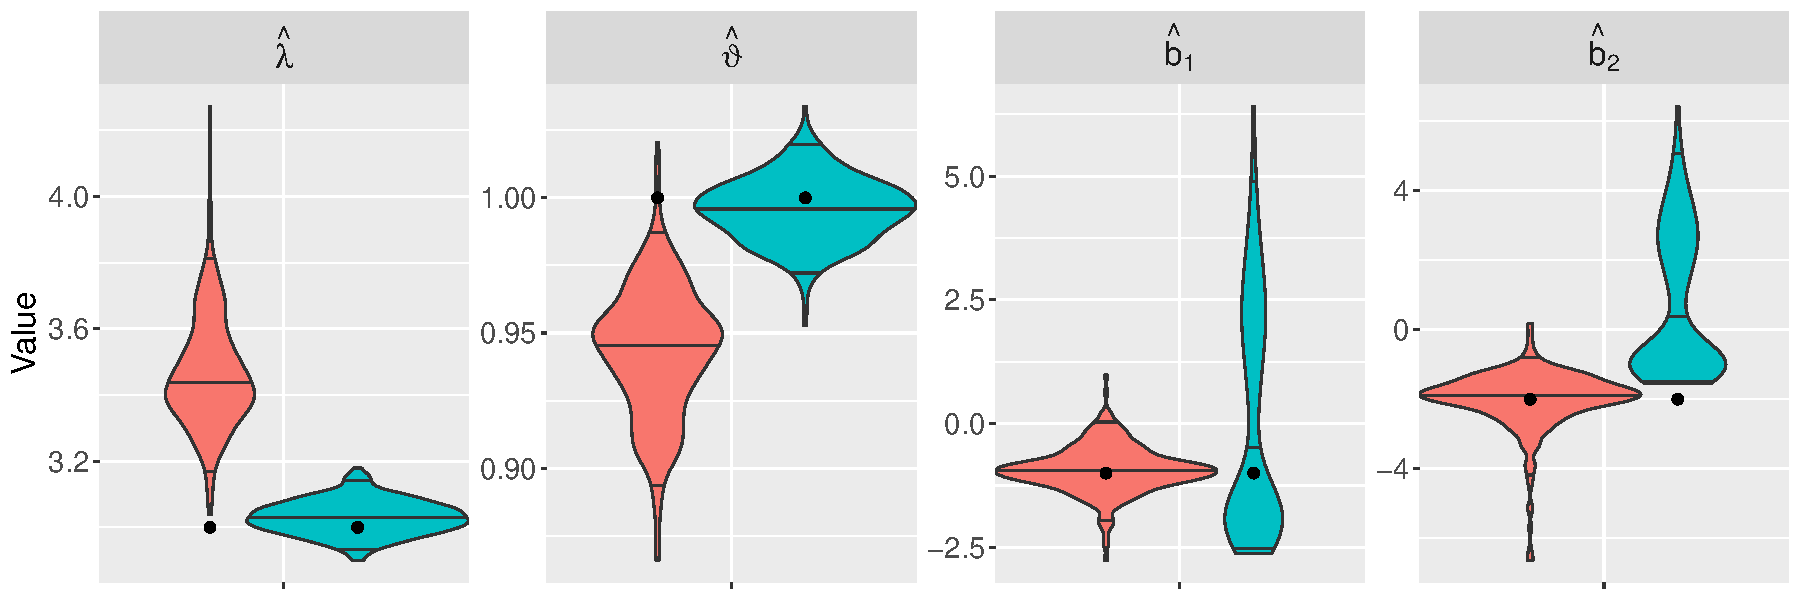
\includegraphics[width=0.95\textwidth]{simulation_est_boxplots_final_skewBR_comp.pdf}
    \caption{\small Violin plots for 300 estimates of $\bm \theta = (\lambda, \vartheta, b_1, b_2)$ for the skewed Brown-Resnick process with $\lambda=3$, $\vartheta=1$, and $(b_1,b_2) = (-1,-2)$ using the spectral likelihood (red; left) with threshold $u=30\times D$ and the pairwise likelihood (blue; right) with 1,202 pairs. Black dots indicate the true values.}
    \label{fig:simulation_boxplot_skewedBR_comp}
\end{figure}
%   

%%%%%%%%%%%%%%%%%%%%%%%%%%%%%%%%%%%%%%%
\subsubsection{Threshold selection for spectral likelihoods}
%%%%%%%%%%%%%%%%%%%%%%%%%%%%%%%%%%%%%%%

%When fitting models using the spectral likelihood, the question of selecting an appropriate threshold $u$ arises.
%While the answer is not trivial, some insights can be drawn by the following experiments.

First, we consider the skewed Brown-Resnick model with sample size 
%increased to 
$n=2000$ and all 12 parameter combinations from $\lambda=5,10$, $\vartheta = 1,1.5$, and $(b_1,b_2) = (0,0),(-1,-2),(-1,1)$. The grid size and kernel centres remain unchanged. The threshold in the spectral likelihood is set as $u=100\times D$, retaining the ${\sim}20$ observations with largest radial component.
%, a figure roughly equivalent to the previous experiment. 
Figure~\ref{fig:simulation_boxplot_skewedBR} displays violin plots for each parameter estimate and true parameter combination (indicated as cases $1-12$), highlighting that all parameters were accurately identified, no matter the degree of dependence. This confirms that increasing $u$ reduces bias in the spectral likelihood since the Poisson approximation is better. 
%Finally, note that m
Model fitting is computationally efficient, taking on average ${\sim}6$ minutes per fit using 16 cores and setting multiple initial values for the skewness parameter.
%
\begin{figure}[!ht]
    \centering
    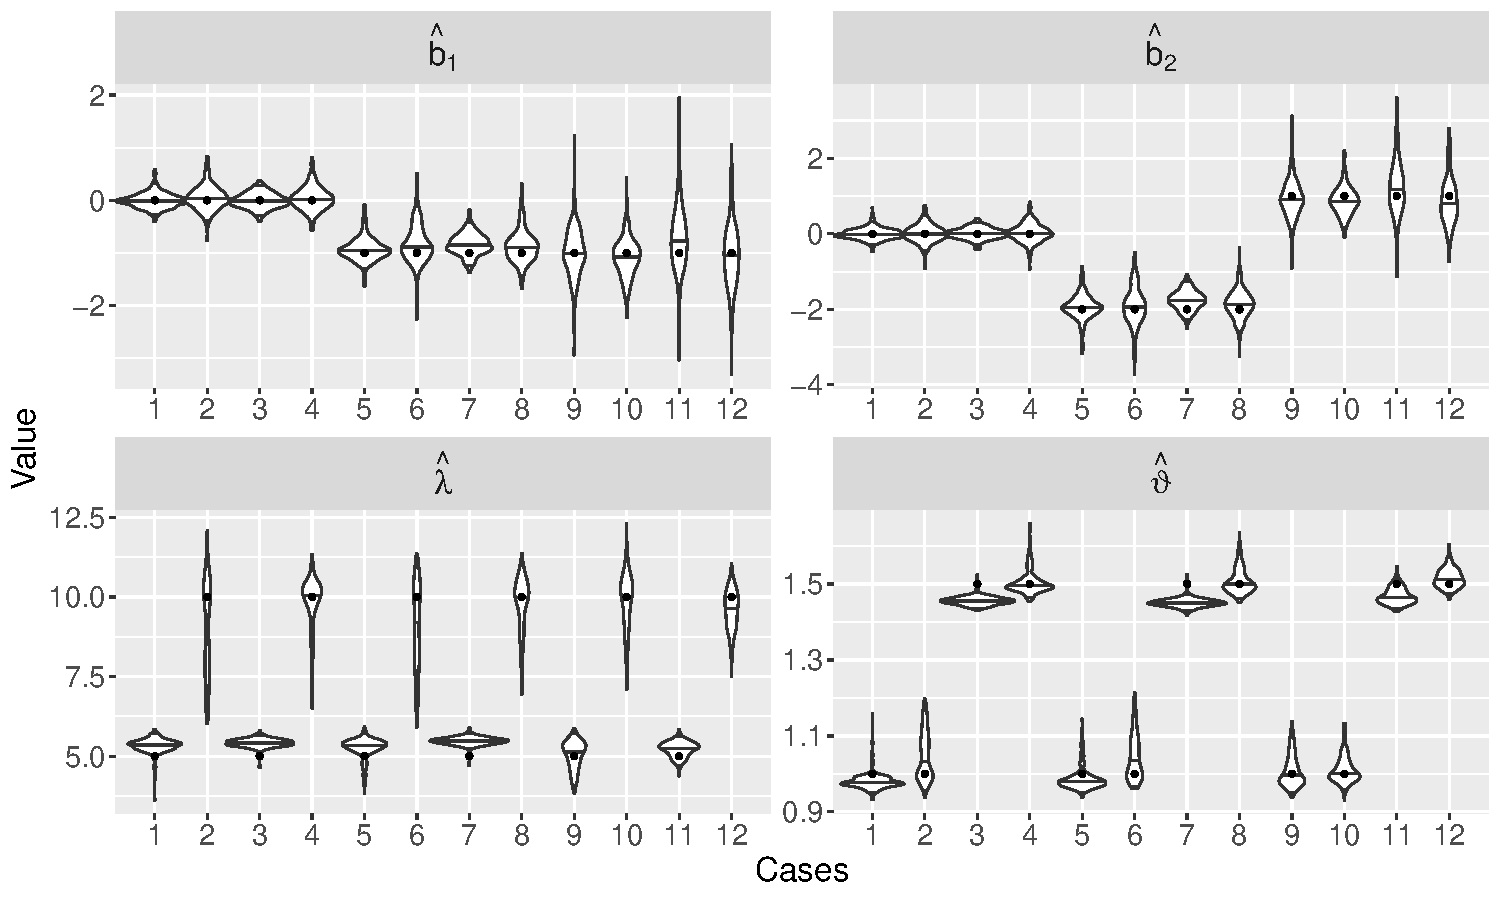
\includegraphics[width=0.95\textwidth]{simulation_est_boxplots_final.pdf}    
    \caption{\small Violin plots for the 300 estimates of $\bm \theta= \left(\lambda, \vartheta,  b_1, b_2\right)$ for the skewed Brown-Resnick process with all combinations of $\lambda=5,10$, $\vartheta=1,1.5$, and $(b_1,b_2) = (0,0),(-1,-2),(-1,1)$, using the spectral likelihood. Black dots indicate the true values.}
    \label{fig:simulation_boxplot_skewedBR}
\end{figure}
%

We now generate $n=2000$ samples from the truncated extremal-$t$ model \PZ{with correlation function $\rho(h) = \exp\{- (h/\lambda)^\vartheta\}$} defined on a $10\times10$ grid ($D=100$) 
% where $2000$ samples are generated from 
with 2 parameter combinations using $\lambda=3, 5$, $\vartheta=1$ and $\nu=2$.
%
% Spectral likelihood estimation is performed while 
Fixing 
%the degree of freedom to its true value, 
$\nu=2$, 
%spectral likelihood estimation is performed with results presented in 
Figure~\ref{fig:simulation_boxplot_truncT} shows the results of spectral likelihood estimation
where the threshold $u$ is set as the $98\%$ (red), $95\%$ (green), and $90\%$ (blue) quantiles of the observed radial components.
% The spectral likelihood is again fitted where the degree of freedom is fixed to its true value ($\nu=2$). 
% Figure~\ref{fig:simulation_boxplot_truncT} displays violin plots of the estimates $\hat{\lambda}$ and $\hat{\vartheta}$ when the threshold $u$ is set as the $98\%$ (red), $95\%$ (green), and $90\%$ (blue) quantiles of the observed radial components.
%
% For a sample size $n=2000$, 
Retaining the $40$ ($u=98\%$) observations with largest radial components produces almost unbiased estimates. Lowering $u$ increases the bias but also increases computation time since more observations are included. As noted in Section~\ref{ssec:new_models}, fitting the truncated extremal-$t$ model requires more computational effort than the skewed Brown-Resnick, taking on average ${\sim}15$ minutes.   
%
Overall, 
%it is recommended to select a 
a threshold should be as high as possible while retaining enough observations to control estimate variability.
%the variability of the estimates.
%
\begin{figure}[!ht]
    \centering
    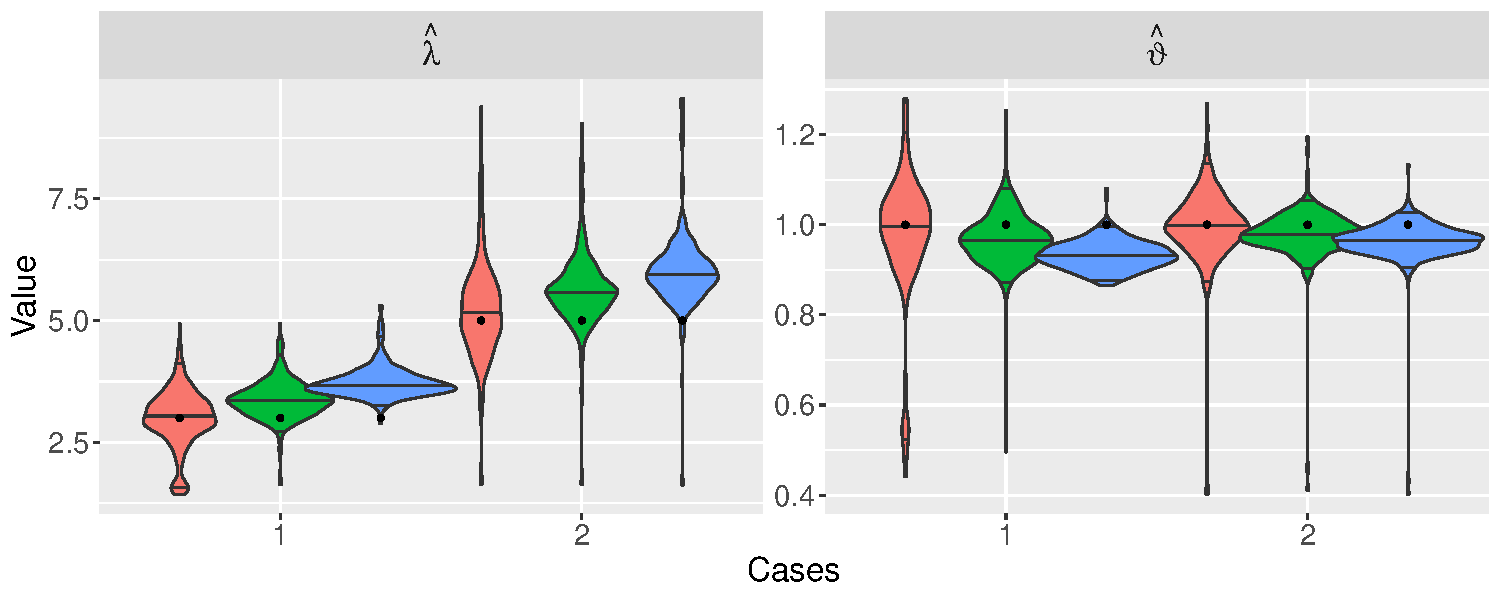
\includegraphics[width=0.95\textwidth]{simulation_est_boxplots_final_truncT.pdf}    
    \caption{\small Violin plots for the spectral likelihood estimates of the truncated extremal-$t$ model with $\lambda=3,5$, $\vartheta=1$, and $\nu=2$ (fixed), and threshold $u$ set as the $98\%$ (red), $95\%$ (green) and $90\%$ (blue) empirical quantiles of the radial component. Black dots indicate the true parameter values.}
    \label{fig:simulation_boxplot_truncT}
\end{figure}
%

%%%%%%%%%%%%%%%%%%%%%%%%%%%%%%%%%%%%%%%
\subsubsection{Spectral likelihoods vs score matching}
%%%%%%%%%%%%%%%%%%%%%%%%%%%%%%%%%%%%%%%

We now compare the performance of the spectral likelihood to the popular score matching approach \citep[see][]{deFondeville.Davison:2018} when fitting $r$-Pareto processes with different risk functionals.
% The interest is now in fitting $r$-Pareto processes with different risk functionals and investigating the performance of the spectral likelihood over the well-adopted score matching approach \citep[see][]{deFondeville.Davison:2018}. 
%
We sample $n=2,000$ observations from the skewed Brown-Resnick $r$-Pareto process defined on a $15\times15$ grid with the same parameter combinations as in Figure~\ref{fig:simulation_boxplot_skewedBR} and taking the $L_1$ as the risk functional. An observation is considered extreme when exceeding the 
%threshold $u$ which selected as the $
$95\%$ empirical quantile of $r(\bm X_1),\dots,r(\bm X_n)$.

%Estimation outputs 
\PZ{Estimates of $\vartheta$ and $b_1$ are shown in Figure~\ref{fig:simulation_boxplot_rpareto_skewedBR}. }
%for $\hat{\vartheta}$ and $\hat{b}_1$ 
(Estimates for $\hat{\lambda}$ and $\hat{b}_2$ are reported in Figure~2 of Supplementary Material~E.3.)
%
%Across all dependence structure regimes, t
The spectral likelihood consistently provides unbiased, low variability estimates (blue) for all 
%four 
parameters
%, and with low variability, 
across all dependence structure regimes. 
%
%Comparatively, 
In contrast, score matching produces unbiased but more variable estimates (red) 
%of both parameters 
and can become
% On the contrary, although the score matching approach is able to produce unbiased but more variable estimates (red) of $\lambda$ and $\vartheta$, it becomes 
numerically unstable for the skewness parameters (e.g., cases 7--12).
% 
%On top of being more statistically efficient, 
The spectral likelihood is also more computationally efficient, being ${\sim}5$ times faster than the score matching approach (141 versus 726 seconds on average using 3 CPU cores). 
%
\PZ{Figures~3 report similar results and conclusions for the truncated extremal-$t$ $r$-Pareto process with $L_1$ norm risk functional.}

%
% \begin{figure}[ht]
%     \centering
%     \includegraphics[width=1\textwidth,page=2]{simulation_pareto_violin__5_Inf_Inf.pdf}    
%     \caption{Violin plots for the score matching (left) and spectral likelihood (right) estimates of $\bm \theta= \left(\lambda, \vartheta,  b_1, b_2\right)$ for the skewed Brown-Resnick $r$-Pareto process with $L_3$ norm risk functional and the same parameter combinations as in Figure~\ref{fig:simulation_boxplot_skewedBR}. Black dots indicate the parameter true values. \textcolor{red}{Need to improve the quality of those plots.}}
%     \label{fig:simulation_boxplot_rpareto_skewedBR}
% \end{figure}
\begin{figure}[ht]
    \centering
    \includegraphics[width=0.95\textwidth,page=2]{simulation_pareto_violin_logskew_5.pdf}
    \includegraphics[width=0.95\textwidth,page=3]{simulation_pareto_violin_logskew_5.pdf}
    \caption{\small Violin plots for score matching (red) and spectral likelihood (blue) estimates of $\vartheta$ (top) and  $b_1$ (bottom) for the skewed Brown-Resnick $r$-Pareto process with $L_1$ norm risk functional and the same parameter combinations as in Figure~\ref{fig:simulation_boxplot_skewedBR}. Black dots indicate the parameter true values.}
    \label{fig:simulation_boxplot_rpareto_skewedBR}
\end{figure}
%
% Experiments on the truncated extremal-$t$ $r$-Pareto process 
% % are also conducted on a $8\times8$ grid with $8$ parameter combinations, and 
% presented in Figure~4 of the Supplementary Material.

In conclusion, 
% the above experiments indicate that 
the spectral likelihood is a statistically and computationally efficient methodology that can infer the model parameters of max-stable and $r$-Pareto processes. 
% especially for the newly introduced skewed Brown-Resnick and truncated extremal-$t$ models. 
For max-stable processes, a carefully selected threshold 
%$u$ 
will 
%allow to 
control the bias in the estimates due to the Poisson approximation.
There is no bias (or approximation) for $r$-Pareto processes.
%while for $r$-Pareto processes this approximation does not exist and yielding unbiased estimates with small variance. 
The computational gains are significant, which enables the tackling of higher dimensional problems.

%%%%%%%%%%%%%%%%%%%%%%%%%%%%%%%%%%%%%%%
%%%%%%%%%%%%%%%%%%%%%%%%%%%%%%%%%%%%%%%
%%%%%%%%%%%%%%%%%%%%%%%%%%%%%%%%%%%%%%%
\section{Practical applications}
\label{sec:real}
%%%%%%%%%%%%%%%%%%%%%%%%%%%%%%%%%%%%%%%
%%%%%%%%%%%%%%%%%%%%%%%%%%%%%%%%%%%%%%%
%%%%%%%%%%%%%%%%%%%%%%%%%%%%%%%%%%%%%%%

%%%%%%%%%%%%%%%%%%%%%%%%%%%%%%%%%%%%%%%
%%%%%%%%%%%%%%%%%%%%%%%%%%%%%%%%%%%%%%%
\subsection{Analysis of extreme rainfall over Florida}
%%%%%%%%%%%%%%%%%%%%%%%%%%%%%%%%%%%%%%%
%%%%%%%%%%%%%%%%%%%%%%%%%%%%%%%%%%%%%%%

We analyse the spatial dependence structure rainfall across the Tampa Bay area, Florida, during the wet season (June--September).
%is investigated. 
The data comprise radar measurements recorded at 15 minute intervals between 1995--2019, over a regular 2km grid. The dataset is made of $n=139,881$ radar images with $4,449$ spatial observations in each image.
%
\cite{deFondeville.Davison:2018} fitted a Brown-Resnick $r$-Pareto process to these data restricted to the 1999--2004 period and $3,600$ locations. 
%
%The same fitting procedure is applied here as benchmark to demonstrate the advantages of using the spectral likelihood. 
To motivate the need for a broader class of models, we fit the skewed Brown-Resnick model with spline representation of $\bm\eta$ as in Section~\ref{ssec:flex_dep} with four kernels (see black dots in Figure~\ref{fig:extcoef_application_florida}) to the full dataset.
%
As a pre-processing step, the data are marginally transformed to unit Pareto scale using the empirical distribution function, while zero values are ignored and treated as missing. 
%
We adopt an anisotropic semivariogram function
%
\begin{equation}
    \label{eq:semivar}
    \gamma(\bm h) = \left(\frac{\left\| V \bm h\right\|_2}{\lambda}\right)^\vartheta, \:\vartheta\in(0,2],\:\lambda>0,
\end{equation}
%
where $\bm h$ is the difference vector between coordinates of two locations and 
%
\begin{equation*}
\label{eq:aniso_mat}
    V = \begin{pmatrix}
    \cos\zeta & - \sin\zeta\\
    m\sin\zeta &  m\cos\zeta
    \end{pmatrix},\: m >0 , \:\zeta\in (-\frac{\pi}{4},\frac{\pi}{4})
\end{equation*}
is a matrix used to capture the global anisotropy in the dependence structure.
%
\PZ{The $r$-Pareto processes are defined using the $L_1$ norm as the risk functional, %These choices are 
which selects events with high cumulative rainfall over the whole region.} 
% Although these types of events are of different nature, both can lead to flooding and both have recently occurred in Florida. For example, a plume of moisture caused heavy rainfall in southern Florida on June 11, 2024 generating high risks of localised flash flooding \citep{doermann2024rainfall}, whereas hurricanes Irma and Milton (September 2017 and October 2024) lasted several days and touched large parts of the state \citep{cangialosi2021irma, beven2025milton}. 
%
To choose the thresholds, a univariate generalized Pareto distribution is fitted to the values of the corresponding risk functional evaluated at each observations and the level for which the estimated shape parameter becomes stable is selected. 
%
%As a result, the threshold $u$ is set as the 
This produces a threshold set at the $99.95\%$ empirical quantile of $\{r(\bm X_i)\}$
%$,\dots,r(\bm X_n)$ 
for both 
% $L_1$ and $L_\infty$ norm 
risk functionals, leaving $70$ 
%most extreme 
observations for model fitting. 
%
% Averaging the computation times for both risk functions, the skewed Brown-Resnick and Brown-Resnick $r$-Pareto models are fitted using the spectral likelihood in about 8.00 and 0.85 hours respectively, with a 16-core machine. Such difference in computing time is simply due to the model complexity, the skewed Brown-Resnick having an additional $4$ parameters.
% 

\PZ{Table~\ref{tab:parameter_estimates} reports parameter and standard error estimates for both skew (sBR) and standard (BR) Brown-Resnick models. The range parameter ($\lambda$) estimates are given in km/unit. For the Brown-Resnick models, spectral likelihood (BR) and score-matching (BR$^{sm}$) produce broadly consistent parameter estimates, although score matching produces notably smaller estimates of the range parameter $\lambda$. Figure~4 of the Supplementary Material shows the extremal coefficients of the Brown-Resnick model for both inference approaches, which strongly suggests the range parameter estimates using score matching are underestimated. Similar to Section~\ref{ssec:par_est}, using the spectral likelihood is respectively $80\%$ faster than score matching. 
%
Inference for the sBR requires greater computation, reflecting its $4$ additional parameters. 
% All computation reported in this section and the next one are performed on a 16-core machine.
}

\begin{table}[!ht]
    \centering
    \scalebox{0.85}{
        \begin{tabular}{lcccccccccccc}
            \hline
           Model & % $r(\cdot)$ &
           $\hat\lambda$ & $\hat\vartheta$ & $\hat\zeta$ & $\hat m$ & $\hat b_1$ & $\hat b_2$ & $\hat b_3$ & $\hat b_4$ & \textrm{Time (hrs)} & \textrm{AIC}\\ 
            \hline                
            $\textrm{BR}^{sm}$ &  2.80 & 1.40 & -0.12 & 1.06 & - & - & - & - & 2.05 & -\\ 
              & & (0.25) & (0.09) & (1.25) & (0.07) & - & - & - & - \\
            BR & 5.91 & 1.16 & -0.73 & 0.96 & - & - & - & - & 1.14 &  173459.5 \\ %2485.88\\ 
              & & (1.71) & (0.11) & (1.21) & (0.07) & - & - & - & - \\ 
            % $\textrm{BR}^{sm}$ & $L_\infty$ & 3.49 & 1.71 & -0.04 & 1.02 & - & - & - & - & 1.90 & -\\ 
            %   & & (0.22) & (0.04) & (1.83) & (0.05) & - & - & - & - \\   
            % BR & $L_\infty$ & 6.30 & 1.37 & 0.40 & 0.95 & - & - & - & - & 1.70 & 176311.0 \\% 2526.61 \\ 
            %   & & (0.39) & (0.03) & (0.36) & (0.04) & - & - & - & - \\ 
            sBR &  5.81 & 1.19 & 0.73 & 1.04 & 11.39 & 8.58 & 23.09 & 19.89 & 4.20 & 172663.1 \\ %2482.39\\ 
              & & (1.74) & (0.11) & (2.83) & (0.15) & (27.15) & (21.37) & (56.21) & (47.90) \\ 
            % sBR & $L_\infty$ & 5.96 & 1.41 & 0.46 & 0.96 & 0.16 & 0.15 & 0.06 & 0.07 & 4.94 & 174626.6 \\ %2510.44\\ 
            %   & & (0.35) & (0.03) & (0.28) & (0.04) & (1.22) & (1.22) & (0.52) & (0.48) \\ 
            \hline
        \end{tabular}
    }
    \caption{\small Spectral likelihood parameter estimates (with jackknife estimates of standard errors) for the Brown-Resnick (BR) and skewed Brown-Resnick (sBR) $r$-Pareto models with $L_1$ norm risk functional. 
    %Model name with 
    %An asterisk ($^*$) 
    The superscript $sm$ indicates inference performed using score matching.}
    \label{tab:parameter_estimates}
\end{table}

Focusing on the spectral likelihood results,
%Comparing the model fits using the spectral likelihood indicates 
there is no evidence against $m=1$, implying that there is no global anisotropy in the dependence structure, a finding consistent with \cite{deFondeville.Davison:2018}. 
%
The standard errors of 
% the slant parameters 
$b_1,\ldots,b_4$ are relatively large, and although confidence intervals include zero, this does not imply there is no evidence these parameters are non-zero. 
Indeed, unlike in Section~\ref{ssec:par_est}, no background noise has been added since only $\bm \xi$ needs to be estimated (instead of $\bm \eta$) and the identifiability of $b_1, \ldots, b_4$ is not a concern but reflected in the jackknife estimates of the standard errors.
% in the representation of the $\bm \eta$ parameter and therefore identifiability issues are reflected in the jackknife estimates of the standard errors.
%
The greater flexibility offered by the skewed Brown-Resnick is demonstrated by lower AIC values, which is based on the spectral likelihood, 
%of the Akaike Information Criterion (AIC) 
for both risk functions.
%(respectively $2482.39$ against $2485.88$ and $2510.44$ against $2526.61$). 
Preference for the sBR model indicates that a local anisotropic dependence structure is detected.

 


%
Figure~\ref{fig:extcoef_application_florida} provides maps of empirical bivariate extremal coefficients (shading) with respect to two different reference points (south-west, north-west). We note that the empirical extremal coefficient patterns appear to vary with the reference location, indicating a non-stationary dependence structure. The ability of the sBR model (and the inability of the BR model) to capture these local dependence features can be seen in the dependence contours of the BR (solid lines) and sBR (dashed lines) models. 
% Comparing insights drawn between risk functionals, with a smaller range of dependence the $L_\infty$ norm (bottom plots) exhibits a more localised extremal dependence structure, whereas the $L_1$ norm (top plots) exhibits dependence that is more persistent with distance. 
%These remarks are coherent 
% This observation is consistent with the interpretation of the extreme events selected by these risk functionals:
% the $L_1$ norm considers cumulative rainfall over the whole region,
% and
% the $L_\infty$ norm identifies events more consistent with local area rainfall.
% %(and flash flooding)
%
%($L_1$ norm  = cumulative rainfall over the whole region; $L_\infty$ norm  = location-wise rainfall). 
%
\begin{figure}[!ht]
    \centering
    \begin{subfigure}{0.45\textwidth}
        \centering
        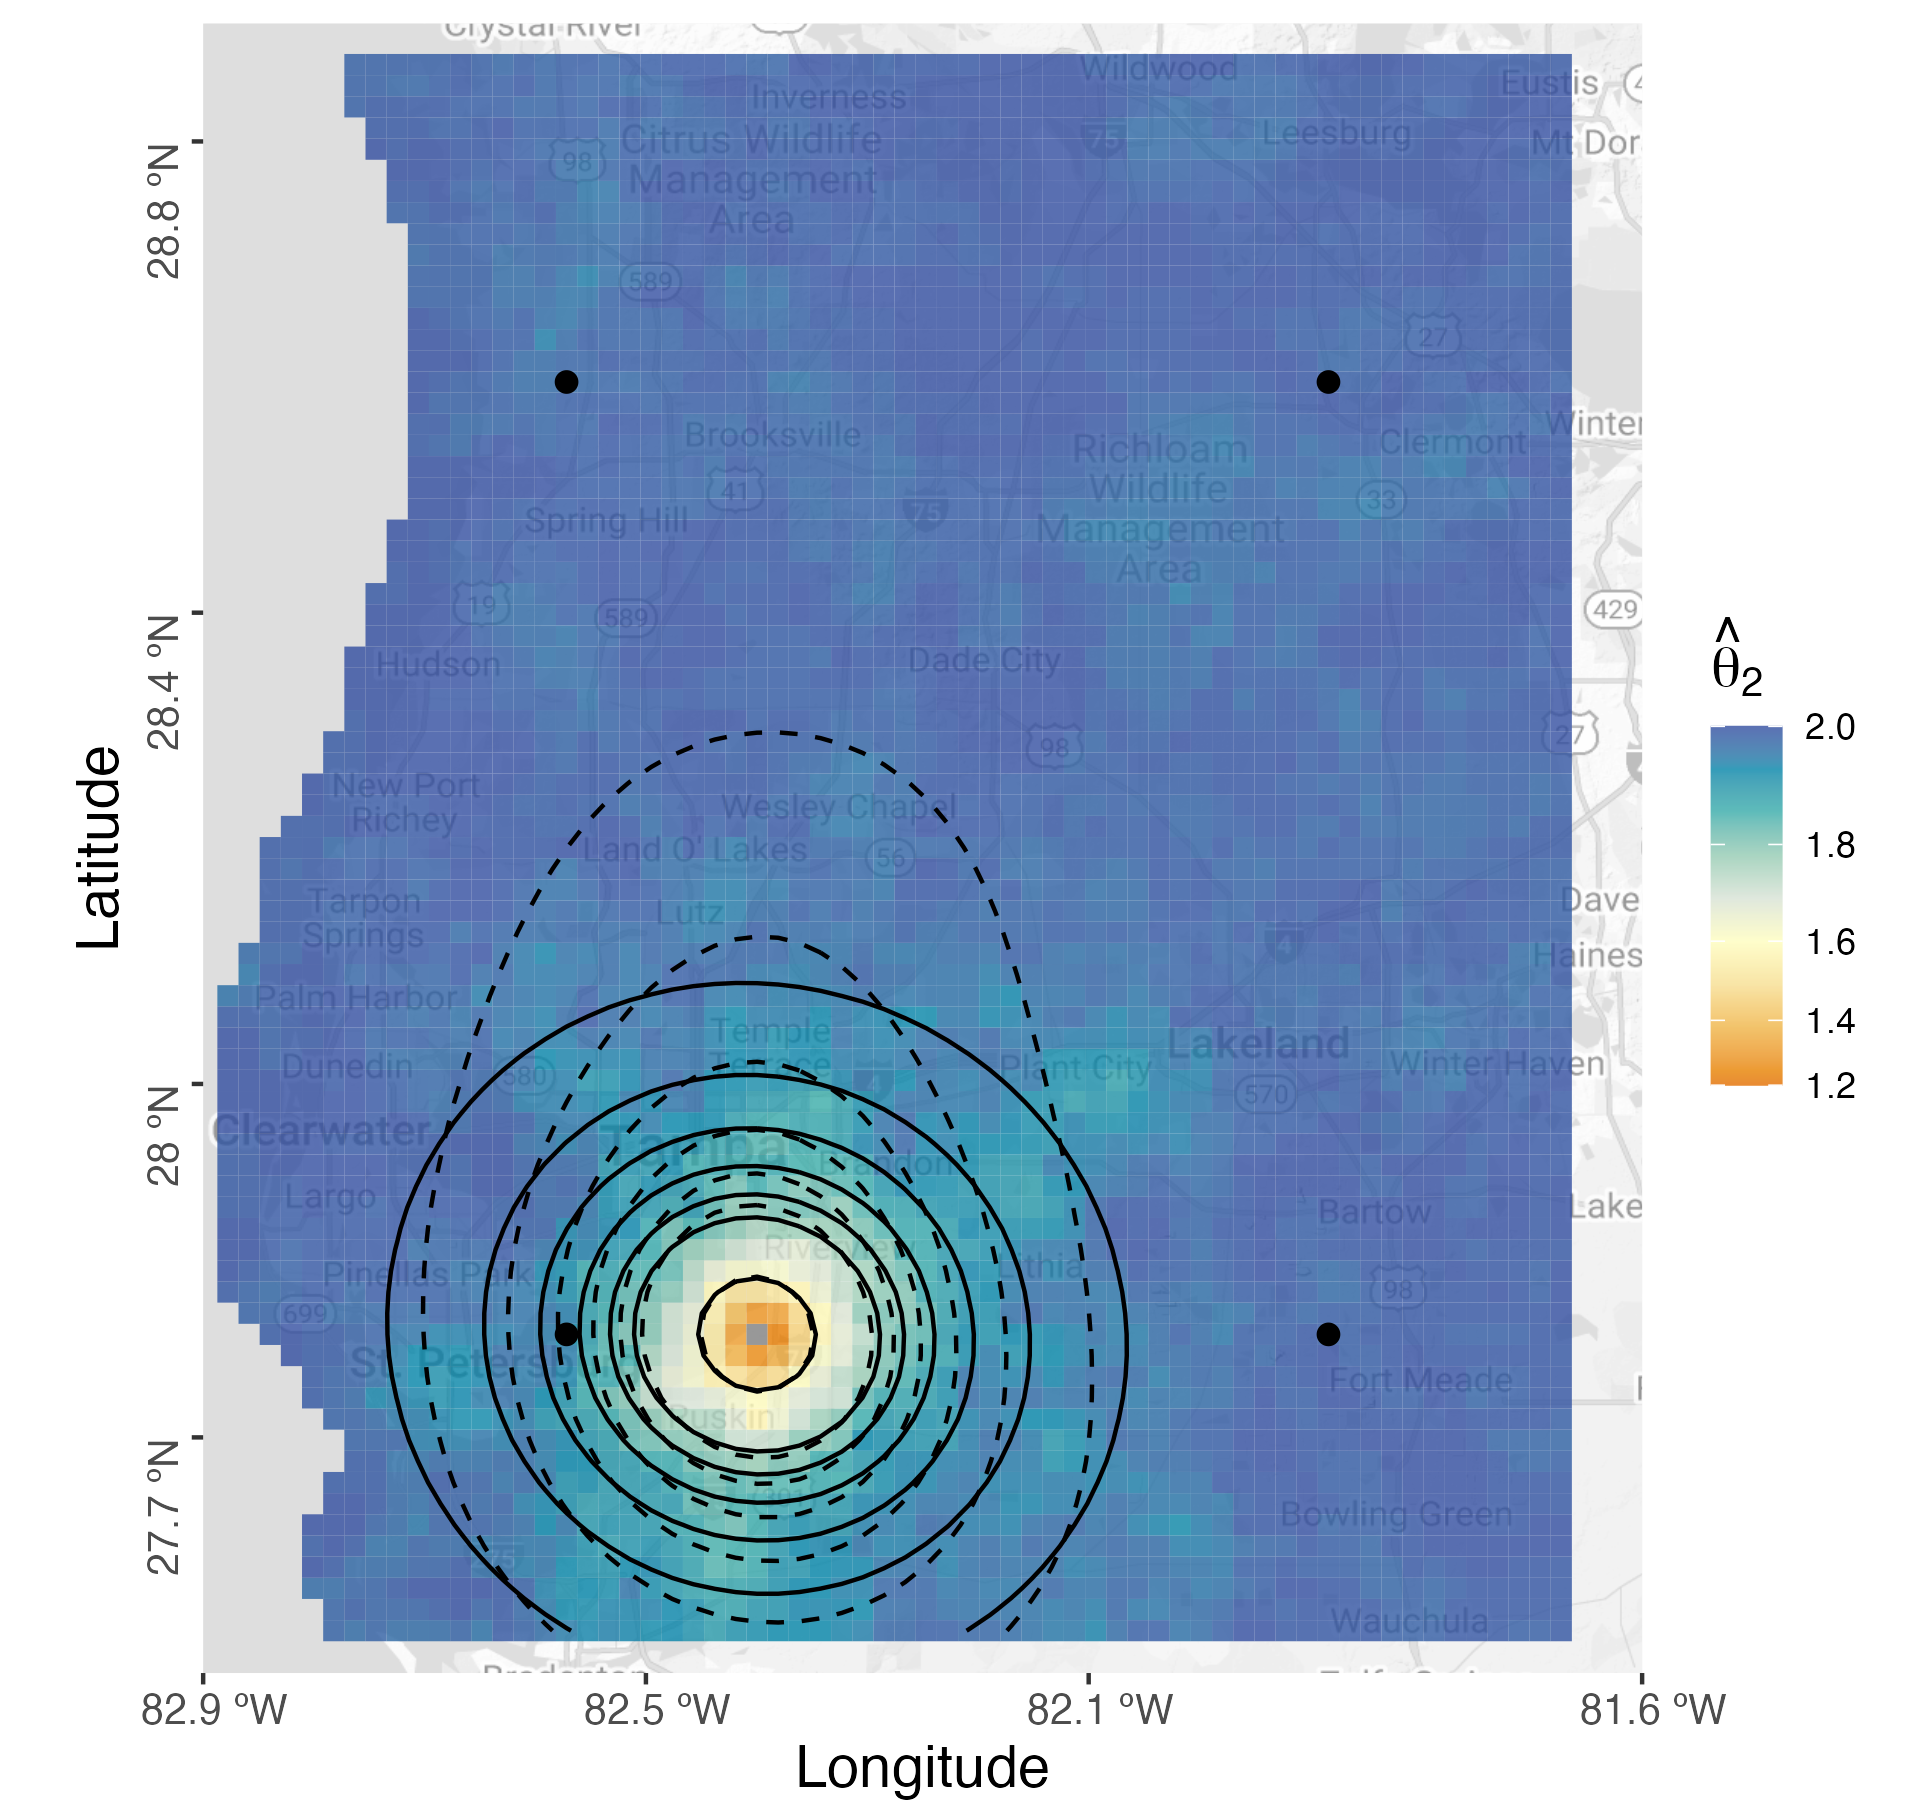
\includegraphics[width=1\textwidth]{florida/florida_extcoef2_1_008.png}
    \end{subfigure}%
    \begin{subfigure}{0.45\textwidth}
        \centering
        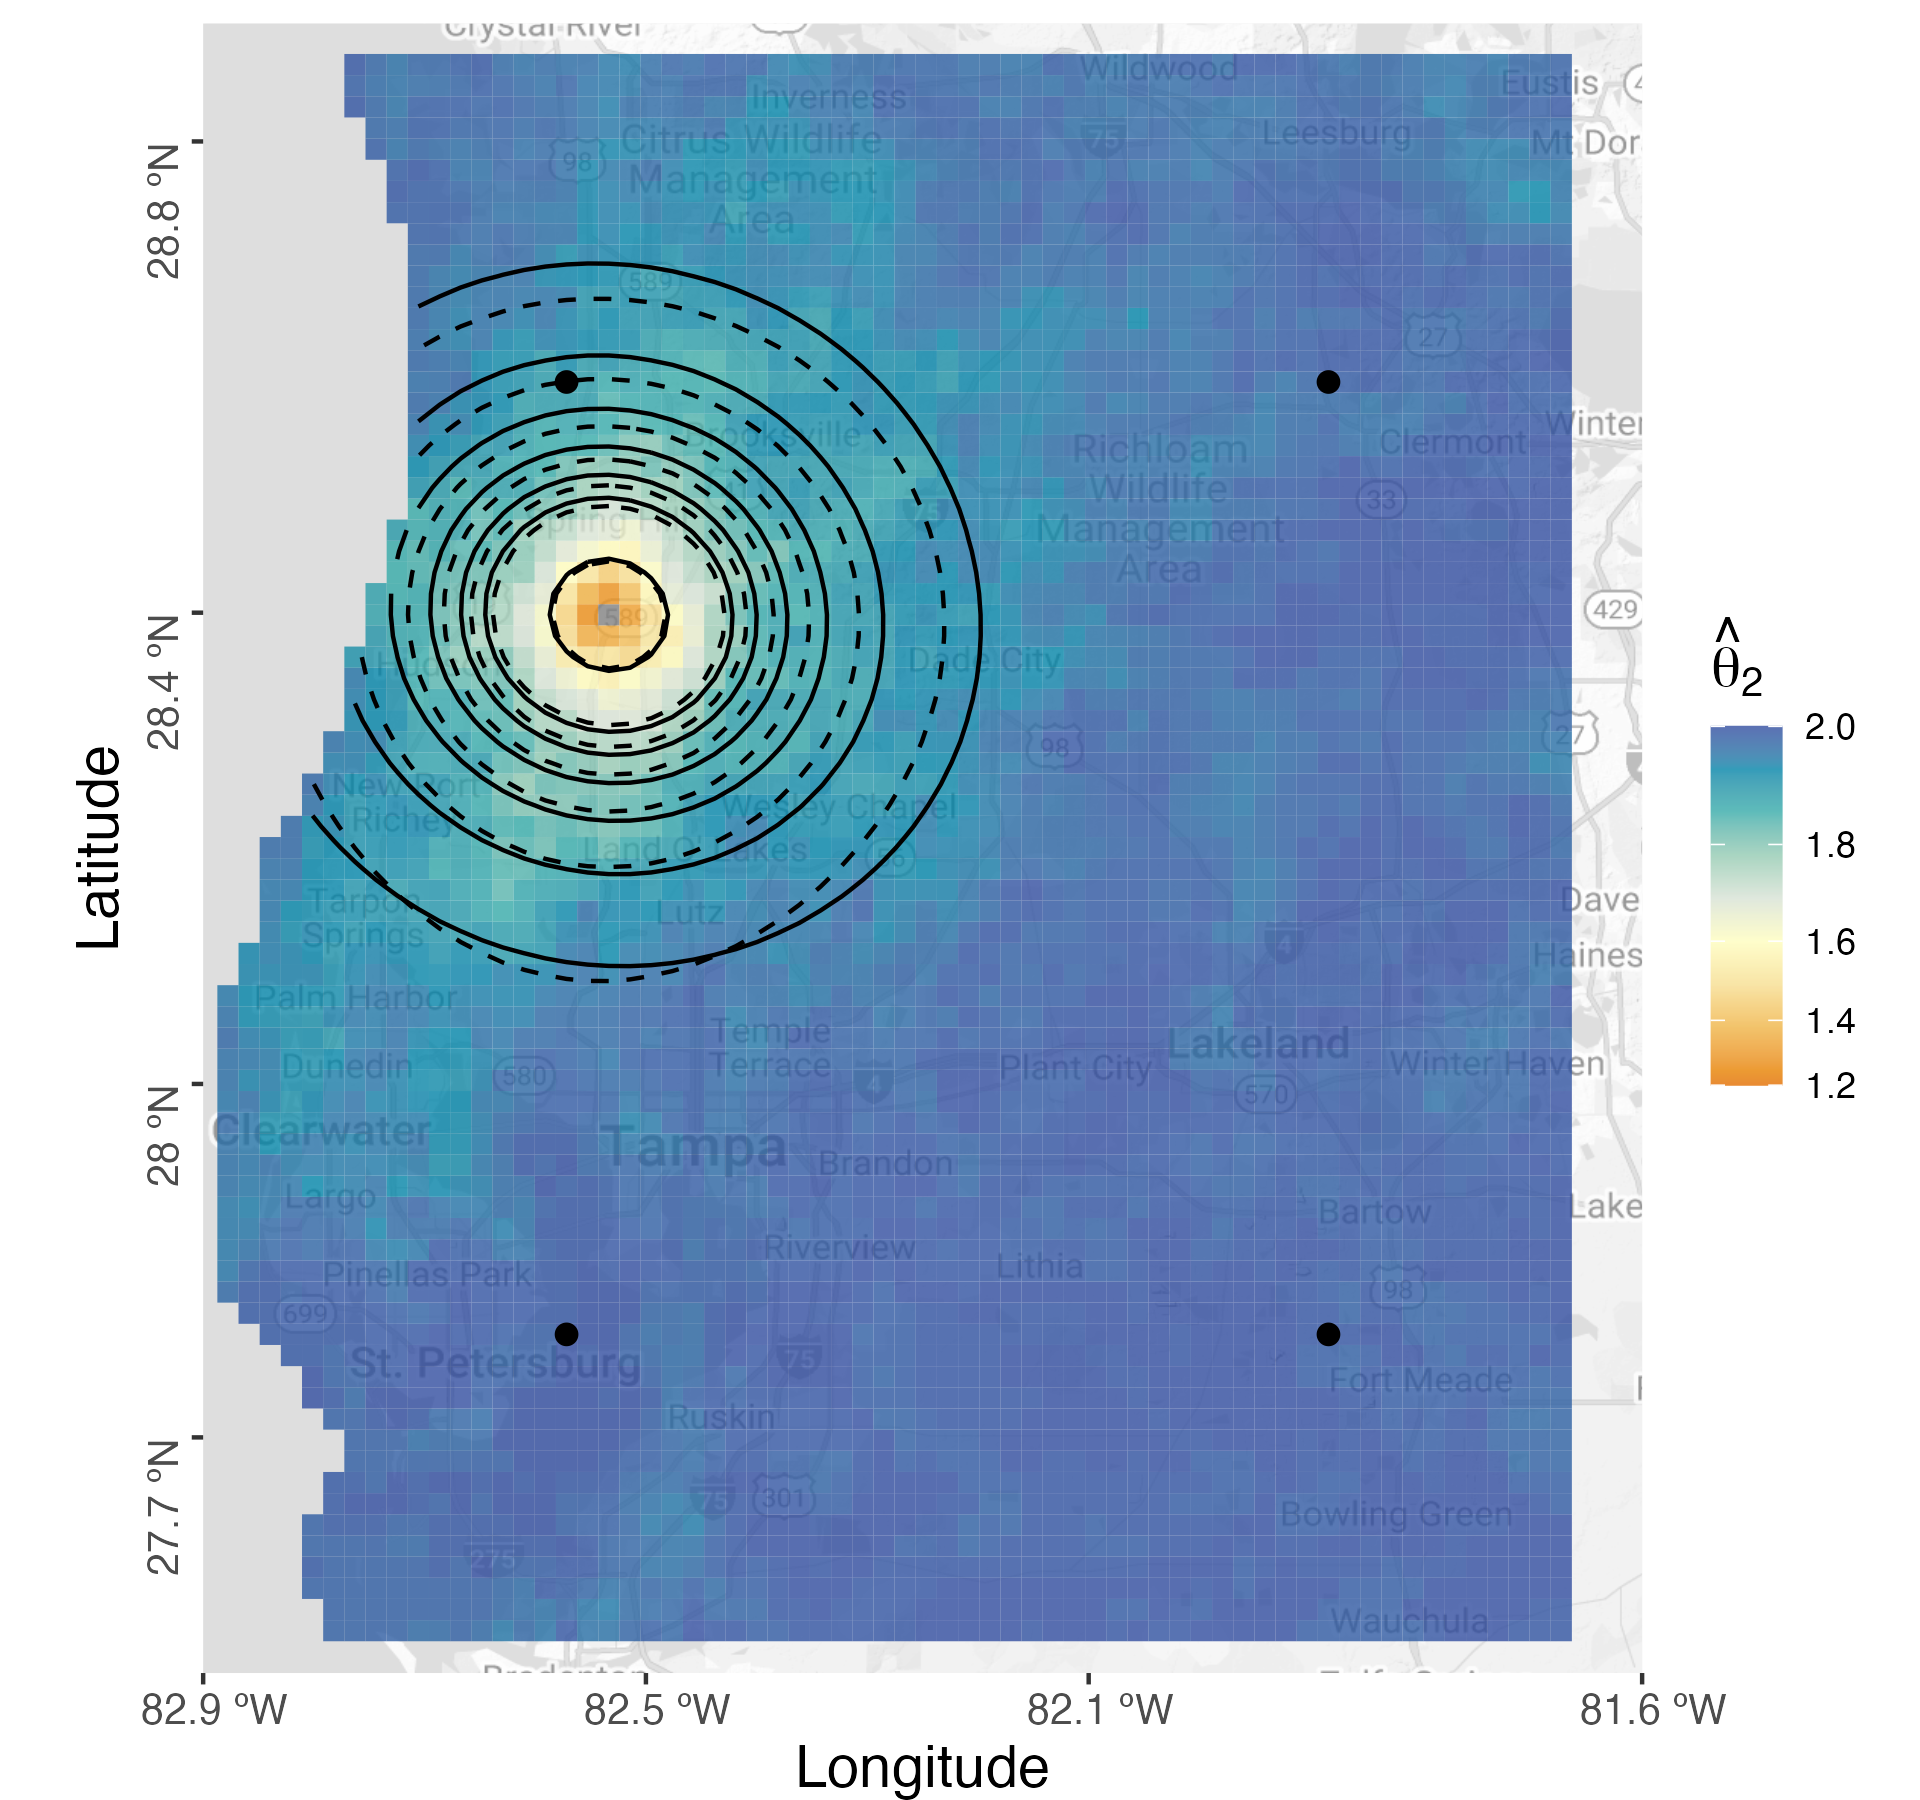
\includegraphics[width=1\textwidth]{florida/florida_extcoef2_1_038.png}
    \end{subfigure}
    % \begin{subfigure}{0.45\textwidth}
    %     \centering
    %     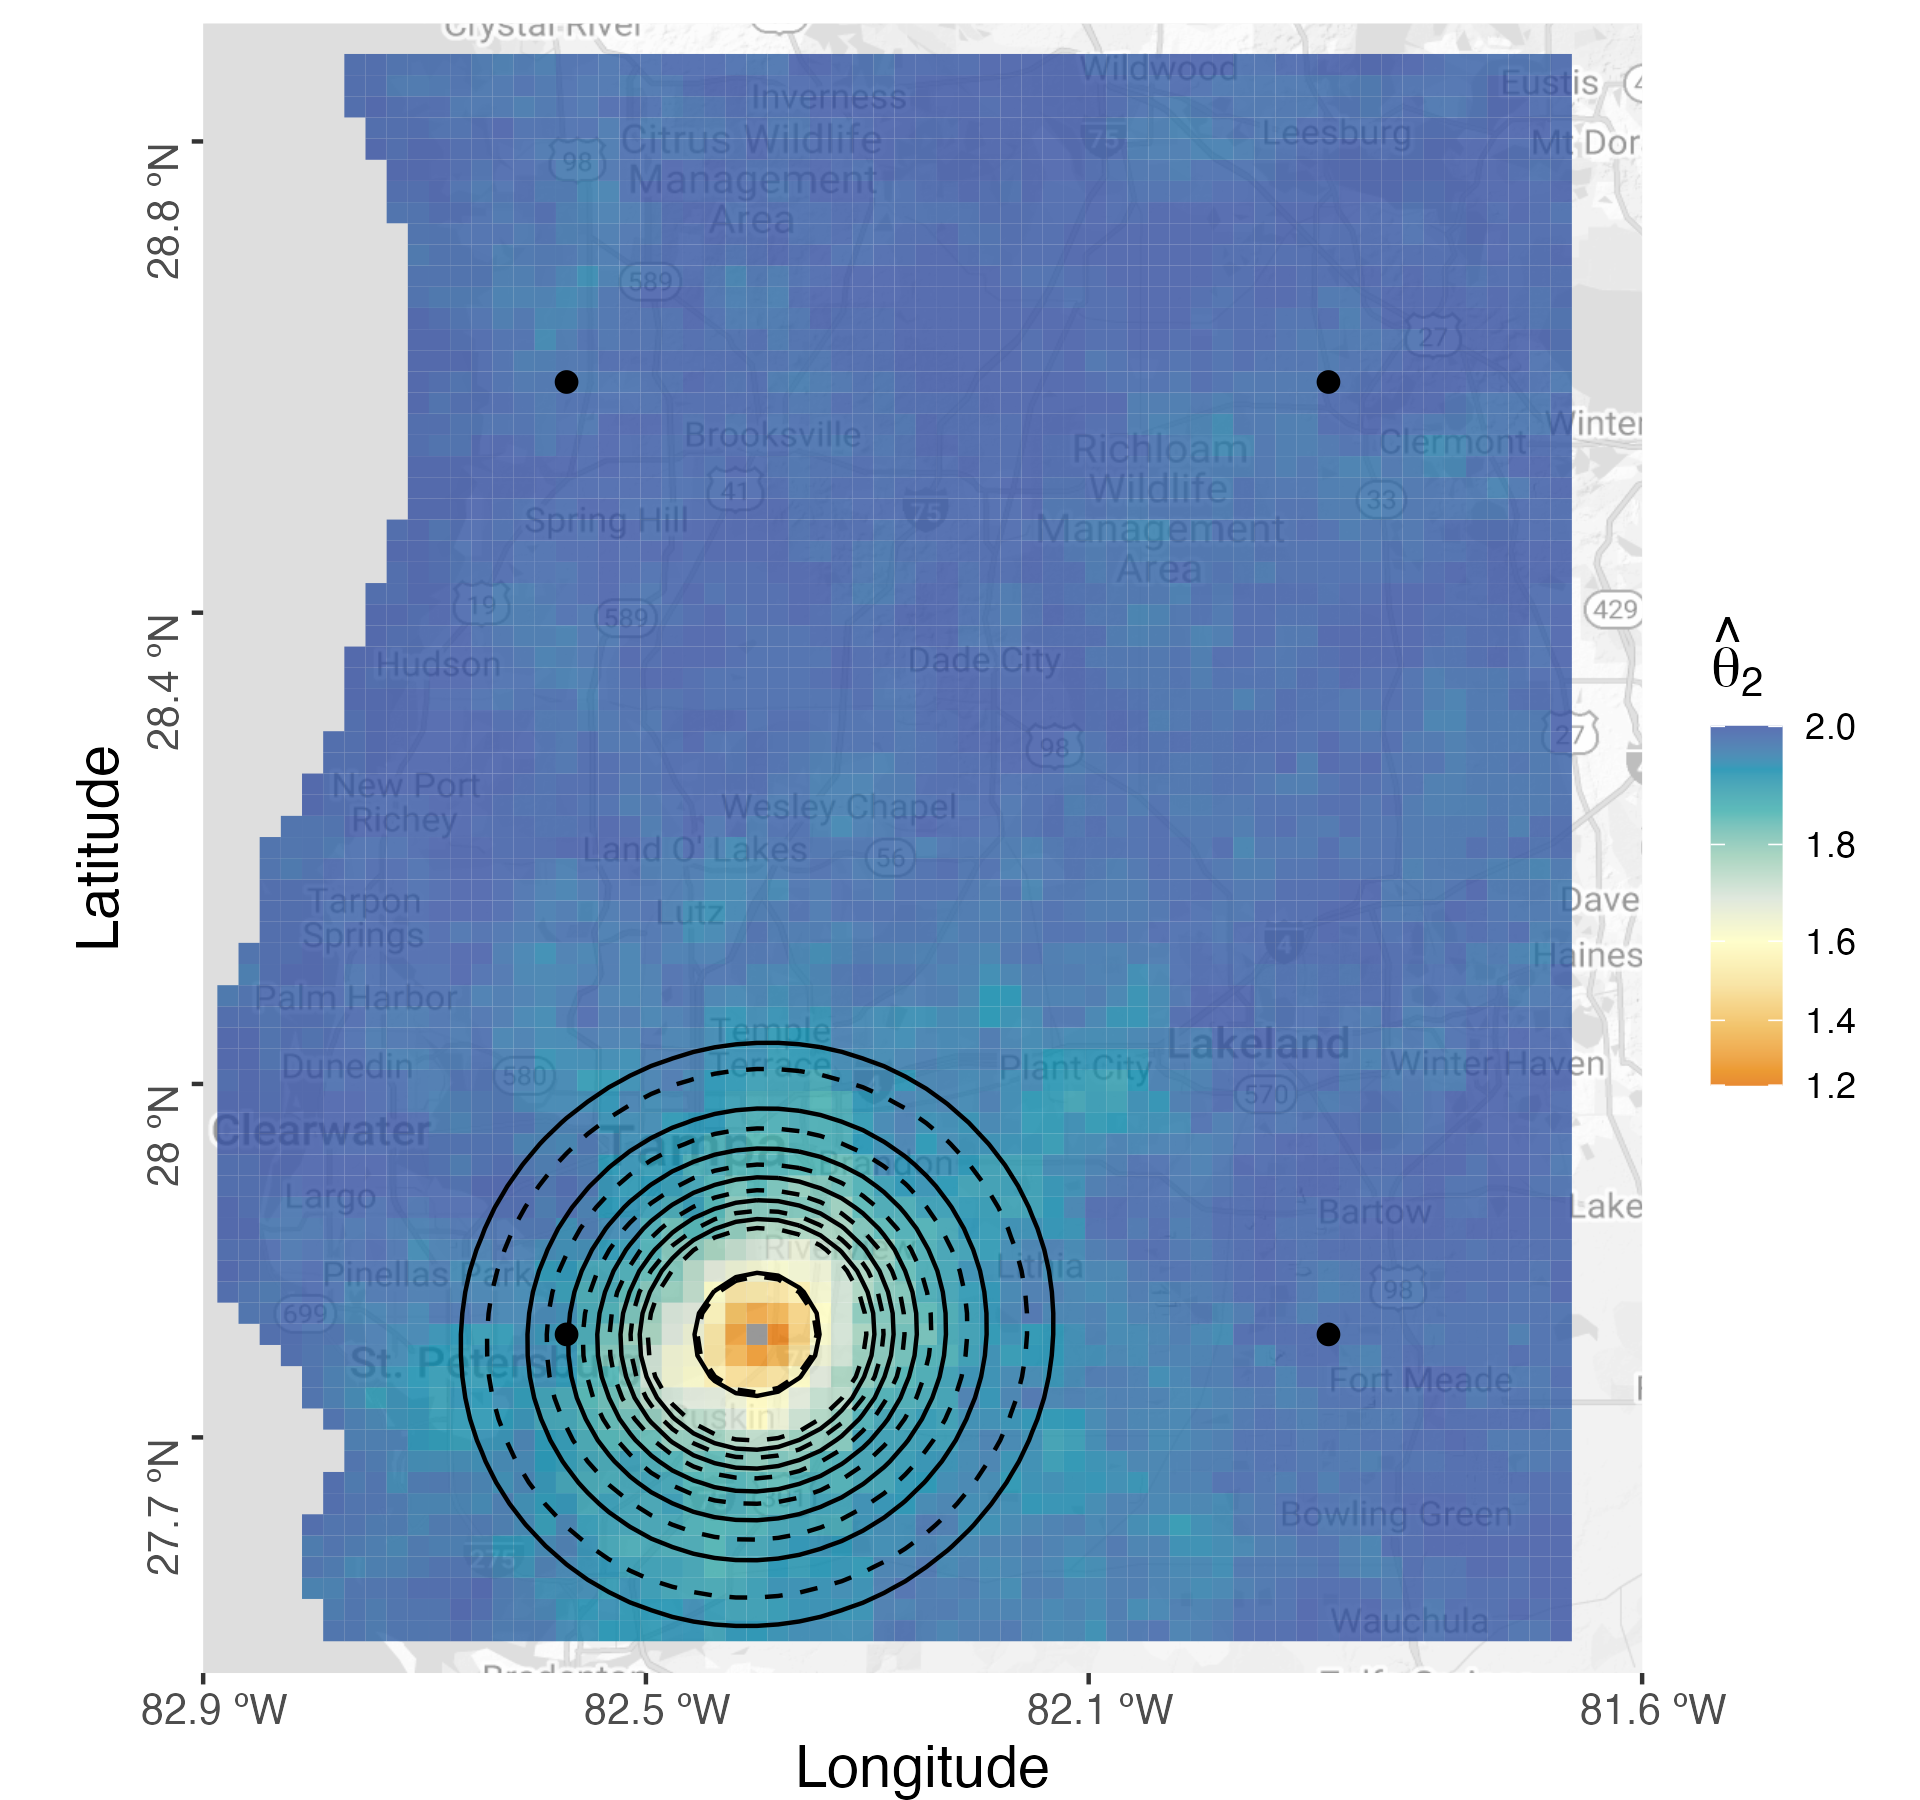
\includegraphics[width=1\textwidth]{florida/florida_extcoef2_2_008.png}
    % \end{subfigure}
    % \begin{subfigure}{0.45\textwidth}
    %     \centering
    %     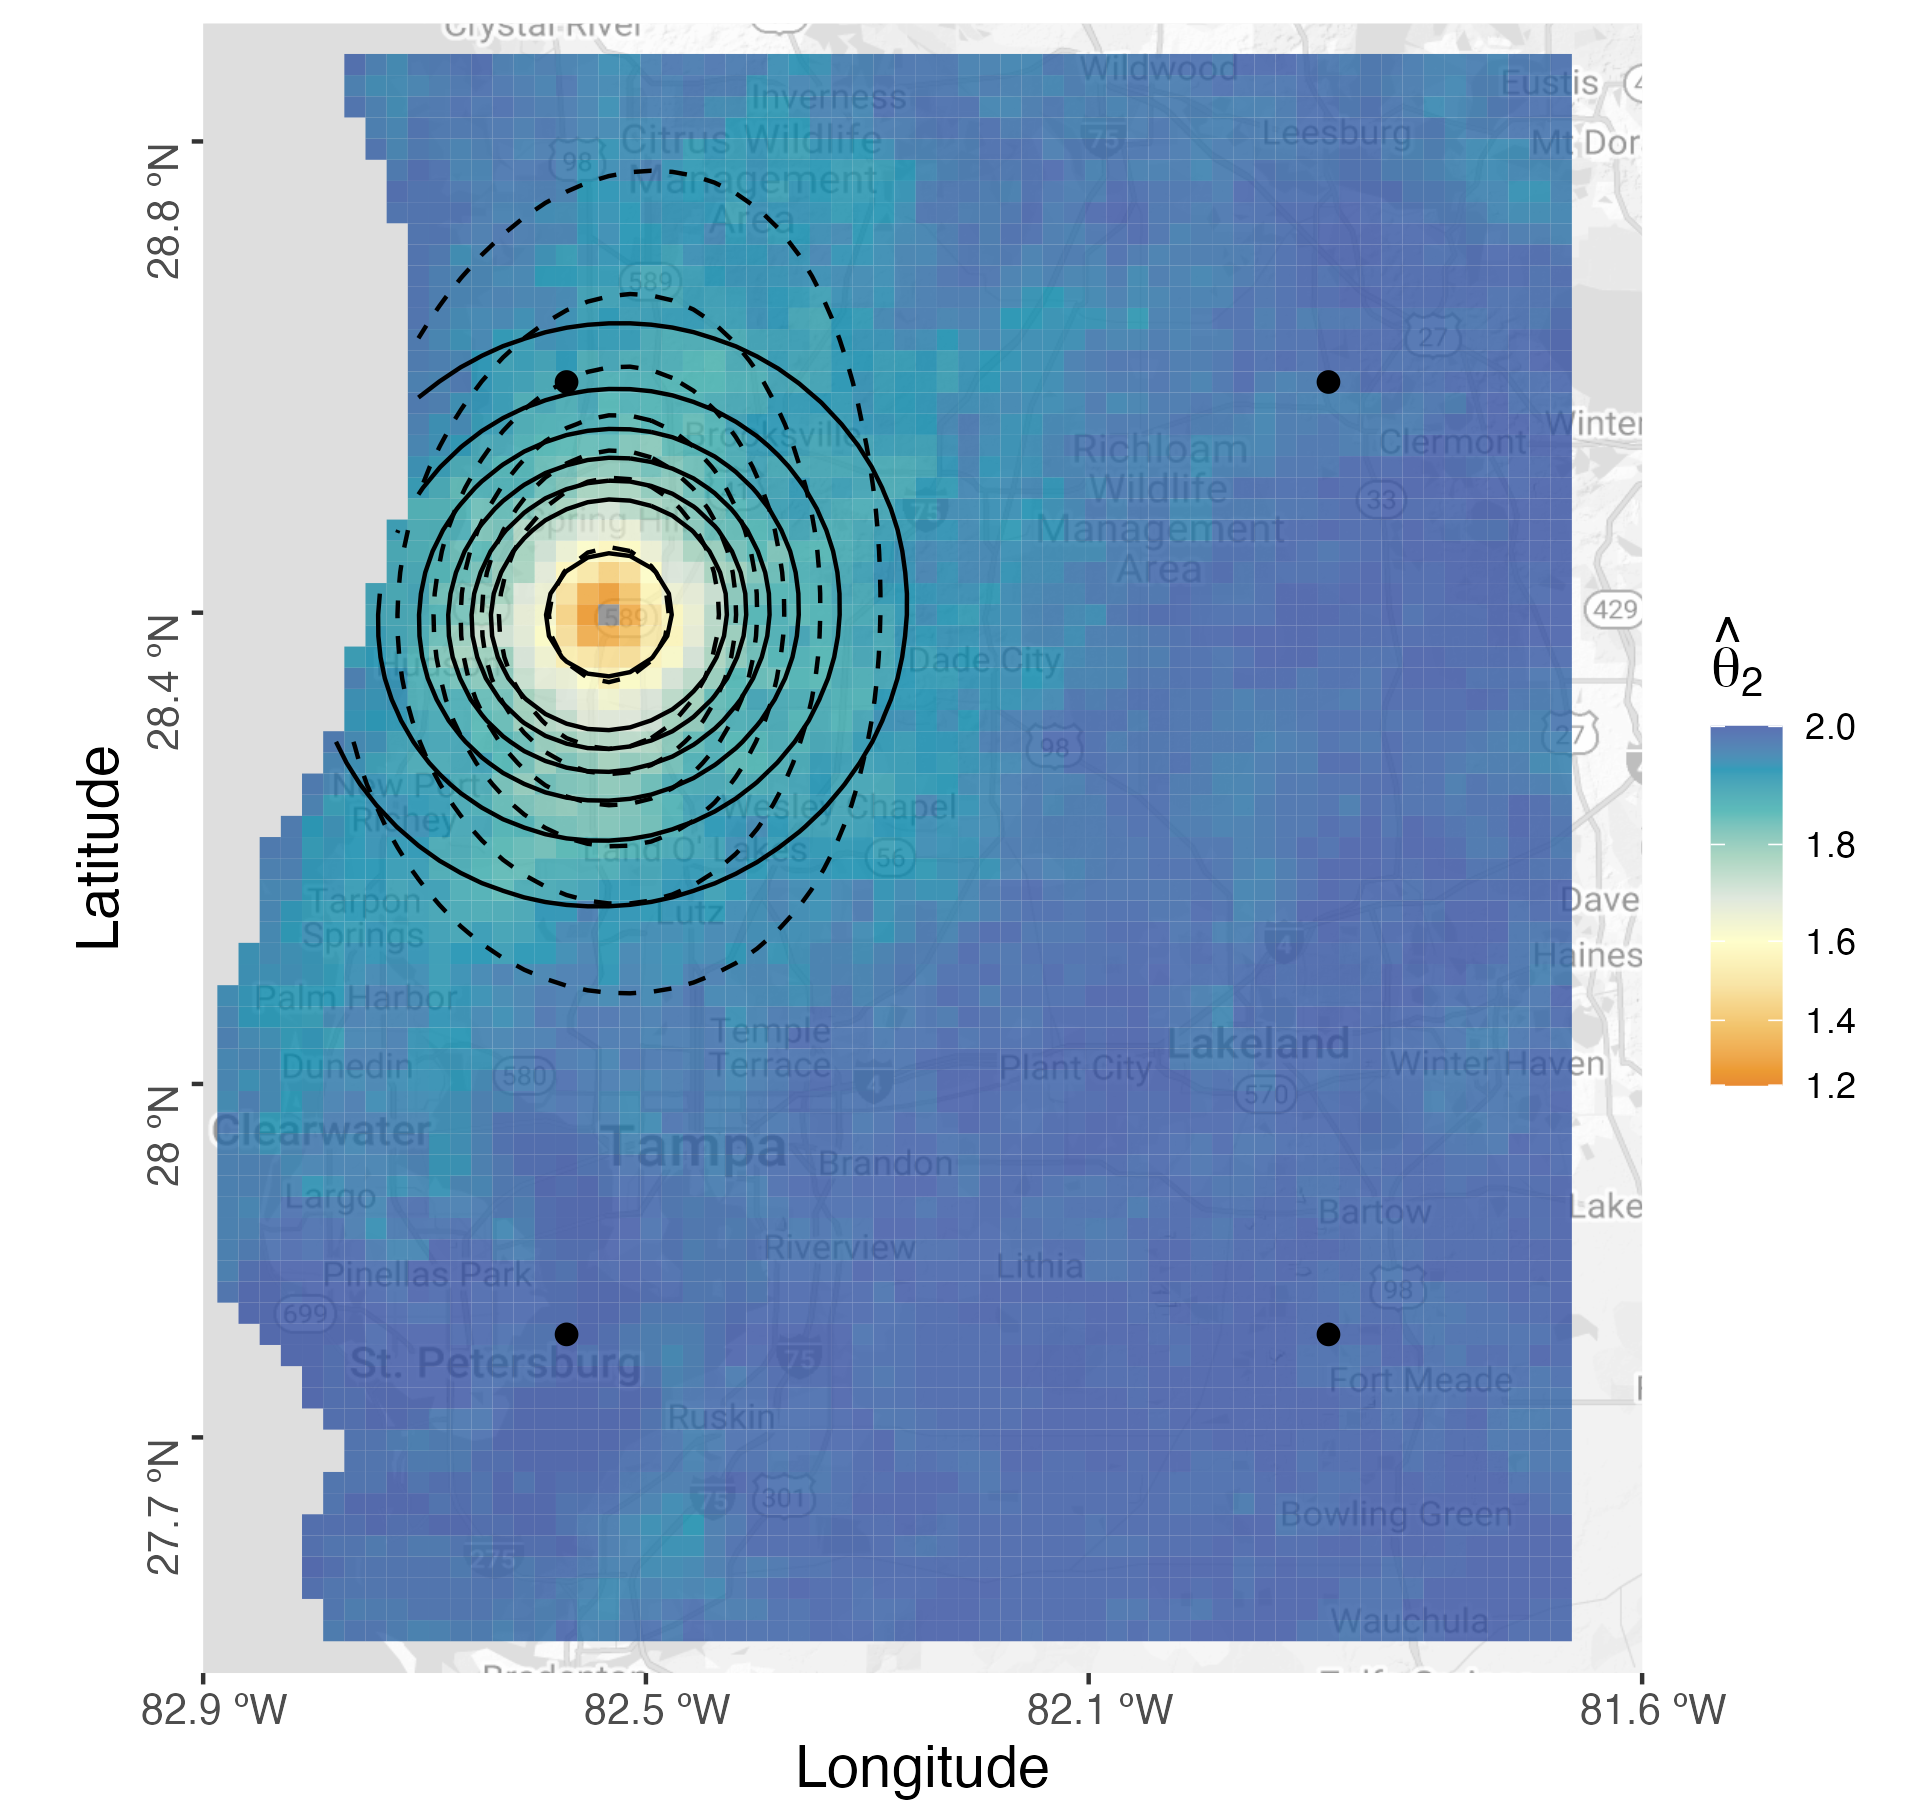
\includegraphics[width=1\textwidth]{florida/florida_extcoef2_2_038.png}
    % \end{subfigure}
    \caption{\small Maps of bivariate empirical extremal coefficients (shading) with respect to two different reference points (columns), and contours of the extremal coefficient of the fitted sBR (dashed line) and BR (solid line) $r$-Pareto models on the Florida rainfall data. 
    % Top and bottom rows use the $L_1$ and $L_\infty$ norm risk functional, respectively. Black dots denote the kernel centres used in the sBR model.
    %for 8 levels (1.2,1.5,1.7,1.75,1.8,1.85,1.9, and 1.95).
    }
    \label{fig:extcoef_application_florida}
\end{figure}


%%%%%%%%%%%%%%%%%%%%%%%%%%%%%%%%%%%%%%%
%%%%%%%%%%%%%%%%%%%%%%%%%%%%%%%%%%%%%%%
\subsection{Analysis of sea surface temperature over the Red Sea}
%%%%%%%%%%%%%%%%%%%%%%%%%%%%%%%%%%%%%%%
%%%%%%%%%%%%%%%%%%%%%%%%%%%%%%%%%%%%%%%

We analyse the spatial dependence structure of the sea surface temperature (in $^\circ \textrm{C}$) over the Red Sea. The data comprise $31$ annual maxima recorded between $1985$ and $2015$ at $D=1,043$ gridded locations. An exploratory analysis by \citet{Hazra.Huser:2021} demonstrated the necessity for a model that captures asymptotic dependence as well non-stationarity. \PZ{Though the study area might be too large to justify a max-stable model over the whole region, as a demonstration of our model, we still follow \cite{Huser.Zhong:2023} to fit a max-stable model and the annual maxima are marginally standardized to unit Fr\'{e}chet scale.} The BR and sBR max-stable process models are fitted using the spectral likelihood with threshold $u=10\times D$, where $10$ is approximately the $90\%$ quantile of the unit Fr\'echet distribution, leaving $9$ observations for model fitting. The spline representation of $\bm\eta$ 
%introduced in 
%(Section~\ref{ssec:flex_dep})
%is also chosen here with
uses $5$ kernel centres 
%selected 
%in the middle of the Red Sea, 
along the Red Sea's North-South axis 
(see black dots in Figure~\ref{fig:extcoef_application_redsea}). 
and as with
%Similarly to 
the previous analysis, no background noise is added. 
% since only $\bm\xi$ needs to be estimated (instead of $\bm\eta$) and so the identifiability of $b_1,\ldots,b_5$
% %$b_i,i=1,\dots,5$ 
% is not a concern. 
%

We contrast model fitting with the spectral likelihood, composite likelihood and Vecchia approximations.
%
The latter was proposed by \cite{Huser.Zhong:2023} for fitting max-stable process models, who demonstrated that it could outperform composite likelihoods when using the Brown-Resnick model with fixed smoothness parameter $\vartheta$. We implement this approach with the anisotropic semi-variogram \eqref{eq:semivar} and directly estimating $\vartheta$.
%
The composite likelihood uses all pairs of first-order (immediate N, S, E, W) neighbours on the grid, yielding $2,046$ pairs. 
%
The parameter estimation results are shown in Table~\ref{tab:parameter_estimates_RedSea}, with only spectral likelihoods being used for the sBR model.

%-------
%\textcolor{red}{\cite{Huser.Zhong:2023} 
%proposed
%%define an 
%inference 
%%methodology 
%for max-stable processes 
%using
%%based on 
%Vecchia approximations which was shown to outperform composite likelihoods when applied to the Brown-Resnick model with fixed smoothness parameter $\vartheta$.
%%  to avoid difficulties in the joint estimation of the range and smoothness parameters
%% In particular, for the dataset under consideration, fixing $\vartheta=1$ proves to be a better choice than $0.5$ or $1.5$.
%% , and so did the pairwise over triplewise composite likelihood. 
%Motivated by the physical properties of the Red Sea and supported by the model fits, anisotropy was introduced in the (semi)-variogram.
%%in a similar way to the previous real data example. 
%%
%Overall, \cite{Huser.Zhong:2023} concluded that the best results are obtained when fixing $\vartheta=1$ and using a Vecchia approximation with $4$ conditioning sites. This procedure is re-ran with the anisotropic semi-variogram described in \eqref{eq:semivar} and letting parameter $\vartheta$ free. Estimates are obtained in $1.41$ hours and reported in Table~\ref{tab:parameter_estimates_RedSea} (model $\textrm{BR}^v$) and in agreement with those observed by \citet{Huser.Zhong:2023}. 
%% with parameter estimates reported to be $\hat{\lambda}=113.9, \hat{\theta} = 0.40$ and $\hat{a}=0.73$ where $a$ is equivalent to $m^2$ in \eqref{eq:aniso_mat} \textcolor{red}{(Peng to confirm)}, and obtained in $5,335$ seconds. 
%%
%For the composite likelihood, the best reported results consider pairs rather than triples and binary weights with a cut-off distance restricting to first-order neighbours, yielding $2,046$ pairs. This approach takes $0.93$ hours  which is faster than the Vecchia approximation approach but \cite{Huser.Zhong:2023} note that for the same likelihood complexity, the Vecchia approximation is much faster and produces better results. 
%}
%-----

\begin{table}[tbh]
    \centering
    \scalebox{0.85}{
        \begin{tabular}{lcccccccccccc}
            \hline
           Model & $\hat\lambda$ & $\hat\vartheta$ & $\hat\zeta$ & $\hat m$ & $\hat b_1$ & $\hat b_2$ & $\hat b_3$ & $\hat b_4$ & $\hat b_5$ & \textrm{Time (hrs)} & \textrm{AIC}\\ 
            \hline                
            $\textrm{BR}^c$ & 58.61 & 1.35 & -0.54 & 0.76 & - & - & - & - & - & 0.93 & -\\ 
              & (14.79) & (0.18) & (0.05) & (0.04) & - & - & - & - & - \\
            $\textrm{BR}^v$ & 108.91 & 1.16 & 0.79 & 1.21 & - & - & - & - & - & 1.41 & -\\ 
              & (12.20) & (0.09) & (0.10) & (0.06) & - & - & - & - & - \\
            $\textrm{BR}$ & 64.78 & 1.16 & 0.79 & 1.14 & - & - & - & - & - & 0.17 & 16782.41 \\ %1871.82\\ 
              & (7.06) & (0.10) & (0.16) & (0.05) & - & - & - & - & - \\  
            sBR & 51.36 & 1.33 & 0.79 & 1.12 & -13.49 & -8.31 & 2.05 & 12.85 & 15.07 & 0.65 & 16445.17 \\ %1843.46 \\ 
              & (4.75) & (0.09) & (0.28) & (0.07) & (15.48) & (6.76) & (9.32) & (7.58) & (11.47) & \\ 
            \hline
        \end{tabular}
    }
    \caption{\small Parameter estimates (with jackknife estimates of the standard errors) for the Brown-Resnick (BR) and skewed Brown-Resnick (sBR) max-stable process models on the Red Sea data. Model name with superscript $v$ or $c$ denotes inference using  Vecchia or composite likelihood approximations, respectively. No superscript indicates use of the spectral likelihood.}
    \label{tab:parameter_estimates_RedSea}
\end{table}

Focusing on the Brown-Resnick parameter estimates, Table~\ref{tab:parameter_estimates_RedSea} indicates broadly comparable statistical efficiency 
% of the spectral likelihood (i.e., model $\textrm{BR}$) is comparable with the composite likelihood and Vecchia approximation 
across all
methods and Vecchia estimates in agreement with those observed by \citet{Huser.Zhong:2023}. By displaying the fitted extremal coefficients, Figure~6 of the Supplementary Material illustrates that even though the pairwise likelihood estimates ($\textrm{BR}^c$) reported in Table~\ref{tab:parameter_estimates_RedSea} seem slightly different to those from the other methods, they lead to a similar dependence structure. In terms of computational efficiency the spectral likelihood is respectively $\sim 4.5$ and $\sim 7.3$ times 
% $447\%$ and $729\%$ 
faster than the composite and Vecchia approaches. 
%
%(\cite{Huser.Zhong:2023} note that for the same likelihood complexity, the Vecchia approximation can be faster and better performing than the composite likelihood.)
%
% The spectral likelihood approach does not require fixing $\vartheta$ and the Brown-Resnick estimates are \textcolor{red}{$\left( \hat{\lambda}, \hat{\vartheta}\right) = \left(69.04, 1.19\right)$} with jackknife standard deviations \textcolor{red}{$(4.85,0.04)$}, and were obtained in \textcolor{red}{$3.27$} minutes on a single core. 
% 
% Comparatively, the method of \cite{Huser.Zhong:2023} which relies on the pairwise composite likelihood with less than $2,000$ pairs and fixed smoothness parameter $\vartheta$, takes $31$ seconds using 32 cores while fixing the smoothness parameter .
%
Fitting the skewed Brown-Resnick model with the spectral likelihood yields a smaller estimate of $\lambda$ and  a larger estimate of $\vartheta$ than for the Brown-Resnick. This is somewhat expected as the fitted skewed Brown-Resnick model better accounts for the dependence strength and structure than the Brown-Resnick model. 
%Similarly to the rainfall analysis, the large standard error estimates for the $b_1, \ldots, b_5$ parameters cannot be used to conclude that these parameters aren't useful. 
%On top of the identifiability issues that might be present (but not detrimental to the insights), we recall that only 9 observations of the preocess are used for fitting a 9 parameter model. 
Even with the additional parameters, the AIC favours the skewed Brown-Resnick model over the regular Brown-Resnick model, indicating improved modelling of spatial dependence. 
We also note that fitting the sBR model using the spectral likelihood is faster than fitting the BR using the Vecchia or composite likelihood approaches.
%using existing approaches.

% \textcolor{red}{[NEED TO RE-RUN MODELS WITH ANISOTROPIC SEMI-VARIROGRAM]}
% The above estimates indicate that the parameters are identifiable, due to the large number of locations and kernel spline used.
% % 
% For the Brown-Resnick model, the parameter estimation takes $196$ seconds on a single core, yielding $\left( \hat{\lambda}, \hat{\vartheta}\right) = \left(69.04, 1.19\right)$ with jackknife standard deviations $(4.85,0.04)$. In comparison, the method of \cite{Huser.Zhong:2023}, relying on the pairwise composite likelihood with less than 2000 pairs, takes $31$ seconds using 32 cores while fixing the smoothness parameter $\vartheta$. In that context, with fixed $\vartheta$ the spectral likelihood takes $57$ seconds using a single core and produces similar results. The skewed Brown-Resnick estimates are $\left( \hat{\lambda}, \hat{\vartheta}, \hat{b_1}, \hat{b_2},\hat{b_3},\hat{b_4},\hat{b_5}\right) = \left(53.12,1.37,-86.99,29.74,-69.96,4.79, 120.59\right)$, which were obtained in 39.5 minutes using 12 cores.
% %with the three-stage optimisation method. 
% The estimated $\hat\lambda$ is smaller but the estimated $\hat\vartheta$ is larger than the corresponding estimates for the Brown-Resnick model, which is to be expected as the estimated skewed Brown-Resnick model more properly accounts for the dependence strength and structure compared with the Brown-Resnick model. The corresponding estimated standard deviations based on the jackknife are $(2.83,0.05,14.08,1.82,1.66,3.37,1.92)$, suggesting that only one of the estimated slant parameters is insignificant.
% % Finally, since the two models are nested, the Akaike Information Criterion can be used for model selection, confirming a better fit when including skewness in the distribution of the underlying process (AIC=-16458.04 versus -16430.1 for the Brown-Resnick).  

To assess the goodness of fit and visualise the differences in dependence structures from the fitted models, Figure~\ref{fig:extcoef_application_redsea} shows maps of the bivariate extremal coefficient for two reference locations. Both empirical maps  (shading) display some degree of non-stationarity in the dependence structure, in agreement with \citet{Hazra.Huser:2021}, with the contours of the extremal coefficient obtained from the skewed Brown-Resnick model (dashed lines) being able to better capture this phenomena. 
In particular, the skewed Brown-Resnick model
%Together the panels of Figure~\ref{fig:extcoef_application_redsea} give evidence that the extremal coefficient from the proposed model 
is able to simultaneously characterise the differing behaviour observed in the north and south of the Red Sea.
%, whereas previous studies had to restrict the modelling to
% each region separately
% %to one region at a time 
% \citep[e.g.,][]{Simpson.Wadsworth:2020}.


\begin{figure}[ht]
    \centering
    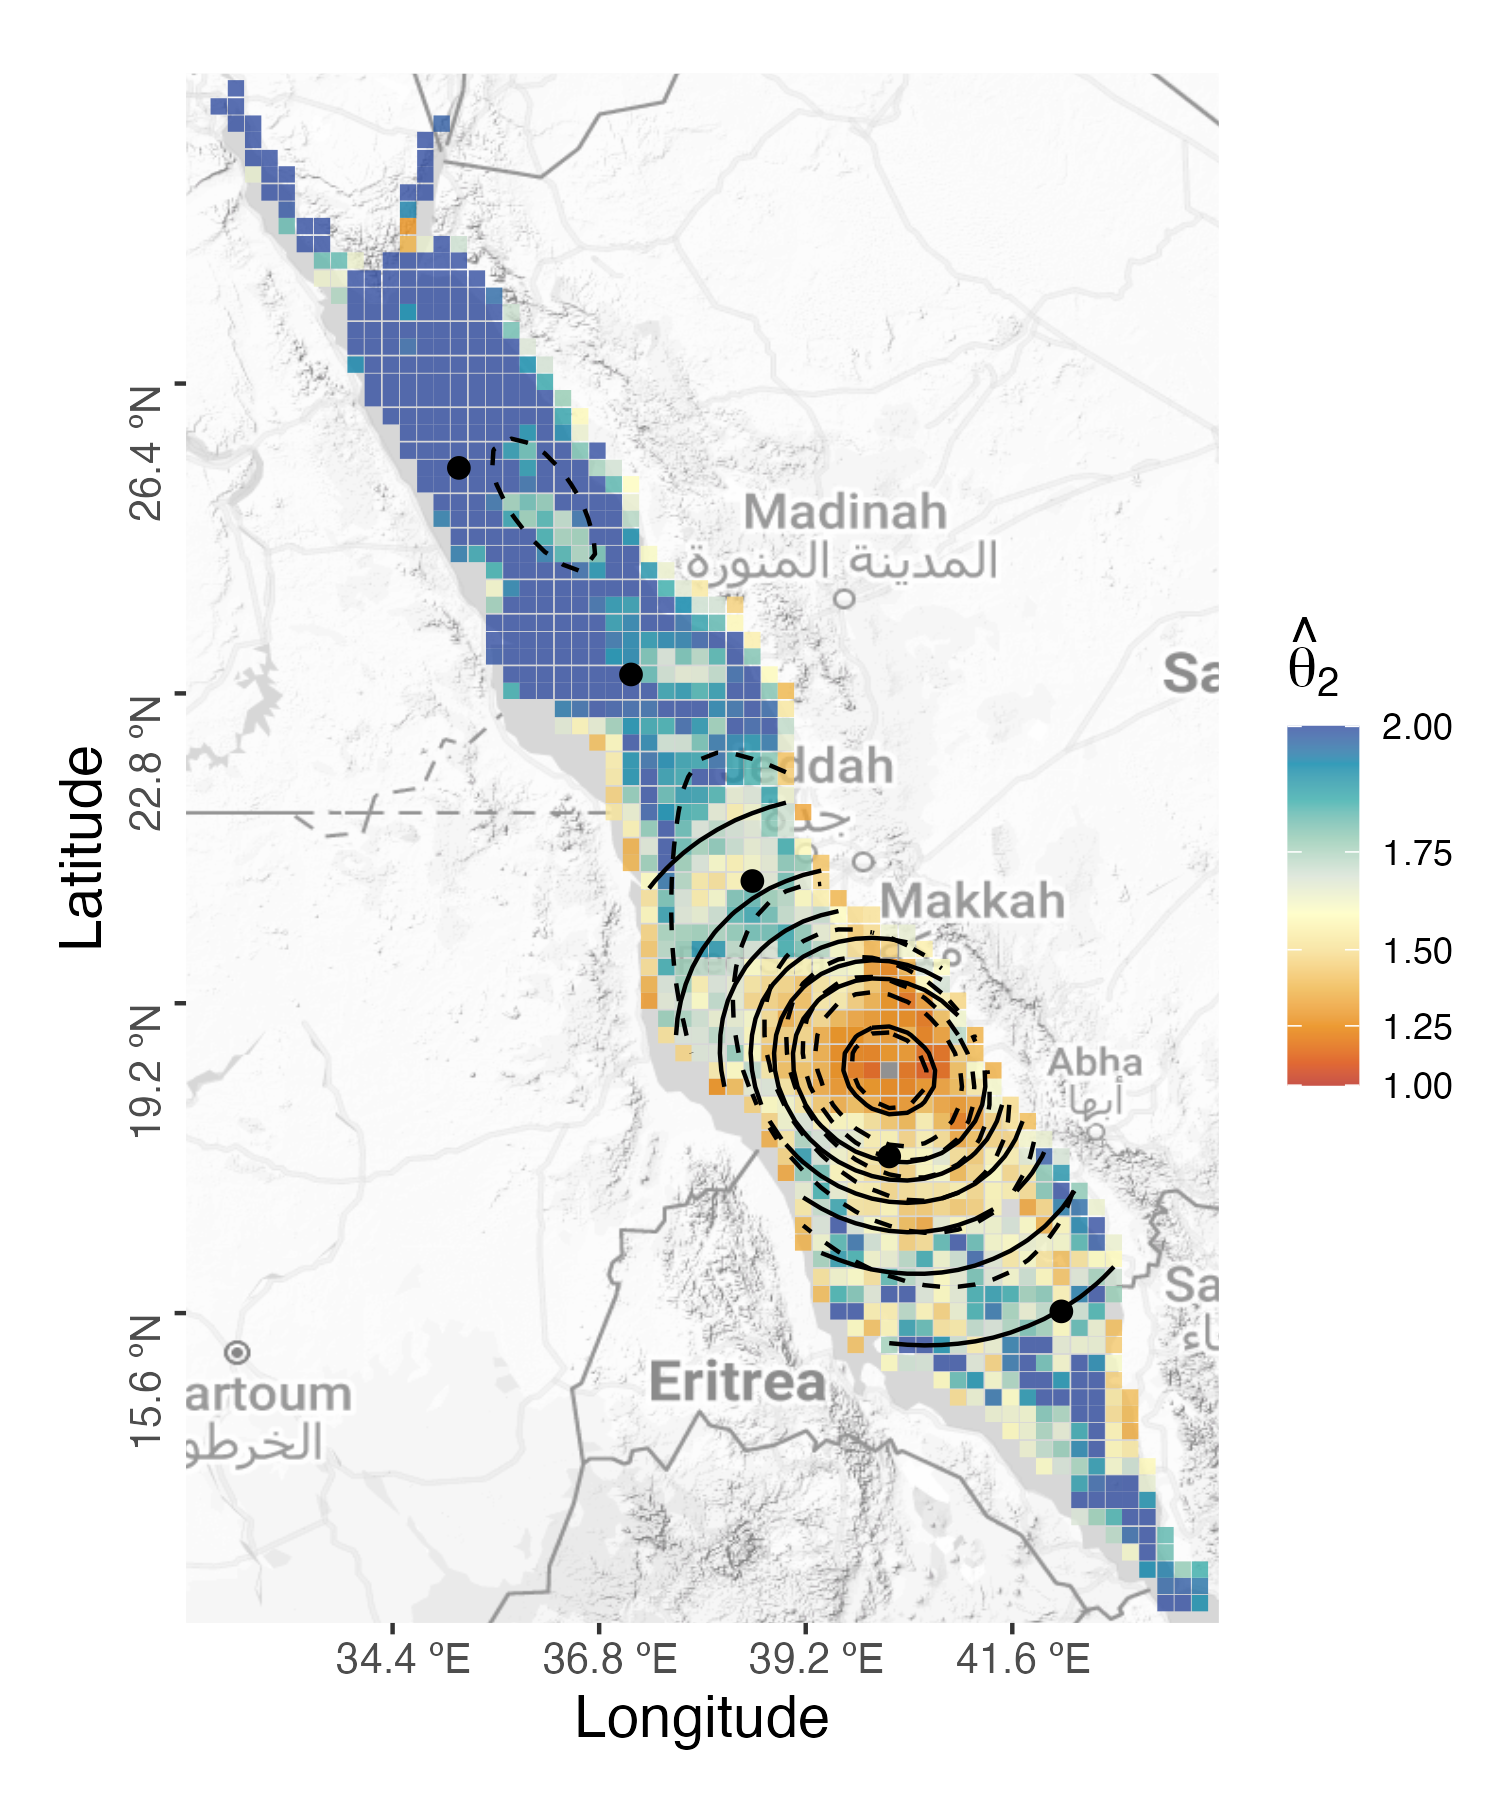
\includegraphics[width=0.49\textwidth]{RedSea2/RedSea_extcoef2_1_035.png}
    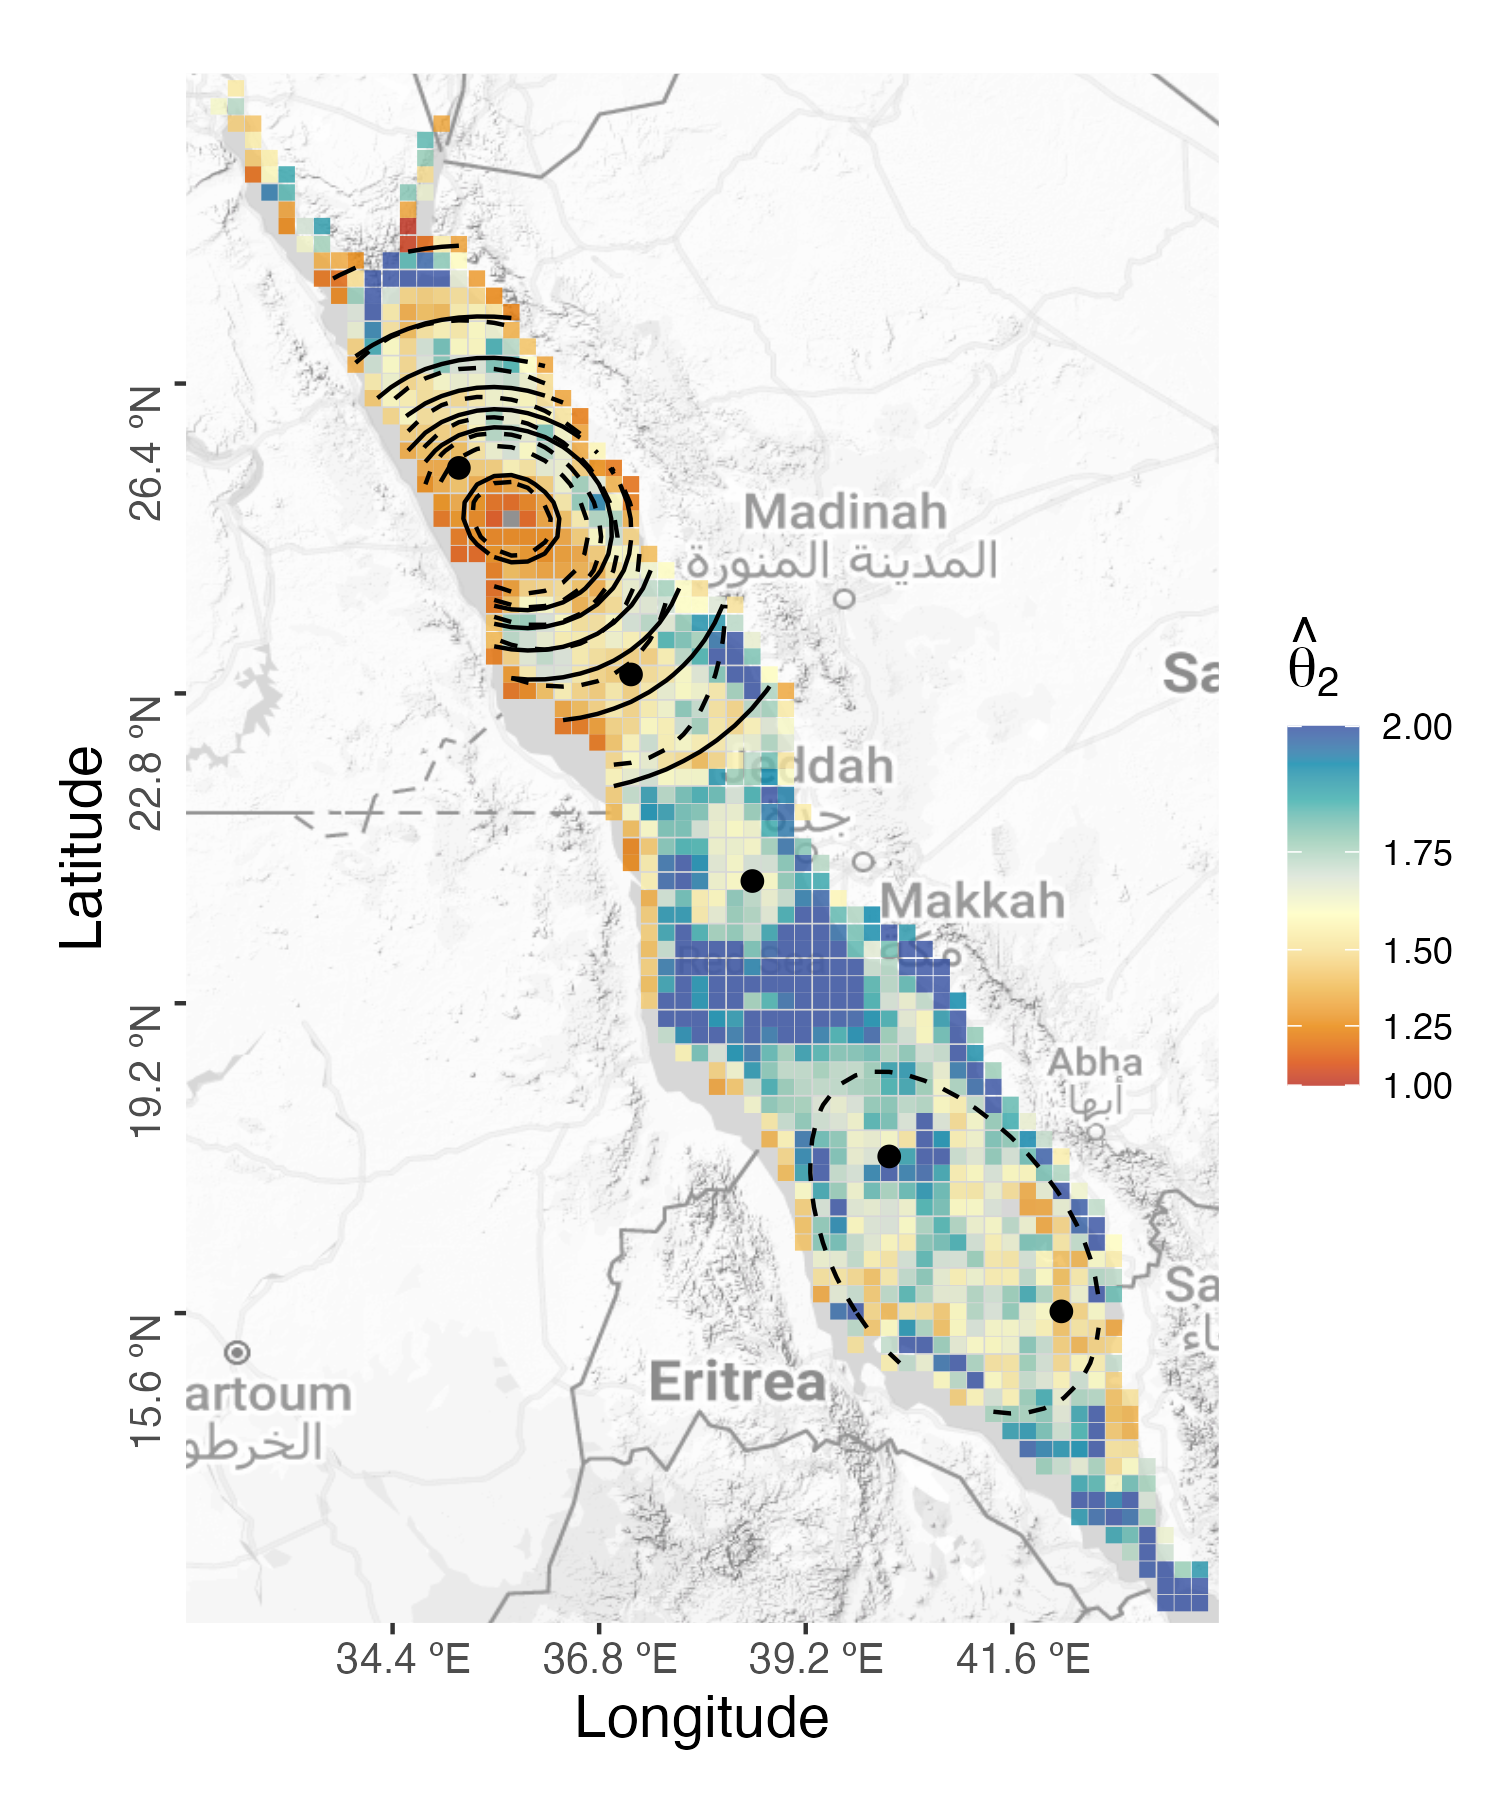
\includegraphics[width=0.49\textwidth]{RedSea2/RedSea_extcoef2_1_082.png}
    \caption{\small Maps of the bivariate empirical extremal coefficient (shading) with respect to two reference locations (left and right panels) with contours curves of the estimated extremal coefficients from the Brown-Resnick (solid) and skewed Brown-Resnick (dashed) models. Black dots indicate the kernel centres used in the skewed Brown-Resnick model.}
    \label{fig:extcoef_application_redsea}
\end{figure}

%%%%%%%%%%%%%%%%%%%%%%%%%%%%%%%%%%%%%%%
%%%%%%%%%%%%%%%%%%%%%%%%%%%%%%%%%%%%%%%
%%%%%%%%%%%%%%%%%%%%%%%%%%%%%%%%%%%%%%%
\section{Discussion}
%%%%%%%%%%%%%%%%%%%%%%%%%%%%%%%%%%%%%%%
%%%%%%%%%%%%%%%%%%%%%%%%%%%%%%%%%%%%%%%
%%%%%%%%%%%%%%%%%%%%%%%%%%%%%%%%%%%%%%%

In this paper, we have established the condition ensuring the intensity function of a max-stable process only places mass on $\Omega^\circ$, the interior of 
% the $D$-dimensional simplex.
its domain.
This condition directly implies that there are no discontinuities in the associated exponent measure, greatly simplifying the evaluation of the finite dimensional density of the corresponding $r$-Pareto process. 
%
As a result, we were able to demonstrate that for models possessing the above property, likelihood-based inference can be successfully implemented via the spectral likelihood \eqref{eq:angular_likelihood_1}. This both opens up viable solutions to the likelihood intractability of max-stable models, and also creates opportunities for the development of new classes of $r$-Pareto models that can better describe real-world processes. Indeed, out of the two primary max-stable models in current use, namely the Brown-Resnick and extremal-$t$, only the former fulfills the continuity condition and is therefore, almost exclusively, the only $r$-Pareto model used in the literature. 

As a first step to address this,
\PZ{we derived two new models: the \emph{skewed Brown-Resnick model} for spatial extremes, which offers greater flexibility than the Brown-Resnick model by allowing for non-stationarity and local anisotropy; and the \emph{truncated extremal-$t$ model} for multivaraite extremes, which mimics the extremal-$t$ while ensuring the 
continuity condition holds. }
Exact simulation algorithms for these new max-stable models can leverage existing simulation techniques, whereas for the associated $r$-Pareto processes we have introduced a more efficient simulation algorithm than the current state-of-the-art. 

% Following the reasoning of the latter, we have demonstrated that the inferential intractability issues for $r$-Pareto models with any risk functional can be bypassed by simply considering the likelihood of a $r$-Pareto models with $L_1$ risk functional.


Using these new models, we have demonstrated
the need for better, more flexible models for
%is illustrated on 
modelling both threshold exceedances and annual maxima data, 
by providing new insights about the non-stationary dependence structure of extreme precipitation and sea surface temperature levels over previous analyses \citep{deFondeville.Davison:2018,Huser.Zhong:2023}. 
The proposed methodology is 
%proven to be 
computationally more efficient than state-of-the-art techniques, such as score matching \citep{deFondeville.Davison:2018} and Vecchia approximation \citep{Huser.Zhong:2023}, 
%allowing to deal with 
thereby enabling the analysis of much higher dimensional data. 

The new models introduced here are one step towards building spatial extreme models that are well-suited for real-world problems.
\PZ{They also open new opportunities in related areas, such as modeling extremes conditioning on a single site, and expanding the class of extremal graphical models with flexible dependence structures}, as currently the only practical models for graphical extremes are constructed from the restrictive Brown-Resnick or H\"usler-Reiss models \citep{Engelke.Hitz:2020,Hentschel.Engelke.Segers:2024,Wan.Zhou:2023}. 


%%%%%%%%%%%%%%%%%%%%%%%%%%%%%%%%%%%%%%%
%%%%%%%%%%%%%%%%%%%%%%%%%%%%%%%%%%%%%%%
%%%%%%%%%%%%%%%%%%%%%%%%%%%%%%%%%%%%%%%
\section*{Supplemental Material}
%%%%%%%%%%%%%%%%%%%%%%%%%%%%%%%%%%%%%%%
%%%%%%%%%%%%%%%%%%%%%%%%%%%%%%%%%%%%%%%
%%%%%%%%%%%%%%%%%%%%%%%%%%%%%%%%%%%%%%%

This contains proofs of all theorems and propositions, and exact simulation algorithms for the skewed Brown-Resnick and truncated extremal-t models. Code for the simulations and applications is available at \url{https://github.com/PangChung/InteriorExtremes}. 

%%%%%%%%%%%%%%%%%%%%%%%%%%%%%%%%%%%%%%%
%%%%%%%%%%%%%%%%%%%%%%%%%%%%%%%%%%%%%%%
%%%%%%%%%%%%%%%%%%%%%%%%%%%%%%%%%%%%%%%
\section*{Acknowledgements}
%%%%%%%%%%%%%%%%%%%%%%%%%%%%%%%%%%%%%%%
%%%%%%%%%%%%%%%%%%%%%%%%%%%%%%%%%%%%%%%
%%%%%%%%%%%%%%%%%%%%%%%%%%%%%%%%%%%%%%%

This work was supported by the Australian Research Council (ARC) through the Discovery Project Scheme (DP220103269) and the Centre of Excellence for Climate Extremes (CE170100023). 

\baselineskip=18pt
\bibliographystyle{CUP}
\bibliography{Total.bib}

\end{document}
